\documentclass[ngerman,fontsize=11pt, paper=a4, parskip=half, titlepage=true, toc=bib]{scrbook}
%	parskip: 	false sets to 1em
%	titlepage:	titlepage (true) or titlehead (false)
%	toc:		table of contents options
%
%
%ESSENTIAL PACKAGES
%------------------------------------------------------------------------------------------------
%..................................................
%%encodings
\usepackage[T1]{fontenc}		%font-encoding WITH e.g. ö (default is OT1 with 7- instead of 8-bit)
\usepackage[utf8]{inputenc}		%input-encoding WITH e.g. ö (depends on system), better after fontenc
%
%..................................................
%%language
\usepackage{babel}				%rules typical for chosen language(s)
%
%..................................................
%%font-settings
\usepackage{lmodern}			%font: latin modern
\usepackage{microtype}			%micro-typographic optimizing, e.g. ligatures
%
%
%
%EXTRA PACKAGES
%------------------------------------------------------------------------------------------------\\
%..................................................
%%font-settings
\usepackage{scrpage2}			%KOMA pagestyles scrheadings, scrplain
%
%..................................................
%%quotes
\usepackage{csquotes}			%easy quotes with \enquote{...}
%
%..................................................
%%maths
\usepackage{amsmath}			%improves maths-sections
\usepackage{mathtools}                  %provides tools like \DeclareParedDelimiter or \DefineMathOperator
\usepackage{amsthm}			%for proofs etc.
\usepackage{amssymb}			%further maths symbols like \square for proofs
\usepackage{dsfont}			%for \mathds{letter} to create e.g. the rational numbers symbol Q
\usepackage{stmaryrd}			%for math symbols like lightning bold
\usepackage{MnSymbol}
%\usepackage{bm}					% nicer bold math symbols with \boldsymbol
%\usepackage{mathrsfs}			%for calligraphic math symbols with \mathscr{letter}
%\usepackage{esint}				%for different sorts of integral signs like \landupint
%
%\usepackage{siunitx}			%units
%
%
%..................................................
%%pagestyle
%\usepackage{scrpage2}			%KOMA-script specialty for headings, footnotes, extends pagestyle
%\usepackage{enumitem}			%provides nicer items for enumeration, like \alpha*)
\usepackage{enumerate}
%
%..................................................
%%colors
%\usepackage{color}				%to set/define colors, predefined: white , black, red, green, blue, cyan, magenta, yellow
%
%..................................................
%%objects
	\usepackage{graphicx}			%for inclusion of graphics with \includegraphics{name} command
%	\usepackage{placeins}			%to set barriers for floating objects with \FloatBarrier, to add to commands, list them in as options, e.g. \usepackage[section]{placeins}
%
%..................................................
%%index/bibliography
	\usepackage{makeidx}			%enables to create an index with \makeindex in head, creates *.idx file
		\makeindex					%if index is required (after {makeidx})
	\usepackage[backend=biber]{biblatex}	%enables to print bibliography with \printbibliography, needs \bibliography{bib files}
		\bibliography{numerik_script.bib}					%loads .bib-file for biber-bibliography after {biblatex}
%
%..................................................
%%(nicer)tables
	\usepackage{booktabs} 			%enables better spacing and lines in tables
%	\usepackage{multirow}			%allows option multirow for tables (centers text vertically)
%	\usepackage{multicol}			%allows option multicol for tables
%	\usepackage{tabularx}  			%table with extendable X-column
%	\usepackage{tabulary}			%table-width matches content
%
%..................................................
%%(nicer) footnotes and marginpars
%	\usepackage[outer=4.5cm, marginparwidth=5cm]{geometry}		%provides commands to manipulate the dimension of several elements; needed for marginnote (outer is space width for margins)
%	\usepackage{marginnote}				%more individual marginpars with \marginnote{text}[width]; geometry package needed
%	\usepackage{todonotes}				%fancy styled (colored etc.) marginpars with \todo[options]{text}
%	\usepackage{footmisc}				%nicer footnotes
%
%..................................................

%strike text out
\usepackage{ulem}



%hyperlinks
	\usepackage{hyperref}			%for links/hyperlinks, better load last!, options: colorlink=true (-> no boxes but colored hyperlinks), color of all link
%
%
%..................................................
%fonts
%	\usepackage{anyfontsize}		%changes the fontsize with \fontsize{size}{baselineskip}\selectfont to any size





%DEFINITIONS
%------------------------------------------------------------------------------------------------
%..................................................
%math (theorems)
%\theoremstyle{definition}
%\newtheorem{Def}{Definition}		%definition with \begin{Def}
%\newtheorem{Ax}[Def]{Axiom}		%axiom with \begin{Ax}
%\newtheorem{Satz}[Def]{Satz}		%theorem with \begin{Satz}
%\newtheorem{Prop}[Def]{Proposition}%proposition with \begin{Prop}
%\newtheorem{Lem}[Def]{Lemma}		%lemma with \begin{Lem}
%\newtheorem{Korr}[Def]{Korrolar}	%corollary with \begin{Korr}

%colors
%\definecolor{ashgrey}{rgb}{0.7, 0.75, 0.71}




%NEW COMMAMDS
%------------------------------------------------------------------------------------------------
%\newcommand{\<new command>}{<what it shall do>}
\newcommand{\R}{\mathds{R}}
\newcommand{\Ren}{\mathds{R}^{n}}
\newcommand{\Renn}{\mathds{R}^{n\times n}}
\newcommand{\Renm}{\mathds{R}^{n\times m}}
\newcommand{\Q}{\mathds{Q}}
\newcommand{\N}{\mathds{N}}
\newcommand{\Z}{\mathds{Z}}
\newcommand{\F}{\mathds{F}}
\newcommand{\K}{\mathcal{K}}

% for the three boxes to show float numbers
\newcommand{\floatbox}[3]{ %
	\begin{array}{|c|c|c|}
		\cline{1-3} 	
		#1 & #2 & #3\\
		\cline{1-3}
	\end{array}
	}


\newcommand{\nn}[1]{\left\| #1 \right\|}
\newcommand{\scp}[2]{\langle #1, #2 \rangle}

% equation numeration
\newcommand{\sectione}[1]{\section{#1} \setcounter{equation}{0}}

% inserted sections a), b)
\newcommand{\extrasection}[2]{\vspace{1.5eM}\minisec{\Large\itshape \thesection #1 #2}\vspace{1eM}}

\usepackage{framed}

% Pseudocode

\newenvironment{pseudocode}[1]{ %
		\begin{minipage}{#1}
			\begin{framed}
				\hspace*{1em}	
				\begin{minipage}{#1}
					\begin{tabbing}
						for~~\= for~~\= for~~\= for~~\= \kill
	}
	{ %
					\end{tabbing}
				\end{minipage}
				\hspace*{1em}
			\end{framed}
		\end{minipage}
	}
	
	\newcommand{\imagemissing}[1]{
	\begin{figure}
		\parbox{\linewidth}{
			\centering
			
\includegraphics[width=2cm]{images/image_missing.jpg}
		}
		\caption{#1}
	\end{figure}
}	
	

%STYLE SETTINGS
%------------------------------------------------------------------------------------------------
%\pagestyle{scrplain}				%set pagestyle to scrheadings or scrplain (instead of headings or plain)
%\clearscrplain						%clear old style (either scrplain odr scrheadings)
%\cfoot[<text for scrplain>]{<text for scrheadings>}	%any new settings for foots/ headings
%\allowdisplaybreaks              %allow multipage for equations
\renewcommand{\theequation}{\thesection.\arabic{equation}}




%************************************************************************************************
\begin{document}
	
%----------------------------------------------------------------------------------------------
%FRONTMATTER
%----------------------------------------------------------------------------------------------
\frontmatter	%for book only, part for title etc.

%TITLE(PAGE)
%	\titlehead{titlehead (free)}
	\title{Skript Numerik I}
	\subtitle{von Prof. Dr. Luise Blank im WS14/15}
%	\subject{type}
	\author{Gesina Schwalbe}
%	\date{date}
%	\extratitle{Schmutztitel}
%	\publishers{Verlag}
%	\uppertitleback{Titelrückseitenkopf }
%	\lowertitleback{Titelrückseitenfuß}
%	\dedication{Widmung}
%	\thanks{Fußnote}
\maketitle

%---------------------------------------------------
\tableofcontents



%----------------------------------------------------------------------------------------------
%ACTUAL CONTENT
%----------------------------------------------------------------------------------------------
\mainmatter		%for book only, part for main content of document


% VORWORT

\chapter*{Vorwort}
%---------------------------------------------------
%\tableofcontents
\subsubsection{Skriptfehler}
An alle, die gedenken dieses Skript zur Numerikvorlesung im WS2014/15 zu 
nutzen: \\
Es wird keinerlei Anspruch auf Richtigkeit, Vollständigkeit und auch sicher nicht Schönheit
(ich bin LaTeX-Anfänger) dieses Dokuments erhoben.

Ihr würdet mir aber unglaublich weiterhelfen, wenn ihr jede Anmerkung 
-- das kann alles, von groben inhaltlichen 
Fehlern über Rechtschreibkorrekturen bis hin zu Wünschen/Anregungen/Tipps zur Typografie, sein --
an mich weiterleitet!\\

Jegliche Anmerkungen bitte gleich und jederzeit an: \\

\framebox[0.8\linewidth]{ %
	\bfseries \large
	
	gesina.schwalbe@stud.uni-regensburg.de}

\hspace{1cm}

 oder auch an \textbf{gesina.schwalbe@googlemail.com}


\subsubsection{Copyright}
Was das Rechtliche angeht bitte beachten: \\
Urheber dieses Skriptes ist Prof. Dr. Luise Blank. \\
Dies ist nur eine genehmigte Vorlesungsmitschrift und unterliegt dem deutschen
Urheberrecht, jegliche nicht rein private Verwendung muss demnach vorher mit
Frau Blank abgesprochen werden.\\


\subsubsection{Bilder oder \enquote{IMAGE MISSING}}
Leider habe ich mich bisher noch nicht in die (ordentliche) Grafikerstellung in 
LaTeX-Dokumenten eingearbeitet, weshalb das Skript erstmal nicht mit 
Grafiken dienen kann -- die Fehlstellen sind mit \enquote{IMAGE MISSING} markiert. \\
Wenn ihr gerne Veranschaulichungen haben möchtet, könnt ihr jederzeit \textbf{die
	entsprechenden Bilder an mich schicken}, bitte mit Kapitelangabe. (Oder mich explizit darum bitten, dass ich mich übergangsweise um das Einscannen, Bearbeiten etc. kümmere).
Dann werden sie an die entsprechenden Stellen eingebunden.


\subsubsection{Erscheinungsdatum}
Ich werde mich bemühen, das Skript jeweils am Vorlesungstag zumindest in 
unverbesserter Form online zu stellen, so dass v.a. diejenigen, die die Vorlesung
nicht besuchen können, einen Überblick über den Stoff bekommen.

Innerhalb einer Woche sollte das Skript aktuell sein.


\subsubsection{Anfangsteil }
Nachdem ich nicht seit Semesterbeginn mittexe, fehlt noch ein Großteil des
ersten Kapitels. Ich hoffe, es bis Mitte des Semesters nachholen zu können, 
aber keine Garantie. \\
Ziel ist, dass es vor der Vorlesungszeit integriert ist.





\marginpar{06.10.2014}
\chapter{Einführung}
\section*{Wozu?}
	 Oft sind Probleme mit der gleichen Struktur zu lösen,
	z.B.
	\begin{itemize}
		\item $ax^2 + bx + c  = 0$ $\Rightarrow x_{\pm} = -\frac{b}{2a} \; \pm \; \frac{1}{2a} \; \sqrt{b^2-4ac}$
		\item Bestimmung des größten gemeinsamen Teilers zweier
		Zahlen \\$\leadsto$ euklidischer Algorithmus 
	\end{itemize}
	Hierfür ist ein allgemeiner Algorithmus erwünscht.\\
	 
	Ein weiterer Fall ist, dass ein Problem zwar analytisch gelöst werden kann, es aber
	 zu lange dauert bis das Ergebnis bestimmt ist,  
	z.B. tauchen bei der
	numerischen Simulation von Strömungen bis zu 1
	Million Unbekannte auf. Damit sind Systeme mit $\approx 10^6$
	Gleichungen zu lösen, wofür effiziente Algorithmen notwendig sind. \\
	Näherungslösung sind bei solchen Problemen häufig ausreichend.\\
	
	Es gibt auch Probleme, die nicht analytisch gelöst werden können, 
	z.B.
	bei Differentialgleichungen ist vielleicht Existenz- und
	Eindeutigkeit gewährleistet, aber keine konstruktive Methode zur Berechnung bekannt.\\
	Hierfür ist dann eine Näherungslösung gefragt.


\section*{Geschichte}
    Algorithmen gibt es schon lange bevor es Rechner gab, z.B. den
    euklidischen Algorithmus seit um 300 v.Chr.
    \\ Die Fragestellungen
    und der Blickwinkel verschieben sich jedoch in Abhängigkeit von
    den zu lösenden Problemen und der 
    existierenden Computer-Hardware. \\
    (Strömungsprobleme modelliert mit partiellen
    Differentialgleichungen,  es stehen Parallelrechner,  Vektorrechner, 
     größere Speicher zur Verfügung, etc.)\\
    
\section{Anwendungen}
    \begin{itemize}
    	\item Herd, Waschmaschine, Heizungsanlage
    	\item Handy (über welchen Satelliten wird übertragen),
    	Digitalkamera, MP3-Player
    	\item Navigationssysteme
    	\item Erstellung des Zugfahrplans
    	\item Robotersteuerung (bis hin zu Roboterfußball)
    	\item Fahrzeugindustrie
    	\begin{itemize}
    		\item Fahrzeugbau (Crash-Simulation,
    		Strömungsmodellierung)
    		\item Fahrzeugsteuerung
    		\end{itemize}
   		\item Finanzmarkt z.B. Risikoanalyse im Wertpapierhandel
   		\item Klimaanalyse z.B. Vorhersage von Erdbeben, Hurrikans,
    		Überflutungen
    		 \item Medizinische Versorgung z.B. Bildverarbeitung, Prognose
    		 für Epedemieentwicklungen, Beschreibung des Blutkreislaufs
    		 \item Raffinerie-Industrie
    		 \item Kontrolle und Optimierung chemischer und biologischer
    		 Prozesse, z.B. Regelung von Wärmezufuhr
    		 \item u.s.w.
   \end{itemize}
   
   \section*{Fragestellungen}
   \subsection*{Rechengeschwindigkeit, Rechenaufwand (Anzahl der
    	Rechenoperationen, Rechenzeit auf welchem Rechner$\dots$),
    	Komplexität des Algorithmus}
    
    \subsubsection{Beispiel 1}
    Berechnung der Lösung eines Gleichungssystems 
    \\ $\; \boldsymbol A \boldsymbol x
    	\, = \, \boldsymbol b \;$ mit einer $n \times n$-Matrix $\boldsymbol A$
    \begin{enumerate}
    	\item Cramersche Regel\\
    	$x_j = \frac{\det  (A)_j}{\det A}$ (ersetze die $j$-te
    	Spalte von $A$ durch $b$)\\
    	und $\det A = \sum_{\pi} \; sign (\pi) \; a_{1 m_1} \cdot \ldots \cdot a_{n
    		m_n}$\\
    	Benötigt etwa \textbf{n! Multiplikationen und Additionen}.
    	Bei einer $20 \times 20$-Matrix $\boldsymbol A$ (was
    	heutzutage klein ist) wären dies \\
    	$\approx$ 2,5
    	$\cdot 10^{18}$ Operationen. Falls jede
    	arithmetische Operation $10^{-6}$ Sekunden (also
    	eine Mikrosekunde) benötigt, ist eine Rechenzeit
    	von mehr als \textbf{eine Millionen Jahre} nötig!
    	\item Gaußsches Eliminationsverfahren\\
    	Benötigt etwa $n^3$ Operationen, also ungefähr
    	8000 Operationen und weniger als \textbf{0,005 Sekunden}
    	(Golub, Ortega: Scientific Computing).
    	\item Verhalten bei Störungen, Stabilität des Verfahrens
    	(Eingabefehler, Rundungsfehler, Diskretisierungsfehler)\\
    \end{enumerate}
    
     \subsubsection{Beispiel}
    $\frac{1}{10^{-8}} = 10^8$ Störung des Nenners $\frac{1}{2 \cdot 10^{-8}} = 5 \cdot
    10^7$\\
    $\leadsto$ kleine Störung im Nenner kann zu großen
    Störungen im Ergebnis führen.
    \\
    
    \subsubsection{Beispiel}
    $$x^2 + 314 \; x - 2 = 0$$
    Falls diese Gleichung mit der \textbf{p,q-Formel} (Mitternachtsformel) gelöst wird und immer
    auf 5 signifikante Stellen gerundet wird, ergibt sich ein
    
    {\bf{relativer} \bf{Fehler} = $\frac{|\mbox{Fehler}|}{|\mbox{Lösung}|}$}
    
    von        $\approx 57 \; \%$.
    
    Eine geschickte Formatierung liefert ein Ergebnis mit einem relativen Fehler von $\approx 1,5 \cdot
    10^{-5}$, d.h. die ersten \textbf{4 Stellen sind exakt}. 
    Dabei werden für $ax^2 + bx + c = 0$ folgende Ausdrücke verwendet:
    \begin{align*}
    	x_1 &=& \tfrac{1}{2a} \; (- b - \mbox{sign}(b) \; \sqrt{b^2 -
    		4ac}\;)\\
    	x_2& =  &\tfrac{2c}{- b - \mbox{sign}(b) \; \sqrt{b^2 - 4ac}} \quad .
    \end{align*}
    Lösung $0.0063693$, p,q-Formel $0.01$,
    letzte Formel $0.0063692$
    
     \subsection*{Genauigkeit des Verfahrens, Fehleranalyse,
     Konvergenzgeschwindigkeit, Konvergenzordnung}
     
     \subsubsection{Beispiel}
      Numerische Approximation von Ableitungen \\
     Für $f \in C^3(I)$ gilt die Taylor-Entwicklung:
     
     $f(x \pm h) = f(x) \pm h \; f'(x) + \frac{h^2}{2} \; f''(x) +
     R(x)$ mit $\mid R(x) \mid \; \leq \; c   h^3$
     
     \paragraph{Vorwärtsgenommener Differenzenquotient}
     $$ (D_h^+f)(x):= \frac{f(x + h) - f(x)}{h} \; \approx f'(x), $$
     $$\mid f'(x) - \frac{f(x + h) - f(x)}{h} \mid \; \leq \; c h, $$
     konvergiert also mit linearer Abhängigkeit der
     Schrittweite $h$  
     \paragraph{Zentraler Differenzenquotient}
     $$(D_h^0f) (x):= \frac{f(x + h) - f(x-h)}{2 \cdot h} \; \approx
     f'(x),$$
     $$\mid f'(x) - \frac{f(x + h) - f(x - h)}{2 \cdot h} \mid \;
     \leq \; c h^2, $$
     konvergiert mit quadratischer \textbf{Ordnung} bei
     \textbf{gleichem Aufwand}!
    
    	
    	\section*{Some desasters attributable to bad numerical computing}
    	
    	{\small	(Last modified August 26, 1998 by Douglas N. Arnold,
    	arnold@ima.umn.edu)}
    	
    	\bigskip
    	{\itshape Have you been paying attention in your numerical analysis or
    	scientific computation courses? 
    	
    	If not, it could be a costly
    	mistake. 
    	
    	Here are some real life examples of what can happen when
    	numerical algorithms are not correctly applied.}
    	
    	\begin{description}
    		\item[The Patriot Missile failure] in Dharan, Saudi Arabia, on
    		February 25, 1991 which resulted in 28 deaths, is ultimately
    		attributable to poor handling of \textbf{rounding errors}. 
    		
    		\item[The explosion of the Ariane 5 rocket] just after lift-off on its
    		maiden voyage off French Guiana, on June 4, 1996, was ultimately the
    		consequence of a \textbf{simple overflow}. 
    		
    		\item[The sinking of the Sleipner] A offshore platform in Gandsfjorden near
    		Stavanger, Norway, on August 23, 1991, resulted in a loss of nearly
    		one billion dollars. It was found to be the result of
    		\textbf{inaccurate finite element analysis.} 
    	\end{description}
    	
    	\section*{Weitere praxisrelevante Fragestellungen}
    	    \begin{itemize}
    	    	\item Nutze black box solver oder entwickle Lösungsmethode,
    	    	welche auf das spezielle Problem angepaßt ist.
    	    	\item Wie teuer ist die Implementierung? \\(= wieviel Arbeitszeit)
    	    	\item Ist der implementierte Algorithmus vielseitig einsetzbar?\\
    	    	(welche Problemklassen deckt er ab, welche Rechnerstruktur ist
    	    	vorausgesetzt)
    	    \end{itemize}
    	    
    	    \section{\enquote{Gute} Programme}
    	    \begin{itemize}
    	    	\item zuverläßig (fehlerfrei)
    	    	\item robust (z.B. behandeln Ausnahmesituationen und filtern
    	    	ungeeignete Daten heraus)
    	    	\item portierbar auf andere Rechenanlagen
    	    	\item wartungsfreundlich (leicht zu ändern oder zu erweitern)
    	    	\item gut dokumentiert
    	    	\item ausgiebig getestet \\   
    	    	{\small \it soll in den Übungen trainiert werden}
    	    	\end{itemize}
    	    	
    	    \paragraph{Eine Faustregel der numerischen Mathematik}~\\
    	    Zu jedem noch so eleganten numerischen Verfahren gibt es ein Gegenbeispiel,
    	    für welches die Methode völlig versagt. \\
    	    {\tiny(Teubner Taschenbuch)}
    	    
  	\section*{Welche Probleme werden hier behandelt?}
  	\begin{enumerate}
  		\item \textbf{Lineare Gleichungssysteme} $\; \boldsymbol A \boldsymbol x \, = \, \boldsymbol b$ 
  		\begin{itemize}
  			\item \enquote{kleine} bis \enquote{mittelgroße} Matrizen\\
  			$\rightarrow$ \textbf{direkte Methoden:} nach endlich vielen
  			Schritten ist die \textbf{exakte Lösung} bis auf
  			Rundungsfehler berechnet (z.B. Gauß-Elimination)
  			\item strukturierte Matrizen \\
  			Symmetrie oder sogar Bandstruktur: \hspace*{1cm}  
  			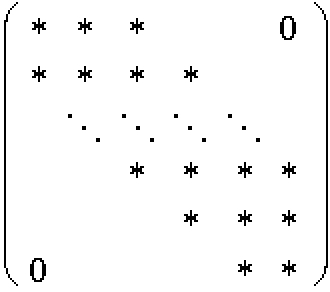
\includegraphics[width=2cm]{images/band.jpg}
  			
  			\item große Matrizen (mit zusätzlichen Eigenschaften)\\
  			$\rightarrow$ \textbf{iterative Methoden:} kenne Startwert
  			$x_0$, berechne neue Approximation $x_i$ unter
  			Ausnutzung der vorherigen bis die
  			\textbf{Näherungslösung} $x_i$ \enquote{gut genug ist}.
  			\end{itemize}
  			
  			\item \textbf{Lineare Ausgleichsprobleme}\\
  			Beispiel:\\
  			Wir messen den Zusammenhang zwischen Spannung U und
  			Stromstärke I\\
  		\parbox[c]{3cm}{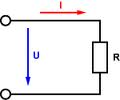
\includegraphics[width=2cm]{images/ohmsche.jpeg} }
  		  \parbox[c]{6cm}{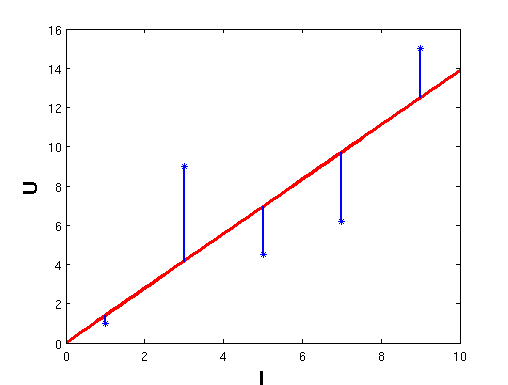
\includegraphics[width=5cm]{images/linausgl2.png}} \\
  				Ohmsches Gesetz: $U = R \cdot I$\\
  				Gesucht ist der Widerstand R. \\
  				($U_i, I_i$) seien die Messdaten mit möglichen Messfehlern.\\
  				Finde nun $R$, sodass 
  				$\; f(R)\, =\,  \min\limits_r \; \sum\limits_i \; (U_i - r \; I_i)^2$
  				
  		\item \textbf{Lösung nichtlinearer Gleichungen},
  		z.B.
  		\begin{itemize}
  			\item Berechnung von Nullstellen $g(x) = 0$
  			\item Berechnung von Fixpunkten $f(x) = x$
  			\end{itemize}  
  			\item \textbf{Eigenwertwertberechnung}
  			 $\quad \boldsymbol A \boldsymbol x =   \lambda \boldsymbol x, \qquad \; \lambda \in \mathbb{C}$
  		
  			
  		\item \textbf{Interpolation}\\
  		Setze Meßdaten zu einer kontinuierlichen Funktion fort, \\
  		aber wie \enquote{glatt}?\\
  		z.B. stückweise konstant, stückweise linear, oder 
  		falls sie
  		eine Schwingung repräsentieren, berechne die zugehörige
  		Fourierreihe  
  		
  		\item \textbf{Berechnung von Integralen} (Quadraturformeln) \\ 
  		Approximation von $\int_a^b \; f(x) \; dx$
  	\end{enumerate}~\\
  	
  	Bei allem spielt die \textbf{Fehleranalyse} eine große Rolle und
  	ihre Grundbegriffe werden in einem extra Abschnitt behandelt.
  	

\chapter{Lineare Gleichungssysteme: Direkte Methoden}
Sei $ A \in \R^{n\times n}$, $b \in \R^n$. Gesucht ist $x\in \R^n$ mit 
\begin{gather*}
	A\cdot x = b
\end{gather*}
Weitere Voraussetzungen sind die Existenz und Eindeutigkeit einer Lösung.
Bemerkung:
\begin{itemize}
	\item Ein verlässlicher Lösungsalgorithmus überprüft dies und behandelt alle Fälle. 
	\item Die Cramersche Regel ist ineffizient (s. Einführung).
	\item Das Inverse für $x=A^{-1}\cdot b$ aufzustellen ist ebenso ineffizient, denn es ist keine Lösung für alle $b\in \R^n$ verlangt und der Algorithmus wird evtl. instabil aufgrund vieler Operationen.
	\item [$\Rightarrow$] Invertieren von Matrizen vermeiden!!
	\item [$\Rightarrow$] Lösen des Linearen Gleichungssystems!!
\end{itemize}

\sectione{Gaußsches Eliminationsverfahren} \label{2.2.1} \index{Gaußsches Eliminationsverfahren}\index{Dreieckszerlegung}
Das Verfahren wurde 1809 von Friedrich Gauß, 1759 von Josepf Louis Lagrange beschrieben und war seit dem 1. Jhd. v. Chr. in China bekannt.

\subsection{Vorwärtselimination} \label{2.1.1}\index{Vorwärtselimination}\index{Vorwärtssubstitution}
Das Gaußverfahren gilt der Lösung eines linearen Gleichungssystems der Form
\begin{align*}
	Ax &= b
\end{align*}
mit $A=(a_{ij})_{i,j \leq n} \in K^{n\times n}$ Matrix und $b=(b_i)_{i\leq n} \in K^n$ Vektor.\\
Der zugehörige Algorithmus sieht folgendermaßen aus:
\begin{gather*}
	\begin{array}{ccccccccc}
	a_{11}x_1 &+& a_{12}x_2 &+& \cdots &+& a_{1n}x_n & = & b_1 ~~\\
	a_{21}x_1 &+& a_{22}x_2 &+& \cdots &+& a_{2n}x_n & = & b_2 \\
	\vdots         &&        \vdots     &&              &&   \vdots       &    & \vdots \\
	a_{n1}x_1 &+& a_{n2}x_2 &+& \cdots &+& a_{nn}x_n & = & b_n \\\\
	&&&& \Downarrow &&&& 
	\end{array} \\
\quad 	(\text{i-te Zeile}) - (\text{1. Zeile})\cdot \frac{a_{i1}}{a_{11}} \Rightarrow a_{i1}=0\\
\begin{array}{ccccccccc}
&&&& \Downarrow &&&&  \\\\
a_{11}x_1 &+& a_{12}x_2 &+& \cdots &+& a_{1n}x_n & = & b_1 \\
				  &+& a_{22}^{(1)}x_2 &+& \cdots &+& a_{2n}^{(1)}x_n & = & b_2^{(1)} \\
				 &&        \vdots     &&              &&   \vdots       &    & \vdots \\
														&& && && a_{nn}^{(1)}x_n & = & b_n^{(1)} \\\\
&&&& \Downarrow &&&&\\
&&&& \vdots &&&&
\end{array} 
\end{gather*}
mit
\begin{align*}
	a_{ij}^{(1)} &= a_{ij}-a_{1j}\cdot \frac{a_{i1}}{a_{11}} & \text{für }i,j = 2, \cdots, n \\
	b_i^{(1)}      &= b_i- b_1\cdot \frac{a_{i1}}{a_{11}}        & \text{für }i = 2, \cdots, n 
\end{align*}
\marginpar{08.10.2014}
In jedem Schritt werden die Einträge der $k$-ten Spalte analog unterhalb der Diagonalen (also $k=1, \cdots, n-1$) eliminiert:
\begin{align*}
	(\text{$i$-te Zeile})- (\text{$k$-te Zeile})\cdot\frac{a_{ik}}{a_{kk}} && \text{für } i=k+1, \cdots ,n 
\end{align*}
Die Reihe 
\begin{gather*}
			A \rightarrow A^{(1)} \rightarrow A^{(2)} \rightarrow \dotsm \rightarrow A^{(n-1)}
\end{gather*}
wird bis zum $n$-ten Schritt fortgeführt, d.h. bis eine obere Dreiecksgestalt eintritt:
\begin{align}
\nonumber
\underbrace{	\begin{pmatrix}
	a_{11} & \dotsm & \dotsm & a_{1n} \\
	             & a_{22}^{(1)} & \dotsm & a_{2n}^{(1)} \\
	             &&              \ddots  &  \vdots \\
	   0        && &                             a_{nn}^{(n-1)}
	\end{pmatrix}}_{\coloneqq R}
	\cdot
	\begin{pmatrix}
		x_1 \\
		x_2 \\
		\vdots \\
		x_n
	\end{pmatrix}
	& =
	\underbrace{\begin{pmatrix}
		b_1 \\
		b_2^{(1)} \\
		\vdots \\
		b_n^{(n-1)}
	\end{pmatrix}}_{\coloneqq z} \\
Rx &= z 	\label{II.1.1} 
\end{align}
wobei für  $i=k+1, \cdots ,n$ die Einträge wie folgt aussehen:
\begin{align}	
	l_{ik} &\coloneqq \frac{a_{ik}^{(k-1)}}{a_{kk}^{(k-1)}} \label{II.1.2} \\
	a_{ij}^{(k)} &= a_{ij}^{(k-1)} - a_{kj}^{(k-1)}\cdot l_{ik} \label{II.1.3}
				 & \text{für } j=k+1, \cdots , n\\ %
	b_i^{(k)} &= b_i^{(k-1)} -b_k^{(k-1)} \cdot   l_{ik}\label{II.1.4}\index{Vorwärtssubstitution}
\end{align}
Dieser Prozess wird \textbf{Vorwärtselimination} genannt.\\

Der zugehörige Algorithmus ist:

\begin{pseudocode}{0.5\linewidth}
	\textbf{for} $ k = 1, \dots , n-1$\\
	|~	\> \textbf{for} $i = k + 1, \dots , n$ \\
	|~	\> |~\> $l_{ik} = a_{ik} /a_{kk}$\\
	|~	\> |~\> \textbf{for} $j = k + 1, \dots , n$ \\
	|~	\> |~\>|~\> $a_{ij} = a_{ij} - l_{ik} a_{kj} $\\
	|~	\> |~\> \textbf{end}\\
	|~	\> |~\> $b_i = b_i -  l_{ik} b_k $\\
	|~	\> \textbf{end} \\
\textbf{end}
\end{pseudocode}

\subsection{Rückwärtselimination}\label{2.1.2}
Für die Lösung des Gleichungssystems ist dann noch die \textbf{Rückwärtssubstitution} \index{Rückwärtssubstitution} nötig:
\begin{align}
	x_n &= \frac{b_n^{(n-1)}}{a_{nn}^{(n-1)}} \label{II.1.5} \\
	x_{n-1} &=  \frac{b_{n-1}^{(n-2)}-a_{n-1,n}^{(n-1)}\cdot x_n}{a_{(n-1)(n-1)}^{(n-2)}} \label{II.1.6} \\
	x_k &= \frac{b_k^{(k-1)}-\sum_{j=k+1}^{n}a_{kj}^{(k-1)}x_j}{a_{kk}^{(k-1)}} \label{II.1.7}
\end{align}

Als Algorithmus:

\begin{pseudocode}{0.5\linewidth}
	\textbf{for} $k = n, n -1, \dots , 1$ \\
	|~		\>$x_k = b_k$ \\
	|~		\>\textbf{for} $j = k + 1, \dots , n$ \\
	|~		\>|~	$x_k = x_k - a_{kj}x_j$ \\
	|~		\>\textbf{end} \\
	|~		\>$x_k = x_k /a_{kk}$ \\
	\textbf{end}
\end{pseudocode}

\subsection{Vorsicht}
	Algorithmen \ref{2.1.1} und \ref{2.1.2} sind nur ausführbar, falls für die sog. \textbf{Pivotelemente $\mathbf{a_{kk}^{(k-1)}}$ } \index{Pivotelement} gilt:
	\begin{gather*}
			a_{kk}^{(k-1)} \neq 0 \quad   \text{für } k=1, \cdots , n
	\end{gather*}
	Dies ist auch für invertierbare Matrizen nicht immer gewährleistet.
	
\subsection{Weitere algorithmische Anmerkungen}	\label{2.1.4}
Matrix $A$ und Vektor $b$ sollten möglichst \textbf{nie} überschrieben werden! (Stattdessen kann eine Kopie überschrieben werden.) \\
Das Aufstellen von $A$ und $b$ ist bei manchen Anwendungen das teuerste, sie gehen sonst verloren. In \ref{2.1.1} wird das obere Dreieck von $A$ überschrieben. Dies ist möglich, da in \eqref{II.1.3} nur die Zeilen $k+1, \cdots, n$ mithilfe der $k$-ten bearbeitet werden. Am Ende steht $R$ im oberen Dreieck von $A$ und $z$ in $b$. \\
Die $l_{ik}$ werden spaltenweise berechnet und können daher anstelle der entsprechenden Nullen (in der Kopie) von $A$ gespeichert werden, d.h.:
\begin{gather}
	\widetilde{L} \coloneqq (l_{ik})  \label{II.1.8}
\end{gather}
und $R$ werden sukzessive in A geschrieben. 
\begin{figure}
	\parbox{\linewidth}{
		\centering
		
\includegraphics[width=2cm]{images/image_missing.jpg}
		}
	\caption{Veranschaulichung der LR-Zerlegung}
	\label{2.1.3.im1}
\end{figure}
Der Vektor $z$ und anschließend der Lösungsvektor $x$ kann in (eine Kopie von) $b$ geschrieben werden.
Wird eine neue rechte Seite $b$ betrachtet, muss \ref{II.1.1} nicht komplett neu ausgeführt werden, da sich $\widetilde{L}$ nicht ändert. Es reicht \ref{II.1.4} zu wiederholen. \\


\subsection{Dreieckszerlegung} \label{2.1.5} \index{Dreieckszerlegung}
Die Dreieckszerlegung einer Matrix $A$ entspricht dem Verfahren aus \ref{2.1.1}, nur ohne die Zeile \eqref{II.1.4}.

\subsection{Vorwärtssubstitution} \index{Vorwärtssubstitution}
Die Vorwärtssubstitution entspricht der in \ref{2.1.4} bzw. dem Verfahren aus \ref{2.1.1} ohne die Bestimmung von $l_{ik}$ und $R$, also nur Schritt \eqref{II.1.4}.

\subsection{Gauß-Elemination zur Lösung von $Ax=b$}\index{Gauß-Eleminator}
\begin{framed}
	\begin{enumerate}[1]
		\item Dreieckszerlegung
		\item Vorwärtssubstitution        $\quad b_i^{(k)} = b_i^{(k-1)} -b_k^{(k-1)} \cdot   l_{ik} $
		\item Rückwärtssubstitution      $\quad x_k = \frac{b_k^{(k-1)}-\sum_{j=k+1}^{n}a_{kj}^{(k-1)}x_j}{a_{kk}^{(k-1)}}$
	\end{enumerate}
\end{framed}

\subsection{Rechenaufwand gezählt in \enquote{flops}} \index{flops}\index{floating point operations}\index{Rechenaufwand}
\textbf{\enquote{flops} }= \textbf{f}loating \textbf{p}oint \textbf{op}eration\textbf{s} \\
\begin{enumerate}
	\item[\textbf{1.}] \textbf{Dreieckszerlegung} 
			\begin{tabbing}
				für $j=k+1, \dots, n\quad$ \= noch ein wenig text danach \kill
				für $j=k+1, \dots, n$ \> 1 Addition, 1 Multiplikation für $a_{ij}$ \\
				für $i=k+1, \dots, n$ \> 1 Division zusätzl. für $ l_{ik}$
			\end{tabbing}
			Dies ist je für $k=1, \dots, n-1$, also ist die Zahl an Additionen und Multiplikationen
			\begin{align*}
				\sum_{k=1}^{n-1}(n-k)^2 &= \sum_{k=1}^{n-1}k^2 \\
				 											&= \frac{(n-1)n(2n-1)}{6} \\
				 									        &= \frac{2n^3-3n^2+n}{6}\, .
			\end{align*}
			Für große $n$ sind das etwa $\frac{n^3}{3}$ Additionen und Multiplikationen und
			\begin{gather*}
				\sum_{k=1}^{n-1} (n-k) = \frac{n^2-n}{2} \approx \frac{n^2}{n}
			\end{gather*}
			Divisionen. \\
			Damit ergibt sich eine Gesamtanzahl an flops von
			\begin{gather*}
				2\cdot\frac{2n^3-3n^2+n}{6} + \frac{n^2-n}{2} 
					= \frac{2}{3} n^3 - \frac{1}{2}n^2 - \frac{1}{6} n
					 \approx \frac{2}{3}n^2
			\end{gather*}
			für große $n$.
			
	\item[\textbf{2.}] \textbf{Vorwärts- bzw. Rückwärtssubstitution}  \\
			Hier ergeben sich je
			\begin{gather*}
				\sum_{k=1}^{n-1} (n-k) = \frac{n^2-n}{2} \approx \frac{n^2}{2}
			\end{gather*}
			Multiplikationen und Additionen sowie 
			$n$ Divisionen für die Rückwärtssubstitution und damit insgesamt \begin{gather*}n^2+n\end{gather*} flops.	
\end{enumerate}
\paragraph{Zusammenfassung}~ \\
Die Dreieckszerlegung benötigt $\mathcal{O}(n^3)$ flops und 
die Vorwärts- bzw. Rückwärtssubstitution $\mathcal{O}(n^2)$ flops.



\subsection{Definition: Landau-Symbole} \index{Landau-Symbole}
Seien $f,g : D\longrightarrow \R, D\subset \R, -\infty\leq a\leq \infty$ und
$(a_n)_{n\in\N}, (b_n)_{n\in\N}$ Folgen in $\R$.
\begin{enumerate}[a)]
	\item $f(x) = \mathcal{O}(g(x))$ für $x\longrightarrow a$, falls
	\begin{gather*}
		\exists U(a), c\in\R:\, \forall x\in U(a) : \quad |f(x)| \leq c\cdot |g(x)|
	\end{gather*}
	(bzw. falls $\lim\limits_{x\rightarrow a}\frac{|f(x)|}{|g(x)|} \leq c$)
	\item $f(x) = o(g(x))$ für $x\longrightarrow a$, falls 
	$\lim\limits_{x\rightarrow a}\frac{|f(x)|}{|g(x)|} = 0$
	\item $a_n = \mathcal{O}(b_n)$ für $n\longrightarrow \infty$, falls
	\begin{gather*}
		\forall \varepsilon > 0 : \, \exists N\in\N : \, \forall n \geq N: \, |a_n| \leq \varepsilon |b_n|
	\end{gather*}
\end{enumerate}

\subsection{Allgemeines zur Aufwandsbetrachtung}\index{Rechenaufwand}
Die Anzahl der Rechenoperationen ist nicht immer ausschalggebend für den Aufwand, da
z.B.
\begin{description}
	\item[Parallelrechner:] In manchen Algorithmen sind Rechenschritte parallel ausführbar.
	Damit entspricht die Zeit nicht der Anzahl an Operationen und es wird zusätzlich
	\enquote{Kommunikationszeit} benötigt.
	\item[Sortieralgorithmen:] Die Indexverwaltung benötigt Zeit, aber keine/kaum Rechenoperationen
	\item[If-When-Abfragen:] entsprechend
\end{description}
Rechenoperationen liefern jedoch oft eine gute Schätzung.

\marginpar{13.10.2014}
\subsection{Formalisieren des Gauß-Algorithmus} \index{Gaußsches Eliminationsverfahren} \index{LR-Zerlegung}


MISSING

\subsection{Lemma (Eigenschaften der $L_k$-Matrizen)} \label{2.1.12} \index{Frobeniusmatrix}
\begin{enumerate}[1.]
	\item $L_k$ ist eine Frobeniusmatrix, d.h. sie unterscheidet sich höchstens
			 in einer Spalte von der Einheitsmatrix $I$.
	\item $L_k^{-1} = I + l_ke_{k}^T$
	\item Es gilt:
			\begin{align}
				L &= L_1^{-1} \cdot \dotsc \cdot L_{n-1}^{-1}  
				\label{II.1.13}
				\\ \nonumber
					& = I + \sum_{i=1}^{n-1} l_i e_i^T \\ \nonumber
					&= \begin{pmatrix}
						1 && 0 ~ \\
						&\ddots& \\
						~l_{ij} && ~1
					\end{pmatrix} \\ \nonumber
					&= I+ \widetilde{L}
			\end{align}
			
			Hiermit folgt: 
\end{enumerate}

\subsection{Satz (LR- oder LU-Zerlegung)} \index{LR-Zerlegung}\index{LU-Zerlegung}
Das obige Verfahren (\eqref{II.1.2} und \eqref{II.1.3}) erzeugt unter der Voraussetzung
von nicht-nullwertigen Pivotelementen eine Faktorisierung
\begin{align*}
	A= L\cdot R 
\end{align*}
wobei $R$ eine obere Dreiecksmatrix und $L$ eine untere, normierte Dreiecksmatrix ist,
d.h. für $i=1, \cdots , n$ gilt $l_{ii}= 1$. \\
Weiterhin existiert zu jeder regulären Matrix höchstens eine solche Zerlegung.

\begin{proof}
MISSING
\index{Verfahren von Crout}
%\begin{figure}
%	\parbox{\linewidth}{
%		\centering
%		
\includegraphics[width=2cm]{images/image_missing.jpg}
%	}
%	\caption{Verfahren von Crout}
%	\label{2.1.13.im1}
%\end{figure}
%\begin{figure}
%	\parbox{\linewidth}{
%		\centering
%		
\includegraphics[width=2cm]{images/image_missing.jpg}
%	}
%	\caption{Verfahren zur LR-Zerlegung}
%	\label{2.1.13.im2}
%\end{figure}
%\begin{figure}
%	\parbox{\linewidth}{
%		\centering
%		
\includegraphics[width=2cm]{images/image_missing.jpg}
%	}
%	\caption{Zeilenweise LR-Zerlegung}
%	\label{2.1.13.im3}
%\end{figure}

\end{proof}

\sectione{Gaußsches Eliminationsverfahren mit Pivotisierung}
\paragraph{Beispiel} Die Matrix $A= \begin{pmatrix}0&1\\1&0\end{pmatrix} $
ist invertierbar, aber die Gauß-Elimination versagt. Permutiere also die erste mit der
zweiten Zeile und der Algorithmus wird anwendbar.

\paragraph{Allgemein} Vermeide die Division durch betragsmäßig kleine Zahlen! 


\subsection{Spaltenpivotisierung (=partielle/ halbmaximale Pivotisierung)} \index{Pivotisierung!Spalten-}\index{Pivotisierung}\index{Pivotisierung!halbmaximale}\index{Pivotisierung!partielle}
Im k-ten  Eliminationsschritt ist\\
\parbox{\linewidth}{
	\centering
	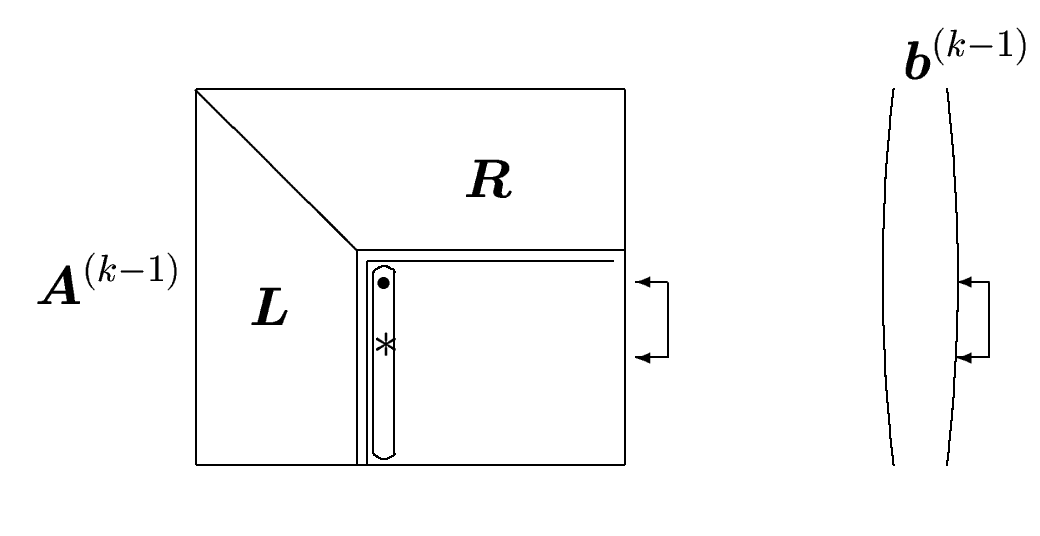
\includegraphics[width=0.5\linewidth]{images/Gausspivot.png}
	\label{2.2.1.im1}
}

MISSING

\subsection{Bemerkung}
\begin{enumerate}[a)]
	\item Hiermit gilt $|l_{jk} \ll 1$.
	\item Anstelle von Spaltenpivotisierung kann eine \textbf{Zeilenpivotisierung}\index{Pivotisierung!Zeilen-}
	durchgeführt werden.
	Welche günstiger (in cpu-time) ist, hängt von der Rechnerarchitektur und
	der damit zusammenhängenden Umsetzung des Gauß-Algorithmus ab.\\
	(Beispielsweise greifen Vektorrechner entweder auf die gesamte Spalte
	oder auf die gesamte Zeile einer Matrix zu und bevorzugen dementsprechend
	Operationen spalten- bzw. zeilenweise.)
	\item Der Aufwand enthält (bis auf $|\cdot |$) keine Rechenoperationen (flops),
	aber $\mathcal{O}(n^2)$ Vergleiche und Vertauschungen.
	\item Eine \textbf{vollständige Pivotsuche}\index{Pivotisierung!vollständige} sucht das betragsmäßig größte Element der gesamten Restmatrix und benötigt $\mathcal{O}(n^3) $ Vergleiche
	(sie wird so gut wie nie angewendet).
\end{enumerate}

Damit die LR-Zerlegung unabhängig von der rechten Seite erstellt werden kann, müssen die Permutationen gespeichert werden.
Hierfür verwendet man  einen sog. \textbf{Permutationsvektor} $\Pi$, wobei
\begin{gather*}
	\Pi^{(k-1)}(r) = s
\end{gather*}
bedeutet, dass nach dem $(k-1)$-ten Eliminationsschritt in der $r$-ten Zeile
von $A^{(k-1)}$ die $s$-te bearbeitete Zeile von $A$ steht, also
\begin{align*}
	\Pi^{(k)}(k) &= \Pi^{(k-1)}(p) \\
	\Pi^{(k)}(p) &= \Pi^{(k-1)}(k)  \quad \text{und entsprechend} \\
	\scriptsize \Pi^{(k)} (i) &= \Pi^{(k)} (i) \quad \text{ für }  i\neq k,p 
\end{align*}
Für die \textbf{Permutationsmatrix}\index{Permutationsmatrix}  
\begin{align*}
	P_{\Pi}&=(e_{\Pi(1)}, \dots , e_{\Pi(n)}) 
	 &&
		 e_j\coloneqq \begin{pmatrix}
		 						 0\\\vdots\\0\\
		 						 1 \\
		 						 0\\\vdots\\0 
		 					  \end{pmatrix}
		 					   \begin{array}{l}
			 					   \\\\
			 					   \shortleftarrow \text{j-te Stelle}\\
			 					   \\\\
		 					   \end{array} \\
\text{mit }	\quad PA&= LR
\end{align*}
gilt
\begin{gather*}
	P^{-1} = P^T
\end{gather*}
und
\begin{gather*}
	\det P_{\Pi} = sign(\Pi) =  \begin{cases}
		+1&  \text{falls }\Pi \text{ von gerader}\\
		-1 &  \text{falls } \Pi \text{ von ungerader}
	\end{cases} \text{ Anzahl an Transpositionen erzeugt wird}
\end{gather*}


\subsection{Gauß-Elimination mit Spaltenpivotisierung}
Der zugehörige Algorithmus zur Spaltenpivotisierung ist: \\

\begin{pseudocode}{0.9\linewidth}
	$\pi(1 : n) = [1 : n] $  \\
	\textbf{for} $k = 1, \dots, n-1$ \\
	~|	  \> bestimme Pivotzeile $p$, so dass\\
	~|	  \>\>	$|a_{pk} | = \max\{|a_{jk} | , j = k, . . . , n\}$ \\
	~|	  \> $\pi(k) \leftrightarrows\footnotemark \pi(p)$ \\
	~|	  \> $A(k, 1 : n) \leftrightarrows A(p, 1 : n)$ \\
	~|	  \> \textbf{if} $a_{kk} \neq 0$ \\
	~|	  	   \>~|\> $zeile = [k + 1 : n]$ \\
	~|	  	   \>~|\> $A(zeile, k) = A(zeile, k)/a_{kk}$ \\
	~|	  	   \>~|\> $A(zeile, zeile) = A(zeile, zeile) - A(zeile, k)A(k, zeile)$\\
	~|	  \> \textbf{else} \\
	~|	  	   \>~|\> \enquote{$A$ ist singulär}\\
	~|	  \> \textbf{end}\\
	\textbf{end}
	\footnotetext{$\leftrightarrows$ bedeutet \enquote{vertausche mit}}
\end{pseudocode}\\

\subsection{Satz: Dreieckszerlegung mit Permutationsmatrix} \label{2.2.4} 
	Für jede invertierbare Matrix $A$ existiert eine Permutationsmatrix $P$,
	so dass eine Dreieckszerlegung
	\begin{gather*}
		PA = LR
	\end{gather*}
	existiert.
	$P$ kann so gewählt werden, dass alle Elemente von $L$ betragsmäßig kleiner oder gleich
	1 sind, d.h.
	\begin{gather*}
		|l_{ij}| \leq 1\quad \forall i, j
	\end{gather*}
	
	
\begin{proof}
	Da $\det A \neq 0$ ist, existiert eine Transposition $\tau_1$, s.d. 
	\begin{gather*}a_{11}^{(1)}= a_{\tau_1, 1} \neq 0 \end{gather*}
	und
	\begin{gather*}
		| a_{\tau_1, 1} | \geq |a_{i1}| 
		\quad \forall i=1, \cdots, n \, . 
	\end{gather*}
	Wir erhalten damit
	\begin{gather*}
		L_1P_{\tau_1} \cdot A = A^{(1)} = \begin{pmatrix}
																	a_{11}^{(1)} && \cdots ~&  ~\\
																	0 \\
																	\vdots && B^{(1)} \\
																	0
																\end{pmatrix}
	\end{gather*}
	und alle Elemente von $L_1 $ sind betragsmäßig kleiner oder gleich 1 sowie
	$\det L_1 = 1 $. \\
	Daraus folgt
	\begin{align*}
		\det B^{(1)} & = \frac{1}{\underbrace{a_{11}^{(1)}}_{\neq 0}} \cdot \det A^{(1)} \\
						 & = \frac{1}{a_{\tau_1, 1}^{(1)}}\cdot \det (L_1) \cdot \det (A) \\
						 & \neq 0 \, .
	\end{align*}
	Also ist $B^{(1)}$ invertierbar. \\
	
	Induktiv erhalten wir dann
	\begin{gather*}
		R = A^{(n-1)} = L_{n-1}P_{\tau_{n-1}} \cdot \dotsc \cdot L_1 P_{\tau_1} \cdot A
	\end{gather*}\\
\marginpar{15.10.2014}
	Da $\tau_i$ nur zwei Zahlen $\geq i $ vertauscht, ist
	\begin{align*}\index{Vorwärtselimination}
		\Pi_i  &\coloneqq \tau_{n-1} \circ \dots \circ \tau_i \quad\text{ für } i=1,\dots (n-1) 
		\end{align*}
	eine Permutation der Zahlen $\{i,\dots, n\}$, d.h. insbesondere gilt:
	\begin{alignat*}{2}
		\Pi_i(j)&=j  & \quad &\text{ für } j=1,\dots,(i-1) \\
		\Pi_i(j)&\in \{i, \dots, n\} & &\text{~für~}j=i,\dots, n\,. 
	\end{alignat*}
	\begin{align*}
		P _{\Pi_{i+1}}  &= (e_1, \dotsc e_i, e_{\Pi_{i+1}(i+1)}, \dotsc, e_{\Pi_{i+1}(n)}) 
								= \begin{pmatrix}
										I_i & 0 \\
										0 & P_{\sigma}
								\end{pmatrix}
	\end{align*}
	Damit folgt:
	\begin{align*}
	P_{\Pi_(i+1)}\cdot L_i\cdot P_{\Pi_{i+1}}^{-1}  &= 
													P_{\Pi_{i+1}} \cdot \left(\begin{array}{ccc|ccc}
																						& I_i & && 0 & \\
																						\cline{1-6}
																						&     & -l_{i+1, i} & & & \\
																						&  0 &  \vdots      & & I_{n-i} &\\
																						&     & -l_{n, i} & &  & 
																					\end{array}\right)
																			\cdot \begin{pmatrix}
																					I_i & 0 \\
																					0 & P_{\sigma}^{-1}
																			\end{pmatrix}\\
	 &= \begin{pmatrix}
				 I_i & 0 \\
				 0 & P_{\sigma}
			 \end{pmatrix} \cdot   \l\cdot  \cdot  \left(\begin{array}{ccc|ccc}
													 & I_i & && 0 & \\
													 \cline{1-6}
												\cdot  	 &     & -l_{i+1, i} & & & \\
													 &  0 &  \vdots      & & P_{\sigma}^{-1} &\\
													 &     & -l_{n, i} & &  & 
												\end{array}\right) \\
	 &= \left(\begin{array}{ccc|ccc}
				 & I_i & && 0 & \\
				 \cline{1-6}
				 &     & -l_{\Pi_{i+1}(i+1), i} & & & \\
				 &  0 &  \vdots      & & I_{n-i} &\\
				 &     & -l_{\Pi_{i+1}(n), i} & &  & 
		 \end{array}\right) \\
	 &= I - (P_{\Pi_{i+1}} l_i)e_i^T\\
	 &\eqqcolon \widehat{L}_i
	\end{align*}
	und
	\begin{align*}		R =&\, L_{n-1}\\
					&\cdot (P_{\tau_{n-1}}L_{n-2}P_{\tau_{n-1}}^{-1})\\
		&				\cdot (P_{\tau_{n-1}}P_{\tau_{n-2}}L_{n-2}P_{\tau_{n-2}}^{-1}P_{\tau_{n-1}}^{-1})\\
		&\; \vdots \\
		&		 \cdot (P_{\tau_{n-1}}\dotsm P_{\tau_{1}}L_{1}P_{\tau_{1}}\dotsm P_{\tau_{n-1}}) \cdot A\\
=&\,L_{n-1}\widehat{L}_{n-2}\dotsm\widehat{L}_1P_{\Pi_{1}}\cdot A
\end{align*}
Nach Lemma \ref{2.1.12} gilt daher, es existiert eine Permutation $\Pi_{1}$ mit
\begin{gather*}
	P_{\Pi_1}\cdot A = LR ,
	\end{gather*}
wobei $R$ obere Dreiecksgestalt hat und
\begin{align*}
		L  &=  \begin{pmatrix}
						1 && & 0\\
						l_{\Pi_2(2),1} & \ddots & \\
						\vdots &            \ddots &  1\\
						l_{\Pi_n(n),1}& \dotsm &  l_{\Pi_n(n),n-1} & 1 
					\end{pmatrix} 
					& \text{mit } |l_{ij}| \leq 1 
\end{align*}
gilt.
\end{proof}

\subsection{Lösen eines Gleichungssystems $Ax=b$} \label{2.2.5}
\subsection{Bemerkungen}
\subsection{Beispiel zur Pivotisierung}


\marginpar{15.10.2014}
\chapter{Fehleranalyse} \index{Fehler}\label{3}
%
\begin{align*}
	\overset{x+\varepsilon \text{ statt } x}{\framebox[3cm]{Eingabe}} \longrightarrow 
	\overset{\underset{\text{\tiny (z.B. durch Rundung)}}{\widetilde{f} \text{ statt } f}}{\framebox[3cm]{Algorithmus}} \longrightarrow
	\overset{\widetilde{f}(x+\varepsilon) \text{ statt } f(x)}{\framebox[3cm]{Resultat\phantom{g}}}
\end{align*}\\

Bei der Fehleranalyse liegt das Hauptaugenmerk auf
\begin{itemize}
	\item[] \textbf{Eingabefehler}\\ z.B.Rundungsfehler, Fehler in Messdaten, Fehler im Modell (falsche Parameter)
	\item[] \textbf{Fehler im Algorithmus} \\ z.B. Rundungsfehler durch Rechenoperationen, Approximationen \\
	 (z.B. Ableitung durch Differenzenquotient oder die Berechnung von Sinus durch abgebrochene Reihenentwicklung)
	\\
	\item[\textit{1. Frage}] Wie wirken sich Eingabefehler auf das Resultat unabhängig vom gewählten Algorithmus aus?
		\item[\textit{2. Frage}]Wie wirken sich (Rundungs-)Fehler des Algorithmus aus?\\
											Und wie verstärkt der Algorithmus Eingabefehler?
\end{itemize}


\sectione{Zahlendarstellung und Rundungsfehler} \label{3.1} \index{Fehler} \index{Rundungsfehler}\index{Zahlendarstellung}
Auf (Digital-)Rechnern können nur endlich viele Zahlen realisiert werden. \\
Die wichtigsten Typen sind: 
\begin{itemize}
	\item \textbf{ganze Zahlen}  (integer)\index{integer}:
					\begin{align*}
						 z&=\pm \sum_{i=0}^{m}z_i\beta_i & \text{mit }
						 \begin{array}{l@{\,}l}
							 \beta &= \text{Basis des Zahlensystems (oft $\beta=2$)} \\
							 z_i &\in \{0, \cdots \beta-1\}
						 \end{array}
						\end{align*}
	\item \textbf{Gleitpunktzahlen} (floating point) \index{floating point}
\end{itemize}

\subsection{Definition: Gleitkommazahl} \label{3.1.1} \index{Gleitkommazahl}
Eine Zahl $x\in\Q$ mit einer Darstellung
\begin{align*}
	x&=\sigma \cdot(a_1 . a_2 \cdots a_t)_{\beta}\cdot \beta^e 
	 = \sigma\beta^e \cdot \sum_{\nu=1}^{t}a_\nu \beta^{-\nu+1}\\\\
&\quad\begin{array}{ll}
	\beta\in\N & \text{Basis des Zahlensystems}\index{Basis}\\
	\sigma \in\{\pm 1\} &\text{Vorzeichen} \\
	m = (a_1 . a_2 \cdots a_t)_{\beta} &\text{Mantisse}\index{Mantisse}\\
	\phantom{m}= \sum_{\nu=1}^{t}a_\nu \beta^{-\nu+1} \\
	a_i \in\{0,\cdots , \beta-1\}&\text{Ziffern der Mantisse}\\
	t\in\N&\text{Mantissenlänge} \\
	e\in\Z &\text{mit }e_{min}\leq e \leq e_{max} \text{ Exponent}
\end{array}
\end{align*}
heißt \textbf{Gleitkommazahl} mit $t$ Stellen und Exponent $e$ zur Basis $b$. \\
Ist $a_1\neq 0$, so heißt $x$ \textbf{normalisierte Gleitkommazahl}\index{normalisierte Gleitkommazahl}

\subsection{Bemerkung} \label{3.1.2}
\begin{enumerate}[a)]
	\item 0 ist keine normalisierte Gleitkommazahl, da $a_1 =  0$ ist.
	\item $a_1\neq 0$ stellt sicher, dass die Gleitkommadarstellung eindeutig ist.
	\item In der Praxis werden auch nicht-normalisierte Darstellungen verwendet.
	\item Heutige Rechner verwenden meist $\beta =2$, aber auch $\beta=8, \beta=16$.
\end{enumerate}

\subsection{Beispiel} \label{3.1.3}
 bit-Darstellung nach IEEE-Standard 754 von floating point numbers \\
 Sei die Basis $\beta=2$.
 
\begin{tabular}{l@{}cccc@{}}
				& Speicherplatz & $t$ & $e_{min}$ & $e_{max}$ \\
				\cmidrule{2-5}
	einfache Genauigkeit (float) \index{floating point} & 32bits = 4Bytes & 24 &-126 & 127 \\
	doppelte  Genauigkeit (double)~~\index{double} & 64bits = 8Bytes& 52 & -1022 & 1023
\end{tabular}\\

Darstellung im Rechner (Bitmuster) für float:
\begin{gather*}
\floatbox{s}{b_0\cdots b_7}{a_2\cdots\cdots a_{24}}\\
\text{(Da $a_1\neq 0$, also $a_1=1$ gilt, wird $a_1$ nicht gespeichert)}
\end{gather*}

Interpretation ($s,b,a_i\in\{0,1\} \forall i$)
\begin{itemize}
		\item$s$ Vorzeichenbit: $\quad \sigma=(-1)^s 
										\Rightarrow \begin{array}{l}
																\sigma(0)=1 \\
																\sigma(1)=-1
															\end{array} $
		\item $b=\sum_{i=0}^{7}b_i\cdot2^i \in \{1, \cdots, 254\}$ speichert den Exponenten mit \\
							$ \quad e = b-\underbrace{127}_\text{Basiswert}$ (kein Vorzeichen nötig) \\
							Beachte: $b_0=\cdots=b_7=1$ sowie $b_0=\cdots=b_7=0$ sind bis auf Ausnahmen keine gültigen Exponenten
		\item $m=(a_1.a_2\cdots a_{24})=1+\sum_{\nu=2}^{24}a_{\nu}2^{1-\nu}$ stellt die Mantisse dar, $a_1=1$ wird nicht abgespeichert.
		\item Besondere Zahlen per Konvention:
		\begin{itemize}
			\item[$x=0$:] $s$ bel., $b=0$, $m=1 \quad \floatbox{s}{0\cdots0}{0\cdots0}$
			\item[$x=\pm\infty$:]  $s$ bel., $b=255$, $m=1  \quad \floatbox{s}{1\cdots1}{0\cdots0}$
			\item[$x=$NaN] $s$ bel., $b=255$, $m\neq 1$
			\item[$x=(-1)^s$] $s$ bel., $b=0$, $m\neq 1$ und x hat die Form $x=(0+\sum_{\nu=2}^{24}a_{\nu}\cdot 2^{1-\nu})\cdot 2^{126}$ (\enquote{denormalized} number)
		\end{itemize}
\end{itemize}

  
% \marginpar{20.10.2014}
\begin{align*}
\intertext{Betragsmäßig \textbf{größte Zahl}:}
	\floatbox{0}{01\cdots 1}{ 1\cdots\cdots 1} && 
	 x_{max} = (2-2^{-23})\cdot 2^{127}  & \approx 3,4 \cdot 10^{38}
\intertext{Betragsmäßig \textbf{kleinste Zahl}:}
	\floatbox{0}{0\cdots 0}{ 0\cdots\cdots 01} && 
	x_{min} = (2-2^{-23})\cdot 2^{-126} = 2^{-149}  & \approx 1,4 \cdot 10^{-45}
\end{align*}

\subsection{Verteilung der Maschinenzahlen} \label{3.1.4}
ungleichmäßig im Dezimalsystem, z. B.
\begin{align*}
		x &= \pm a_1 . a_2 a_3 \cdot 2^e  & -2\leq & e\leq 1 & a_i & \in \{0,1\} 
\end{align*}
\begin{figure}
	\parbox{\linewidth}{
		\centering
		
\includegraphics[width=2cm]{images/image_missing.jpg}
	}
	\caption{Ungleichmäßige Verteilung der Maschinenzahlen im Dezimalsystem}
\end{figure}
ist im Dualsystem gleichmäßig verteilt.

\subsection{Bezeichnungen} \label{3.1.5}
\begin{itemize}
	\item[\textbf{overflow}] es ergibt sich eine Zahl, die betragsmäßig größer ist als die größte maschinendarstellbare Zahl
	\item[\textbf{underflow}] entsprechend, betragsmäßig kleiner als die kleinste positive Zahl
\end{itemize}
Bsp.: overflow beim integer $b=e+127$
\begin{align*}
	\begin{array}{rrr@{}}
	b &= 254                                &11111110 \\
	   &+  \phantom{24}3 &00000011 \\
	   \cline{3-3} %
	 b+3 = 257 \text{ mod } 2^8  &=\phantom{24}1& \xout{1}00000001 
	\end{array}	  
\end{align*}


\subsection{Rundungsfehler} \label{3.1.6}
Habe $x\in \R $ die normalisierte Darstellung
\begin{align*}
	x &= \sigma \cdot \beta^e (\sum_{\nu=1}^{t}a_{\nu}\beta^{1-\nu} + \sum_{\nu=t+1}^{\infty}a_{\nu}\beta^{1-\nu} ) \\
	  &= \sigma \cdot \beta^e (\sum_{\nu=1}^{t}a_{\nu}\beta^{1-\nu} + \beta^{1-t}\sum_{l=1}^{\infty}a_{t+l}\beta^{-l} )
\end{align*}
mit $e_{min} \leq e \leq e_{max}$, dann wird mit $fl(x)$ die gerundete Zahl bezeichnet, wobei $fl(x)$ 
eindeutig gegeben ist durch die Schranke an den \textbf{absoluten Rundungsfehler} \index{Fehler!absoluter Rundungsfehler}
\begin{align*}
	| fl(x) - x | \leq \begin{cases}
								\frac{1}{2}\beta^{e+1+t} & \text{bei symmetrischem Runden}\\
								\beta^{e+1+t}                    & \text{bei Abschneiden}
							\end{cases} \quad .
\end{align*}
Für die \textbf{relative Rechengenauigkeit} \index{Genauigkeit!relative Rechengenauigkeit}folgt somit 
\begin{align*}
\frac{| fl(x) - x | }{|x|} & \leq \begin{cases}
												\frac{1}{2}\beta^{1-t} & \text{bei symmetrischem Runden}\\
												\beta^{1-t}                    & \text{bei Abschneiden}
											\end{cases} \quad .
\end{align*}
Die \textbf{Maschinengenauigkeit} \index{Genauigkeit!Maschinengenauigkeit} des Rechners ist daher durch 
\begin{align*}
	  eps &= \beta^{1-t} & \text{(für float}\approx 10^{-7}  \text{, für double} \approx10^{-16} )
\end{align*}
gegeben.

Die Mantissenlänge bestimmt also die Maschinengenauigkeit. Bei einfacher Genauigkeit ist $fl(x)$ bis auf ungefähr 7 signifikante Stellen genau. \\
Im Folgenden betrachten wir symmetrisches Runden und definieren daher
\[ \tau \coloneqq \frac{1}{2}eps\]
Weiterhin gilt:
\begin{enumerate}[a)]
	\item Die kleinste Zahl am Rechner, welche größer als 1 ist, ist
					\[ 1 + eps \]
	\item Eine Maschinenzahl x repräsentiert eine Eingabemenge
					\[  E(x) = \{\widetilde{x} \in \R : |\widetilde{x}-x| \leq \tau|x|\} \] \\
				\begin{figure}
					\parbox{\linewidth}{
						\centering
						
\includegraphics[width=2cm]{images/image_missing.jpg}
					}
					\caption{Eingabemenge einer Maschinenzahl}
				\end{figure}
\end{enumerate}

\subsection{Bemerkung} \label{3.1.7}
Gesetze der arithmetischen Operationen gelten i.A. nicht, z.B.
\begin{itemize}
	\item 	$x$ Maschinenzahl $\quad \Rightarrow fl(x+\nu) = x \text{     für }|\nu| < \tau |x|$
	\item Assoziativ- und Distributivgesetze gelten nicht, z.B. für $\beta = 10, \, t=3, \, a=0,1 ,\, b= 105 , \, c= -104$ gilt:
					\begin{align*}
						fl(a+fl(b+c)) &= 1,1 \\
						fl(fl(a+b)+c) &= fl(fl(105,1) + (-104) ) \\
							                &= fl(105-104) \\
							                &= 1 \quad \lightning
					\end{align*}
	\item[ $\Rightarrow$] Für einen Algorithmus ist die Reihenfolge der Operationen wesentlich!
									  Mathematisch äquivalente Formulierungen können zu verschiedenen Ergebnissen führen.
\end{itemize}

\subsection{Auslöschung von signifikanten Stellen} \label{3.1.8}
Sei $x=9,995\cdot 10^{-1}, y=9,984 \cdot 10^{-1}$. Runde auf drei signifikante Stellen und berechne $x-y$:
\begin{align*}
	\widetilde{f}(x,y) &\coloneqq fl(fl(x)- fl(y)) = fl(1,00\cdot 10^0 - 9,98\cdot 10^{-1}) \\
							  &= 	fl(0,02\cdot 10^{-1}) \\
							  &= fl(2,00 \cdot 10^{-3}) \\
	f(x,y)  &\coloneqq x-y \\
		      &\coloneqq 0,0011 = 1,1\cdot 10^{-3}
	\intertext{Daraus ergibt sich der relative Fehler}
	\frac{|\widetilde{f}(x,y)-f(x,y)|}{|f(x,y)|}
		     &= \frac{|2\cdot 10^{-3}- 1,1\cdot 10^{-3}|}{|1,1\cdot 10^{-3}}
		       = 82\%
\end{align*}
Der Grund hierfür ist, dass das Problem der Substraktion zweier annähernd gleich großer Zahlen
schlecht konditioniert ist.\\

\textbf{Zwei Regeln:}
\begin{enumerate}[1)]
	\item Umgehbare Substraktion annähernd gleich großer Zahlen vermeiden!
	\item Unumgängliche Substraktion möglichst an den Anfang des Algorithmus stellen! (siehe später)
\end{enumerate}

% 2.2
%-----------------------------------------------------------------------------------------------------------------------------------------
\sectione{Kondition eines Problems} \label{3.2}
Es wird das Verhältnis 
\begin{gather*}
	\frac{\text{Ausgabefehler}}{\text{Eingabefehler}}
\end{gather*}
untersucht.

\subsection{Definition: Problem} \label{3.2.1} \index{Problem}
Sei $f: U \subseteq \R^n \rightarrow \R^m$ mit $U$ offen und sei $x\in U$. Dann bezeichne $(f, x)$ das Problem, zu einem gegebenen $x$ die Lösung $f(x)$ zu finden.

\subsection{Definition: absoluter und relativer Fehler} \label{3.2.2} \index{Fehler}
Sei $x\in\R^n$ und $\widetilde{x} \in \R^n$ eine Näherung an $x$. Weiterhin sei $\|\cdot\|$ eine Norm auf $\R^n$.
\begin{itemize}
	\item[a)] $\nn{\widetilde{x} - x}$ heißt \textbf{absoluter Fehler} \index{Fehler!absoluter}
	\item[b)] $\frac{\nn{\widetilde{x} - x}}{\nn{x}}$ heißt \textbf{relativer Fehler}\index{Fehler!relativer}
\end{itemize}
Da der relative Fehler skalierungsinvariant ist, d.h. unabhänging von der  Wahl von $x$ ist, ist dieser i.d.R. von größerem Interesse.
Beide Fehler hängen von der Wahl der Norm ab!
Häufig werden Fehler auch komponentenweise gemessen:
\begin{align*}
	\text{Für } i=1,\cdots , n : && |\widetilde{x}_i - x_i | & \leq \delta & \text{ (absolut)} \\
											 && |\widetilde{x}_i - x_i | &\leq \delta |x_i| & \text{ (relativ)}
\end{align*}

\subsection{Wiederholung: Normen} \label{3.2.3}\index{Norm}

\begin{align*}
	\text{Euklidische Norm ($l_2$-Norm):} &&	\nn{x}_2 &\coloneqq \sqrt{\sum_{i=1}^{n}|x_i|^2}
		\index{Norm!Euklidische Norm} \\
			IMAGE~MISSING \\
	\text{Maximumsnorm ($l_\infty$-Norm):} &&\nn{x}_\infty &\coloneqq \max\{|x_i| : i=1, \cdots n\} \\
	  	\index{Norm!Maximumsnorm}
		  	IMAGE~MISSING \\
	\text{Summennorm ($l_1$-Norm):} &&	\nn{x}_1 &\coloneqq \sum_{i=1}^{n}|x_i| 
		\index{Norm!Summennorm}\\
			IMAGE~MISSING \\
	\text{Hölder-Norm ($l_p$-Norm):} &&	\nn{x}_p &\coloneqq 
		\left(\sum_{i=1}^{n}|x_i|^p\right)^{\frac{1}{p}} 
		\index{Norm!Hölder-Norm}
\end{align*}

\subsection{Definition: Matrixnorm} \label{3.2.4}
Auf dem $\R^n$  sei die Norm $\nn{\,\cdot\,}_a$ und auf dem $\R^m$ die Norm $\nn{\,\cdot\,}_b$ gegeben.
Dann ist die zugehörige \textbf{Matrixnorm} \index{Norm!Matrixnorm} gegeben durch:
\begin{align}
	\nn{A}_{a,b} &\coloneqq \sup_{x\neq 0} \frac{\nn{Ax}_b}{\nn{x}_a} \\ \nonumber
					 &= \sup_{\nn{x}_a=1} \nn{Ax}_b \label{III.2.1} 
\end{align}
Also ist   $\nn{A}_{a,b}$ die kleinste Zahl $c>0$ mit
\begin{gather*}
	\nn{Ax}_b  \leq c\nn{x}_a \quad\quad \forall x\in \R^n
\end{gather*}

\subsection{Definition: Frobeniusnorm, p-Norm, Verträglichkeit} \label{3.2.5}
Sei $A\in \R^{m\times n}$.
\begin{enumerate}[a)]
	\item \textbf{Frobeniusnorm} (Schurnorm):
			 $ \quad \nn{A}_F \coloneqq \sqrt{\sum_{i=1}^{m}\sum_{j=1}^{n}|a_{ij}^2|}
				 \index{Norm!Frobeniusnorm}$
    \item \textbf{p-Norm}: 
			 $\quad \nn{A}_p \coloneqq \nn{A}_{p,p}
				 \index{p-Norm}$
    \item Eine Matrixnorm heißt \textbf{verträglich} \index{Norm!verträglich} mit den Vektornormen 
			    $\nn{\,\cdot\,}_a, \nn{\,\cdot\,}_b$, falls gilt
			    \footnote{ Beachte: $\nn{A}_{a,b}$ ist die kleinste Norm im Gegensatz zu $\nn{A}$, welche hier beliebig ist.}:
				 \begin{gather*}
					 	\nn{Ax}_b \leq \nn{A}\cdot \nn{x}_a \quad \forall x\in \R^n
				 \end{gather*}
\end{enumerate}

\subsection{Bemerkungen} \label{3.2.6}
\begin{enumerate}[a)]
	\item Die Normen $\nn{\,\cdot\,}_F$ und $\nn{\,\cdot\,}_p$ sind \textbf{submultiplikativ} \index{Norm!submultiplikative}, d.h.
				\begin{gather*}
					\nn{A\cdot B} \leq \nn{A}\cdot\nn{B}
				\end{gather*}
	\item Die Norm $\nn{\,\cdot\,}_{1,1}$ wird auch \textbf{Spaltensummennorm}\index{Norm!Spaltensummennorm} genannt:
				\begin{gather*}
					\nn{A}_1 = \max_{1\leq j \leq n}\sum_{i=1}^{m}|a_{ij}|
				\end{gather*}
			Sie ist das Maximum der Spaltensummen\footnote{Beweis: siehe Übungsblatt 3}.
	\item Die Norm $\nn{\,\cdot\,}_{\infty, \infty}$ wird auch \textbf{Zeilensummennorm} \index{Zeilensummennorm}
	 genannt\footnote{Beweis: siehe Übungsblatt 3}:
	%not sure, why \footref won't work here ...
				\begin{gather*}
					\nn{A}_\infty = \max_{1\leq i \leq m}\sum_{j=1}^{n}|a_{ij}|
				\end{gather*}
	\item Die Frobeniusnorm $\nn{\,\cdot\,}_F$ ist verträglich mit der euklidischen Norm $\nn{\,\cdot\,}_2$
	\item Die Wurzeln aus den Eigenwerten von $A^TA$ heißen \textbf{Singulärwerte $\sigma_i$} \index{Singulärwert} von A.
	Mit ihnen kann die $\nn{\,\cdot\,}_{2,2}$ Norm dargestellt werden\footnote{Beweis: siehe Übungsblatt 3}:
				\begin{align*}
					\nn{A}_2 &= max \{\sqrt{\mu} : A^TA\cdot x = \mu x\text{ für ein }x\neq 0 \} \\
								& = \sigma_{max}
				\end{align*}
\end{enumerate}


\marginpar{22.10.2014}
%ultimate evil hack to go along with numeration
%\minisec{\Large3.2 a) Normweise Konditionsanalyse} \label{3.2a}\vspace{1eM}
\extrasection{a)}{Normweise Konditionsanalyse}
%%Alternative to add it to table of contents:
%\renewcommand{\thesubsection}{\thesection.a)}
%\setkomafont{subsection}{\Large}
%\subsection{NORMWEISE KONDITIONSANALYSE}
%\renewcommand{\thesubsection}{\thesection.\arabic{subsection}}
%\addtocounter{subsection}{-1}
%\setkomafont{subsection}{\large}

\subsection{Definition: absolute und relative normweise Kondition}\index{normweise Kondition}
Sei $(f,x)$ ein Problem mit $f:U\subset \R^n \rightarrow \R^m$
und $\nn{\,\cdot\,}_a$ auf $\R^n$ und $\nn{\,\cdot\,}_b$ auf $\R^m$ eine Norm.
\begin{enumerate}[a)]
	\item Die \textbf{absolute normweise Kondition}\index{Kondition!normweise, absolut} eines Problems $(f,x)$ ist die kleinste Zahl 
			 $\kappa _{abs} > 0 $ mit
			 \begin{align}
			 	\nn{f(\widetilde{x})-f(x)}_b &\leq \kappa _{abs}(f,x) \nn{\widetilde{x}-x}_a
			 	+ o\left(\nn{\widetilde{x}-x}_a\right) \label{III.2.2} \\\nonumber
			 	\Bigl(f(\widetilde{x})- f(x) 
						 	&=\underbrace{ f'(x)(\widetilde{x}-x)\pm o\left(\nn{\widetilde{x}-x}\right)}_{Taylorentwicklung}
							 \quad \text{für }\widetilde{x}\rightarrow x 
						 	\Bigr)
			 \end{align}
	\item Die \textbf{relative normweise Kondition}\index{Kondition!normweise. relativ} eines Problems $(f,x)$  mit $x\neq 0, f(x) \neq 0$
			 	ist die kleinste Zahl 
			 	$\kappa _{rel} > 0 $ mit
			 	\begin{align}
			 \frac{	\nn{f(\widetilde{x})-f(x)}_b }{\nn{f(x)}_b}
				 &\leq \kappa _{rel}(f,x)\frac{ \nn{\widetilde{x}-x}_a}{\nn{x}_a}
			 	+ 
			 	o\left(\frac{\nn{\widetilde{x}-x}_a}{\nn{x}_a}\right) \label{III.2.3}
					 &&	\text{für } \widetilde{x} \rightarrow x
			 	\end{align}
	\item Sprechweise:
		\begin{itemize}\index{Kondition!gut/schlecht konditioniert}
			\item falls $\kappa$ \enquote{klein} ist, ist das Problem \enquote{gut konditioniert}
			\item falls $\kappa$ \enquote{groß} ist, ist das Problem \enquote{schlecht konditioniert}
		\end{itemize}
\end{enumerate}

\subsection{Lemma} \label{3.2.8}
Falls $f$ differenzierbar ist, gilt
\begin{gather}
	\kappa_{abs}(f,x) = \nn{Df(x)}_{a,b} \label{III.2.4}
\end{gather}
und für $f(x) \neq 0$
\begin{gather}
	\kappa_{rel}(f,x) = \frac{\nn{x}_a}{\nn{f(x)}_b}\cdot \|Df(x)\|_{a,b} \label{III.2.5}
\end{gather}
wobei $Df(x)$ die Jakobi-Matrix bezeichnet.
%
\subsection{Beispiel: Kondition der Addition}\label{3.2.9} \index{Kondition!Addition}
$f(x_1, x_2) \coloneqq x_1 +x_2 , \, f:\R^2 \rightarrow \R$. \\
Wähle $l_1$-Norm auf $\R^2$ (und $\R$)
\begin{align*}
			Df(x_1, x_2) \, =(\nabla f^T) \, &= (\frac{\partial}{\partial x_1}f, \frac{\partial}{\partial x_2}f )\\
				&= (1,1) && \text{(Matrix!)}
\end{align*}
damit
\begin{align*}
	\kappa_{abs} (f,x)&= \nn{Df(x)}_{1,1} && \text{(Matrix-Norm!!)}\\
						 		&= \nn{Df(x)}_1 \\
								&=1 \\
	\kappa_{rel} (f,x) &= \frac{\nn{x}_1}{\nn{f(x)}_1} \cdot \nn{Df(x)}_{1} \\
								&= \frac{|x_1| + |x_2|}{|x_1+x_2|}
\end{align*}
Daraus folgt: Die Addition zweier Zahlen mit gleichem Vorzeichen ergibt
\begin{gather*}
	\kappa_{rel} = 1
\end{gather*}
Die Subtraktion zweier annähernd gleich großer  Zahlen ergibt eine sehr schlechte relative
Konditionierung:
\begin{gather*}
\kappa_{rel} \gg 1
\end{gather*}
Zum Beispiel in \ref{3.1.8}: Es ist 
\begin{align*}
	x &= \begin{pmatrix}
		9,995 \\
		-9,984
	\end{pmatrix}
	\cdot 10^{-1} \\
	\widetilde{x} = fl(x) &= \begin{pmatrix}
		1 \\
		-9,98\cdot 10^{-1}
	\end{pmatrix}
\intertext{also}
	\frac{|f(\widetilde{x})-f(x)|}{|f(x)|}	&= \frac{0,9}{1,1} 
															= 0,\overline{81} \\
															&\leq \kappa_{rel}(f,x)\cdot \frac{\|\widetilde{x}-x\|_1}{\|x\|_1} \\
															&= \kappa_{rel}(f,x) \cdot 4,6\cdot 10^{-4}
\end{align*}
%

\subsection{Beispiel: Lösen eines Gleichungssystems} \label{3.2.10}
Sei $A\in \R^{n\times n}$ invertierbar und $b\in \R^n$. Es soll 
\begin{gather*}
	Ax =b
\end{gather*}
gelöst werden.
Die möglichen Lösungen in $A$ und in $b$ lassen sich folgendermaßen ermitteln:
\begin{enumerate}[a)]
	\item Betrachte die Störungen in $b$:\\
			Sei hierzu
			\begin{gather*}
			f: b\mapsto x= A^{-1}b 
			\end{gather*}
			Berechne dann $ \kappa(f,b)$ und löse 
			\begin{align*}
					A(x + \Delta x) &= b+\Delta b \\
					f(b + \Delta b) - f(b) &= \Delta x \\
													&= A^{-1} \cdot \Delta b && \text{da }x = A^{-1}b \\
					\Rightarrow \|\Delta x\|_{b}  &= \|A^{-1}\Delta b\|_{b} \\
														&\leq \|A^{-1}\|_{a,b}\cdot \|\Delta b\|_{b} && \forall b, \Delta b 
			\end{align*}
			wobei $\|\cdot\| $ auf $\Renn$ die dem $\Ren$ zugeordnete Matrix-Norm sei. \\
			Die Abschätzung ist \textbf{scharf}\index{scharf}, d.h. es gibt ein $\Delta b\in \R^n$, so dass \enquote{=} gilt, nach Definition \ref{3.2.4}. \\
			Also gilt\footnote{vgl. auch Lemma \ref{3.2.8}: $\kappa_{abs}(f,b)=\nn{Df(b)}_{a,b}=\nn{A^{-1}}_{a,b}$}:
			\begin{gather}
				\kappa_{abs}(f,b) = \nn{A^{-1}}_{a,b} \label{III.2.6}
			\end{gather}
			unabhängig von b.  $ \quad \left( x\mapsto Ax \quad \kappa_{abs}\right)$\\
			Ebenso folgt die scharfe Abschätzung 
			\begin{align}
				\nonumber
				\frac{\|	f(b + \Delta b) - f(b)\|}{\|f(b)\|} &= \frac{\nn{\Delta x}}{\nn{x}}\\ \nonumber
						& = \frac{\nn{A^{-1}\Delta b}}{\nn{x}} \\ \nonumber
						& \leq  \frac{\|A^{-1}\|\cdot \|b\|}{\|x\|} \cdot \frac{\|\Delta b\|}{\|b\|} \\
				\intertext{Damit}
				\kappa_{rel} (f,b) &= \|A^{-1} \| \cdot \frac{\|b\|}{\|A^{-1}\cdot b\|} \label{III.2.7}
			\end{align}
			Da $\|b\| \leq \|A\|\cdot\|x\| = \|A\|\cdot \|A^{-1}b\|$ folgt:
			\begin{gather}
				\kappa_{rel}(f,b) \leq \|A\| \cdot \|A^{-1}\| \label{III.2.8}
			\end{gather}
			für alle (möglichen rechten Seiten) $b $.\\
			\ref{3.2.8} ist scharf in dem Sinne, dass es ein $\widehat{b}\in \R^n$ gibt 
			mit 
			\begin{gather*}
				\|\widehat{b}\| = \nn{A}\cdot \nn{\widehat{x}}
			\end{gather*}
			und somit
			\begin{gather*}
				\kappa_{rel}(f,\widehat{b}) = \nn{A}\cdot \| A^{-1}\|
			\end{gather*} %
			%
	\item Betrachte die Störungen in $A$:\\
			Löse also 
			\begin{gather*}
				(A+\Delta A)(x+\Delta x) = b
			\end{gather*}
			Sei hierzu
			\begin{align*}
				f:A&\mapsto x= A^{-1}b \\
				\R^{n\times n}&\rightarrow \R^n
			\end{align*}
			und berechne $\kappa(f,A)$ mittels Ableitung $Df(A):\R^{n\times n} \rightarrow \R^n$:
			\begin{align*}
				C\mapsto Df(A) C&= \frac{d}{dt} \left((A+tC)^{-1} \cdot b\right) \Big\vert_{t=0} \\
										  & = \frac{d}{dt}\left((A+tC)^{-1}\right)\Big\vert_{t=0}\cdot b
			\end{align*}			
			Weiterhin gilt
			\begin{align}
				\frac{d}{dt} \left((A+tC)^{-1}\right) \Big\vert_{t=0} &= -A^{-1}CA^{-1}, \label{III.2.9}
			\end{align}
			da
			\begin{align*}
				0&= \frac{d}{dt}I \\
				  &= \frac{d}{dt}\left( (A+tC)(A+tC)^{-1}\right)\\
				  &= C(A+tC)^{-1} +(A+tC)\cdot \frac{d}{dt}(A+tC)^{-1} \\
				  \Leftrightarrow \frac{d}{dt} (A+ tC)^{-1} 
				  &= -(A+tC)^{-1} \cdot C(A+tC)^{-1} \, ,
			\end{align*}
			falls $(A+tC)$ invertierbar ist. Für ein genügend kleines $t$ ist das gewährleistet, da $A$ invertierbar ist (s. Lemma \ref{3.2.12}).
			\begin{gather*}
				\Rightarrow Df(A) C = -A^{-1}CA^{-1}b
			\end{gather*}
			Somit folgt
			\begin{align}
				\nonumber
				\kappa_{abs} (f,A) &= \|Df(A)\| \\ \nonumber
											  &= \sup_{\substack{
																C\neq 0 \\ 
																C\in \R^{n\times n}											  	
														  	}}
														  \frac{\|A^{-1}CA^{-1}b\|}{\|C\|} \\ \nonumber
											  &\leq \sup_{\substack{
															 	C\neq 0 \\ 
															 	C \in \R^{n\times n}														  	
															 }}
												 \frac{\|A^{-1}\|\cdot\|C\|\cdot\|A^{-1}b\|}{\|C\|} \\ \nonumber
											  &= \|A^{-1}\| \cdot\|x\| \\ \nonumber
											  &\leq   \|A^{-1}\|^2 \cdot\|b\| \\ \nonumber
				 \kappa_{rel}(f,A)  &= \frac{\|A\|}{\|f(A)\|} \cdot \|Df(A)\| \\
											 &\leq \|A\|\cdot \|A^{-1}\| \label{III.2.10}
			\end{align}
	 \item betrachte Störungen in $A$ und $b$ :
		 \begin{gather*}
		 	(A+\Delta A)(x+\Delta x) = (b+\Delta b) 
		 \end{gather*}
		 Für $\kappa$ müsste $\|(A,b)\|$ festgelegt werden. Dies wird jedoch nicht betrachtet. Es gilt aber folgende Abschätzung für invertierbare Matrizen $A\in \Renn $ und Störungen
		 $\Delta A \in \R^{n\times n}$ mit $\|A^{-1}\|\cdot \|\Delta A\| < 1$:
		 \begin{align}
			 \frac{\|\Delta x\|}{\|x\|} & \leq \|A\| \cdot \|A^{-1}\|\cdot (1- \|A^{-1}\|\cdot \|\Delta A\|) 
													 \cdot
													 \underbrace{\left(  \frac{\|\Delta b\|}{\|b\|} +  \frac{\|\Delta A\|}{\|A\|}  \right)}_{\neq  \frac{\|(\Delta A, \Delta b)\|}{\|(A,b)\|} }
													 \label{III.2.11}
		 \end{align}
		 \begin{proof} s. Übungsblatt \end{proof}
\end{enumerate}

\subsection{Definition: Kondition einer Matrix} \index{Kondition!Matrix}
Sei $\|\cdot\|$ eine Norm auf $\R^{n\times n} $ und $A\in \R^{n\times n}$ eine reguläre Matrix.
Die Größe
\begin{gather*}
	\kappa_{\|\cdot\|}(A) = cond_{\|\cdot\|} \coloneqq \|A\| \cdot \|A^{-1}\|
\end{gather*}
heißt \textbf{Kondition der Matrix} bzgl. der Norm ${\|\cdot\|}$. \\
Ist  ${\|\cdot\|}$ von einer Vektor-Norm ${\|\cdot\|}_p$ induziert, bezeichnet 
	$cond_p(A)$
die $cond_{\|\cdot\|_p}(A)$. Wir schreiben $cond(A)$ für $cond_2(A)$. \\
$cond_{\|\cdot\|}(A) $ schätzt die relative Kondition eines linearen GLS $Ax=b$ für alle möglichen 
Störungen in $b$ oder in $A$ ab und diese Abschätzung ist scharf. \\

Es stellt sich nun die Frage: \\
\textit{Wann existiert die Inverse der gestörten invertierbaren Matrix $A$?} \\
Hierzu werden wir die Relationen benötigen:
\begin{align*}
	A+\Delta A &= A (I+A^{-1}\Delta A)\\
\intertext{und mit $C \in \Renn,\, \|C\| < 1$}
	(I-C)^{-1} &= \sum_{k=0}^{\infty}C^k \\
	\|	(I-C)^{-1} \| &\leq \frac{1}{1-\|C\|}
\end{align*}

\marginpar{27.10.2014}
\subsection{Lemma (Neumannsche Reihe)}\index{Neumannsche Reihe}\label{3.2.12}
\addtocounter{equation}{1}
Sei $C\in\Renn$ mit $\|C\|<1$ und mit einer submultiplikativen Norm $\|\cdot\|$,
so ist $(I-C)$ invertierbar und es gilt:
\begin{gather*}
	(I-C)^{-1}=\sum_{k=0}^{\infty}C^k
\end{gather*}
Weiterhin gilt:
\begin{gather*}
	\|(I-C)^ {-1}\| \leq \frac{1}{1-\|C\|}
\end{gather*}

\begin{proof}
Es gilt zu zeigen, dass $\sum_{k=1}^{\infty}C^k$ existiert: \\
Sei $q\coloneqq \|C\| < 1$, dann gilt: 
\begin{align*}
	\nn{ \sum_{k=0}^{m} C^k } &\leq \sum_{k=0}^{m} \nn{C^k }  && \text{Dreiecksungleichung} \\
								 &\leq \sum_{k=0}^{m}\nn{C}^k && \text{da $\nn{\,\cdot\,}$ submultiplikativ}\\
								 &=\sum_{k=0}^{m}q^k  \\
								 &= \frac{1-q^{m+1}}{1-q} \\
								 &\leq \frac{1}{1-\nn{C}} && \forall m\in \N, \text{ da } q<1 \text{ (geometr. Reihe)}
\end{align*}
Daraus folgt bereits, dass $\sum_{k=1}^{\infty}C^k$ existiert (nach Majorantenkriterium).\\
Weiter gilt dann:
\begin{align*}
	(I-C) \sum_{k=1}^{\infty}C^k &= \lim\limits_{m\rightarrow \infty}(I-C)   \sum_{k=1}^{m}C^k \\
													&= \lim\limits_{m\rightarrow \infty} (C^0-C^{m+1}) \\
													&=I 
\end{align*}
\end{proof}

\subsection{Bemerkung}\label{3.2.13}
\begin{enumerate}[a)]
	\item Für symmetrische, positiv definite Matrix $A\in \Renn$ gilt\footnote{Beweis: siehe Übungsblatt 3}: 
	\begin{gather}
		\kappa_2(A) = \frac{\lambda_{max}}{\lambda_{min}} \label{III.2.13}
	\end{gather}
	\item Eine andere Darstellung von $\kappa(A)$ ist
	\begin{gather}
		\kappa(A) \coloneqq 
		\frac{\underset{\|x\|=1}{\max}\|Ax\|}{\underset{\|x\|=1}{\min}\|Ax\|} \in  \left[ 0, \infty \right]
			 \label{III.2.14}
	\end{gather}
	Diese ist auch für nicht invertierbare und rechteckige Matrizen wohldefiniert. \\
	Dann gilt offensichtlich:
	\item $\kappa(A) \geq 1$
	\item $\kappa(\alpha A)=\kappa(A) \quad \text{für } 0\neq\alpha\in\R$ (skalierungsinvariant)
	\item $A\neq 0$ und $A\in\Renn $ ist genau dann singulär, wenn $\kappa(A)=\infty$. \\
			Wegen der Skalierungsinvarianz ist die Kondition zur Überprüfung der Regularität von $A$ 
			besser geeignet als die Determinante.
	\end{enumerate}
	

\subsection{Beispiel: Kondition eines nichtlinearen Gleichungssystems}
Sei $f:\Ren\rightarrow\Ren$ stetig differenzierbar und $y\in\Ren$ gegeben. \\
Löse
\begin{gather*}
	f(x) = y
\end{gather*}
Gesucht:
\begin{gather*}
	\kappa(f^{-1},y)
\end{gather*}
mit $f^{-1}$ Ausgabe und $y$ Eingabe. \\
Sei $Df(x)$ invertierbar, dann existiert aufgrund des Satzes für implizite Funktionen die inverse Funktion $f^{-1}$ lokal in einer Umgebung von $y$ mit $f^{-1}(y)=x$, sowie
\begin{gather*}
	D(f^{-1})(y) = (Df(x))^{-1}
\end{gather*}
Hiermit folgt:
\begin{align}
	\nonumber
	\kappa_{abs}(f^{-1},y) &= \|(Df(x))^{-1}\| \\
	\kappa_{rel}(f^{-1},y) &= \frac{\|f(x)\|}{\|x\|}\cdot\|(Df(x))^{-1}\|  \label{III.2.15}
\end{align}
Für skalare Funktionen $f:\R\rightarrow\R$ folgt somit:
\begin{gather*}
	\kappa_{rel}(f^{-1},y) = \frac{|f(x)|}{|x|}\cdot \frac{1}{|f'(x)|}
\end{gather*}
Falls $|f'(x)|\rightarrow 0$ ist es eine schlechte absolute Kondition. \\
Für $|f'(x)| \gg 0$ ist es eine gute absolute Kondition.\\
\begin{figure}
	\parbox{\linewidth}{
		\centering
		
\includegraphics[width=2cm]{images/image_missing.jpg}
	}
	\caption{Gute und schlechte Kondition}
\end{figure}

Damit bedeutet eine kleine Störung in $y$ eine große Störung in $x$.


%\minisec{\Large3.2 b) Komponentenweise Konditionsanalyse} \label{3.2b}\vspace{1eM}
\extrasection{b)}{Komponentenweise Konditionsanalyse}

\subsection{Beispiel}
Falls $A$ Diagonalgestalt hat, sind die Gleichungen unabhängig voneinander (entkoppelt)\index{entkoppelt}.
Die erwartete relative Kondition wäre dann -- wie bei skalaren Gleicungen -- stets gleich 1.
Ebenso sind Störungen nur in der Diagonale zu erwarten. Jedoch:
\begin{align*}
	A  &=\begin{pmatrix}
					1 & 0\\
					0 & \varepsilon
				\end{pmatrix} \\
	\Rightarrow 	A^{-1}&=\begin{pmatrix}
													1 & 0\\
													0 & \varepsilon^{-1}
												\end{pmatrix}\\
	\Rightarrow \kappa_\infty& = \kappa_2 = \frac{1}{\varepsilon} 
													&& \text{für }0 < \varepsilon \leq 1											
\end{align*}

\subsection{Definition: Komponentenweise Kondition}\index{Kondition!komponentenweise}
Sei $(f, x) $ ein Problem mit $f(x)\neq 0$ und $x=(x_i)_{i=1,\cdots , n}$ mit $x_i\neq 0 $  für alle $i=1,\cdots, n$.
Die \textbf{komponentenweise Kondition} von $(f,x) $ ist die kleinste Zahl $\kappa_{rel}\geq 0$, so dass:
\begin{align*}
	\frac{\|f(\widetilde{x})-f(x)\|_\infty}{\|f(x)\|_\infty} 
				&\leq \kappa_{rel} \cdot \underset{i}{\max}\frac{|\widetilde{x_i}-x_i|}{|x_i|}+ o\left(\underset{i}{\max}\frac{|\widetilde{x_i}-x_i|}{|x_i|}\right) 
				&& \text{für }\widetilde{x}\rightarrow x
\end{align*}
Vorsicht:
\begin{gather*}
	\frac{\|\widetilde{x}-x\|_\infty}{\|x\|_\infty}\neq \underset{i}{\max}\frac{|\widetilde{x_i}-x_i|}{|x_i|}
\end{gather*}

\subsection{Lemma} \label{3.2.17}
Sei $f$ differenzierbar und fasse $|\cdot|$ komponentenweise auf, d.h. $|x| = \begin{pmatrix}
																																						|x_1| \\
																																						\vdots \\
																																						|x_n|
																																					\end{pmatrix}$.
Dann gilt:
\begin{gather}
	\kappa_{rel} = \frac{\|\, |Df(x)|\cdot |x| \, \|_\infty}{\|f(x)\|_\infty} \label{III.2.16}
\end{gather}

\begin{proof}
Vergleiche seien ebenfalls komponentenweise zu verstehen. \\
Nach dem Satz von Taylor gilt: 
\begin{align*}
	f_i(\widetilde{x})-f_i(x) 
						&= \left( \frac{\partial f_i}{\partial x_i}(x), \cdots ,\frac{\partial f_i}{\partial x_n}(x) \right)
								\cdot \begin{pmatrix}
									\widetilde{x}_1-x_1 \\
									\vdots \\
									\widetilde{x}_n-x_n
								\end{pmatrix}
							+ o\left(\|\widetilde{x}-x\|\right) \\
	\Rightarrow |f_i(\widetilde{x})-f_i(x)|
						&\leq |Df(x)|
							\cdot \begin{pmatrix}
									|x_1|\cdot \frac{\widetilde{x}_1-x_1 }{|x_1|}\\
									\vdots \\
									|x_n|\cdot \frac{\widetilde{x}_n-x_n }{|x_n|}
								\end{pmatrix}
									+ o\left(\underset{i}{\max}\frac{\widetilde{x}_i-x_i }{|x_i|}\right) 
									&& \text{da $x_i$ fest und $\widetilde{x}_i\rightarrow x_i$} \\
	&\leq |Df(x)| \cdot |x| \cdot \underset{i}{\max}\frac{\widetilde{x}_i-x_i }{|x_i|}
									+o\left(\underset{i}{\max}\frac{\widetilde{x}_i-x_i }{|x_i|}\right) \\
	\Rightarrow \frac{\|f(\widetilde{x})-f(x)\|_\infty}{\|f(x)\|_\infty}
						&\leq  \frac{\|\, \|Df(x)|\cdot |x| \, \|_\infty}{\|f(x)\|_\infty}
								\cdot \underset{i}{\max}\frac{\widetilde{x}_i-x_i }{|x_i|}
								+ o\left( \underset{i}{\max}\frac{\widetilde{x}_i-x_i }{|x_i|} \right)
\end{align*}
Wähle $\widetilde{x}_i = x_j+h\cdot sign \frac{\partial f_i}{\partial x_j}(x)$ mit $h>0$,
dann gilt:
\begin{gather*}
	|Df_i(x)(\widetilde{x}-x)| = Df_i(x)(\widetilde{x}-x)
\end{gather*}
und in obiger Rechnung gilt Gleichheit. \\
Also folgt, dass
\begin{align*}
	 \frac{\|\,|Df(x)|\cdot |x| \, \|_\infty}{\|f(x)\|_\infty} &= \kappa_{rel} 
\end{align*}
\end{proof}

\subsection{Beispiel}
\begin{enumerate}[a)]
	\item Komponentenweise Kondition der Multiplikation
				\begin{align*}
					f:&\R^2 \rightarrow \R, \, f(x,y) \coloneqq x\cdot y \\
					   \Rightarrow Df(x,y) &= (y, x)  \\
					   \Rightarrow \kappa_{rel}(x,y) &= \frac{\left\| (|y|, |x|)\cdot \begin{pmatrix}
																																   	|x| \\
																																   	|y|
																															   	\end{pmatrix}\right\|_\infty}
										{|x\cdot y|} \\
						&= \frac{2\cdot|x|\cdot |y|}{|x\cdot y|} \\
						&= 2
				\end{align*}
	\item Komponentenweise Kondition eines linearen Gleichungssystems:\\
				Löse $Ax=b$ mit möglichen Störungen in $b$, also zu
				\begin{align*}
					f: & b\mapsto A^{-1}b \\
					\kappa_{rel} & = \frac{\| \, |A^{-1}| \cdot |b|\, \|_\infty}{\|A^{-1}b\|_\infty}
				\end{align*}
				Falls A eine Diagonalmatrix ist, folgt:
				\begin{gather*}
					\kappa_{rel}=1
				\end{gather*}
	\item Komponentenweise Kondition des Skalarproduktes:
				\begin{align*}
					\langle x,y \rangle \coloneqq \sum_{i=1}^{n}x_i y_i& = x^Ty \\
					f: \R^2 \rightarrow \R, \, f(x,y) &= \langle x,y \rangle \\
					\Rightarrow Df(x,y) &= (y^T, x^T) \\
					\kappa_{rel}  &= \frac{\left\| \,\left|(y^T, x^T)\right|\cdot\left|\begin{pmatrix}
																											x \\
																											y
																								 	\end{pmatrix}\right|\right\|_\infty }
																{\|\langle x,y\rangle\|_\infty}\\
												&= \frac{2\cdot |y^T|\cdot |x|}{|\langle x,y\rangle|} \\
												&= 2\cdot \frac{\langle |x|,|y|\rangle}{|\langle x,y\rangle|} \\
												&= 2 \cdot \frac{\cos(|x|, |y|)}{\cos(x,y)}  \\
	&&&				\text{	da  }\cos(x,y) = \frac{\langle y,x \rangle}{\|x\|_2 \cdot \|y\|_2} \, . 
				\end{align*}
				Falls $x$ und $y$ nahezu senkrecht aufeinander stehen, kann das Skalarprodukt sehr schlecht konditioniert sein. \\
				Zum Beispiel für $x=\widetilde{x} = \begin{pmatrix} 1 \\1 \end{pmatrix}$
					 und $y=\begin{pmatrix} 1+10^{-10} \\-1 \end{pmatrix},
					  \, \widetilde{y}=\begin{pmatrix} 1 \\-1 \end{pmatrix}$. \\
					  \begin{figure}
					  	\parbox{\linewidth}{
					  		\centering
					  		
\includegraphics[width=2cm]{images/image_missing.jpg}
					  	}
					  	\caption{Schlechte Kondition des Skalarprodukts bei nahezu senkrechten Vektoren}
					  \end{figure}
\end{enumerate}

\sectione{Stabilität von Algorithmen}
Bislang: Kondition eines gegebenen Problems $(f,x)$. \\
Nun stellt sich die Frage: \textit{Was passiert durch das Implementieren am Rechner? }\\
Ein \enquote{stabiler} Algorithmus sollte ein gut konditioniertes Problem nicht \enquote{kaputt machen}.\\

	  \begin{figure}
	  	\parbox{\linewidth}{
	  		\centering
	  		
\includegraphics[width=2cm]{images/image_missing.jpg}
	  	}
	  	\caption{Stabilität eines Algorithmus}
	  \end{figure}

%\minisec{\Large3.3 a) Vorwärtsanalyse} \label{3.3a}\vspace{1eM}
\extrasection{a)}{Vorwärtsanalyse}

Die Fehlerfortpflanzung durch die einzelnen Rechenschritte, aus denen die Implementierung aufgebaut ist, wird abgeschätzt.

\subsection{Bemerkung}
Für die Rechenoperationene $+,-,\, \cdot \, , \, /\,$, kurz $\nabla$, gilt:
\begin{align}
	\nonumber
	fl(a\nabla b) &= (a\nabla b)\cdot (1+\varepsilon) \\
						   &= (a\nabla b) \cdot \frac{1}{1+\mu} \label{III.3.1}
\end{align}
mit $|\varepsilon|, |\mu| \leq eps$.


\marginpar{29.10.2014}
\subsection{Beispiel}
Sei $f(x_1, x_2, x_3) \coloneqq \frac{x_1x_2}{x_3}$ mit Maschinenzahlen $x_i$ und $x_3\neq 0$ und sei der Algorithmus durch
\begin{gather*}
	f(x_1, x_2, x_3) = (f^{(2)} \circ f^{(1)})(x_1, x_2, x_3) 
\end{gather*}
gegeben mit 
\begin{align*}
	f^{(1)}(x_1, x_2, x_3) & = (x_1\cdot x_2, x_3) && \text{und} \\
	f^{(2)}(y,z) &= \frac{y}{z}
\end{align*}
Die Implementierung $\widetilde{f}$ von $f$  beinhaltet Rundungsfehler. \\

Sei  $x=(x_1, x_2, x_3) $. Daraus folgt:
\begin{align*}
	\widetilde{f}^{(1)}(x) &= (fl(x_1\cdot x_2), x_3) \\
										& = (x_1x_2 (1+\varepsilon_1), x_3)
\intertext{mit $|\varepsilon_1|\leq eps$:}
	\widetilde{f}(x) &= \widetilde{f}^{(2)}(\widetilde{f}^{(1)}(x)) \\
							&= fl(f^{(2)}(x_1 x_2 (1+\varepsilon_1), x_3)) \\
							&= \frac{x_1x_2(1+\varepsilon_1)}{x_3}\cdot (1+\varepsilon_2)  \\
							&= f(x)\cdot (1+\varepsilon_1)(1+\varepsilon_2)
\intertext{mit $|\varepsilon_2| \leq eps$:}
	\frac{|\widetilde{f}(x) -f(x)|}{|f(x)|} &= |\varepsilon_1+\varepsilon_2 +\varepsilon_1\cdot \varepsilon_2| \\
								&\leq 2eps + eps^2
\end{align*}
Dies ist eine \enquote{worst case} Analyse, da immer der maximale Fehler angenommen wird,
und gibt i.d.R. eine starte Überschätzung des Fehlers an.
Für qualitative Aussagen sind sie jedoch unnützlich. \\
In Computersystemen stehen mehr Operationen wie $\nabla$ zur Verfügung,
die mit einer relativen Genauigkeit $eps$ realisiert werden können. \\

Daher:

\subsection{Definition: Elementar ausführbar}
Eine Abbildung $\phi : U\subseteq \Ren \rightarrow \R^m$ heißt
\textbf{elementar ausführbar}\index{elementar ausführbar}, falls es 
eine elementare Operation $\widetilde{\phi}:\F^n \rightarrow \F^m$
gibt, wobei $\F$ die Menge der Maschinenzahlen bezeichne mit
\begin{gather}
	|\widetilde{\phi}_i(x)-\phi_i(x)| \leq eps\cdot |\phi_i(x) | 
	\quad \forall x\in \F^n \text{ und } i=1,\cdots , m \label{III.3.2}\, .
\end{gather}
$\widetilde{\phi}$ heißt dann \textbf{Realisierung}\index{Realisierung} von $\phi$.

\paragraph{Bemerkung:}
aus \eqref{III.3.2} folgt für $1\leq p\leq \infty$:
\begin{gather}
	\nn{\widetilde{\phi}(x)-\phi(x)}_p \leq eps\cdot\nn{\phi(x)}_n 
	\quad \forall x\in\F^n \label{III.3.3}
\end{gather}


\subsection{Definition: Algorithmus, Implementation}
Sei $f:E\subseteq \Ren \rightarrow \R^m$ gegeben.\\
Ein Tupel $\left(f^{(1)},\cdots ,f^{(l)}\right)$ mit $l\in \N$ von elementar ausführbaren
Abbildungen
\begin{gather*}
	f^{(i)}: U_1\subseteq \R^{k_i} \rightarrow U_{i+1}\subseteq \R^{k_{i+1}}
\end{gather*}
mit $k_1=n$ und $k_{l+1}=m$ heißt \textbf{Algorithmus}\index{Algorithmus} von $f$, falls
\begin{gather*}
	f=f	^{(l)}\circ \dotsc \circ f^{(1)}
\end{gather*}
Das Tupel $(\widetilde{f}1^{(1)},\cdots ,\widetilde{f}^{(l)})$ mit Abbildungen $\widetilde{f}^{(i)}$, welche Realisierungen der $f^{(i)}$ sind,
heißt \textbf{Implementation}\index{Implementation} von 
$\left(f^{(1)},\dotsc ,f^{(l)}\right)$.
Die Komposition 
\begin{gather*}
		\widetilde{f}=\widetilde{f}	^{(l)}\circ \dotsc \circ \widetilde{f}^{(1)}
\end{gather*}
heißt Implementation von f. \\
Im Allgemeinen gibt es verschiedene Implementierungen einer Abbildung $f$.

\subsection{Lemma (Fehlerfortpflanzung)}\label{3.3.5} \index{Fehler!Fortpflanzung}
Sei $x\in \Ren$ und $\widetilde{x}\in \F^n$ mit $|\widetilde{x}_i-x_i|\leq eps|x_i|$ für alle 
$i=1,\cdots , n$.
Sei $\left(f^{(1)},\dotsc ,f^{(l)}\right)$ ein Algorithmus für $f$ und 
$(\widetilde{f}^{(1)},\dotsc ,\widetilde{f}^{(l)})$ eine zugehörige Implementation. \\
Mit den Abkürzungen
\begin{align*}
	x^{(j+1)} &\coloneqq f^{(j)}\circ \dotsc \circ f^{(1)}(x) \\
	x^{(1)} &\coloneqq x
\end{align*}
und entsprechend mit $\widetilde{x}^{(j+1)}$ gilt,
falls $x^{(j+1)} \neq 0$ für alle $j=0,\dotsc , (l-1)$ und $\nn{\,\cdot\,}$ eine beliebige p-Norm ist:
\begin{align}
	\frac{\nn{\widetilde{x}^{(j+1)}-x^{(j+1)}}}{\nn{x^{(j+1)}}}
	&\leq eps \cdot \K + o\left(eps\right)
	\label{III.3.4} 
	\\ \nonumber
	\K^{(j)}&=(1+\kappa^{(j)}+\kappa^{(j)}\cdot \kappa^{(j-1)}+ \cdots + \kappa^{(j)}\cdot \dotsm \cdot \kappa^{(1)}) \\ \nonumber
\end{align}
wobei $	\kappa^{(j)} \coloneqq \kappa_{rel}(f^{(j)}, x^{(j)})$ die Kondition der elementar ausführbaren Operationen $f^{(j)}$ ist.

\begin{proof}
\begin{align*}
	\frac{\nn{\widetilde{x}^{(j+1)}-x^{(j+1)}}}{\nn{x^{(j+1)}}}
				&= \frac{\nn{\widetilde{f}^{(j)}(\widetilde{x}^{(j)})-f^{(j)}(x^{(j)})}}
				{\nn{f^{(j)}(x^{(j)})}} \\
				&\leq \frac{\nn{\widetilde{f}(\widetilde{x})-f(\widetilde{x})}}{\nn{f(\widetilde{x})}}
						\cdot \frac{\nn{f(\widetilde{x})}}{\nn{f(x)}}
						+ \frac{\nn{f(\widetilde{x})-f({x})}}{\nn{f(x)}} 
						\quad\quad \text{(Index $j$ vernachlässigt)}\\
				&\leq eps \left( 1+ \frac{\nn{f(\widetilde{x})-f({x})}}{\nn{f(x)}}\right)
						+ \frac{\nn{f(\widetilde{x})-f({x}})}{\nn{f(x)}}\\
				&\overset{\text{nach \ref{III.3.3}}}{=} eps + (eps+1) \cdot 						\left(\kappa{(j)}\cdot \frac{\nn{\widetilde{x}^{(j)}-x^{(j)}}}{\nn{x^{(j)}}}\right)
						+ o\left( \frac{\nn{\widetilde{x}^{(j)}-x^{(j)}}}{\nn{x^{(j)}}}\right)
\end{align*}
Nach Voraussetzung gilt Gleichung \eqref{III.3.4}  mit $\K^{(0)}=1$ für $j=0$. \\
Für $j=1$ folgt nach Voraussetzung mit Gleichung \eqref{III.3.3}
\begin{align*}
	\frac{\nn{\widetilde{x}^{(2)}-x^{(2)}}}{\nn{x^{(2)}}}
	 & \leq eps +(eps+1) \cdot \left( \kappa^{(1)}eps+ o(eps)\right) \\
	 &= eps(1+\kappa^{(1)}) + o(eps) \\
	 &= eps\K^{(1)} + o(eps)
\end{align*}
Womit der Induktionsanfang gezeigt ist. \\
Für den Induktionsschritt von $j-1$ zu $j$:
\begin{align*}
	\frac{\nn{\widetilde{x}^{(j+1)}-x^{(j+1)}}}{x^{(j+1)}}
		& \leq eps + (1+eps)\kappa^{(j)} \left[ eps \K^{(j-1)}+ o(eps) \right] \\
		&\phantom{\leq eps+} + (1+eps) \cdot o\left( eps\cdot \K^{(j-1)} +o(eps)\right) \\
		&= eps\left(1+\kappa^{(j)}\cdot \K^{(j-1)}\right)+ o(eps)
\end{align*}
Mit $\K^{(j)} = 1+ \kappa^{(j)}\cdot \K^{(j-1)}$ folgt die Behauptung.
\end{proof}

Hiermit folgt:

\subsection{Korollar}\label{3.3.6}
Unter der Voraussetzung von Lemma \ref{3.3.5} gilt:
\begin{gather}
	\frac{\nn{\widetilde{f}(\widetilde{x})-f(x)}}{\nn{f(x)}} \leq 
		eps\cdot \left( 1+\kappa^{(l)}+ \kappa^{(l)}\cdot \kappa^{(l-1)}+ \dotsc
			+ \kappa^{(l)}\cdot \dotsc \cdot \kappa^{(1)}\right) + o(eps) 
			\label{III.3.5}
\end{gather}

\subsection{Bemerkung}
Mit Korollar \ref{3.3.6} ist offensichtlich, dass schlecht konditionierte Probleme 
zu elementar ausführbaren Abbildungen so früh wie möglich ausgeführt werden sollten. \\
Nach Beispiel \ref{3.2.9} ist die Substraktion zweier annähernd gleicher Zahlen schlecht konditioniert.
Deshalb sollte man unvermeidbare Subtraktionen möglichst früh durchführen. \\
Allerdings hängt $\kappa^{(j)}$ nicht nur von $f^{(j)}$, sondern auch vo\nocite{*}m Zwischenergebnis $x^{(j)}$ ab, welches a priori unbekannt ist.

\subsection{Bemerkung zur Sprechweise} %\label{3.3.8}
Der Quotient 
\begin{gather}
	\frac{\overbrace{\frac{\nn{\widetilde{f}(\widetilde{x})-f(x)}}{\nn{f(x)}}}^{
				\text{Gesamtfehler}}}
		{\underbrace{\frac{\nn{\widetilde{f}(\widetilde{x})}}{\nn{f(x)}}}_{
				\scriptsize\substack{
					\text{Fehler} \\
					\text{durch} \\
					\text{Problem}
				}}
			\cdot
		 {\underbrace{\frac{\nn{\widetilde{x}-x}}{\nn{x}}}_{
		 		\scriptsize\substack{\text{Eingabe-} \\ \text{fehler}}}}}
	\label{III.3.6}
\end{gather}
gibt die \textbf{Güte des Algorithmus} \index{Güte!Algorithmus} an.
Als Stabilitätsindikator kann also 
\begin{gather}
	\sigma\left(f, \widetilde{f}, x\right) \coloneqq \frac{\K}{\kappa_{rel}(f, x)}
	\label{III.3.7}
\end{gather}
 verwendet werden und es gilt
 \begin{gather*}
	\frac{\nn{\widetilde{f}(\widetilde{x})-f(x)}}{\nn{f(x)}}
		< \underbrace{\sigma\left( f,\widetilde{f}, x\right) }_{
								\substack{\text{Beitrag}\\
												 \text{des} \\
												 \text{Algorithmus}}}
		   \cdot \underbrace{\kappa_{rel}(f,x)}_{
		   						\substack{\text{Beitrag} \\
		   										 \text{des} \\
		   										 \text{Problems}}}
		   	\cdot \underbrace{eps}_{\substack{\text{Rundungs-}\\\text{fehler}}}
		    + \quad o(eps)
 \end{gather*}
Falls $\sigma( f,\widetilde{f}, x)  < 1$, dämpft der Algorithmus die Fehlerfortpflanzung der Eingabe- und Rundungsfehler und heißt \textbf{stabil}\index{Stabilität}. \\
Für $\sigma( f,\widetilde{f}, x)  \gg 1$ heißt der Algorithmus \textbf{instabil}.



\subsection{Beispiel}
Nach Gleichung \eqref{III.3.3} gilt für die Elementaroperationen $\K\leq 1$.
Da für die Subtraktion zweier annähernd gleich großer Zahlen $\kappa_{rel}\gg 1$ gilt,
ist der Stabilitätsfaktor zweier annähernd gleich großer
Zahlen sehr klein und der Algorithmus also stabil, Falls es sich jedoch bei einer zusammengesetzten Abbildung $f=h\circ g$  bei der zweiten Abbildung $h$ um eine Subtaktion handelt, gilt
\begin{gather*}
	\K =(1+\kappa(sub)+\kappa(sub)\cdot\kappa(g))
\end{gather*}
und die Stabilität ist gefährdet.
Genauere Abschätzungen und damit genauere Indikatoren können durch komponentenweise Betrachtungen erhalten werden.


\extrasection{b)}{Rückwärtsanalyse} \index{Rückwärtsanalyse}
Die Fragestellung ist nun: \\
\textit{Kann $\widetilde{f}(\widehat{x})$ als exaktes Ergebnis von einer gestörten Eingabe $\widehat{x}$ unter der exakten Abbildung $f$ aufgefasst werden?}\\
Das würde heißen
\begin{gather*}
	\exists\, \widehat{x}\in \Ren: f(\widehat{x})= \widetilde{f}(\widetilde{x}) \, .
\end{gather*}
Dann schätze den Fehler 
\begin{gather*} 
	\nn{\widehat{x}-x}
\end{gather*}
 bzw. für nicht injektive $f$
 \begin{gather*}
	\min_{\widehat{x}\in \Ren}
\left\{
 	\nn{\widehat{x}-x} 
 					\middle\vert f(\widehat{x}) = \widetilde{f}(\widetilde{x}) 
 					\right\}
 \end{gather*} 
  ab. \\
  
  	  \begin{figure}
  	  	\parbox{\linewidth}{
  	  		\centering
  	  		
\includegraphics[width=2cm]{images/image_missing.jpg}
  	  	}
  	  	\caption{Diagramm zur Rückwärtsanalyse}
  	  \end{figure}  
  
  Ein Anwendungsbeispiel:\\
  Die Eingangsdaten seien Messdaten $\tilde{x}$  mit 1 \% relativer Genauigkeit. 
  Liefert die Rückwärtsanalyse, dass $\tilde{f} (\tilde{x})$ als exaktes Ergebnis 
  $f(\hat x)$ mit Eingangsdaten $\hat x$, 
  die höchstens um 0,5 \% schwanken, aufgefasst werden kann,
  so ist das Verfahren \enquote{geeignet} . 
  
  Die Rückwärtsanalyse ist
   \begin{itemize}
   	\item in der Regel leichter durchführbar als die
   	Vorwärtsanalyse  und 
   	\item ebenfalls nur eine qualitative Schätzung der
   	Genauigkeit der numerisch berechneten Werte.
   \end{itemize}
  
  \subsection{Bemerkung}
  (siehe auch Folien) \\
   $$ \mbox{Vorw"artsfehler} \; \leq \; \mbox{Kondition des
   	Problems } \cdot \mbox{R"uckw"artsfehler} .$$
   
   $$ ||\tilde f (\tilde x)  - f(x)|| \leq \kappa (f,x) \; || \hat x -x|| $$
  
  Beispiel: Rückwärtsanalyse der Gauß-Elimination
  (geht auf Wilkinson zurück)
  
  
  \subsection{Satz}
  $A \in \R^{n\times n}$ besitze eine LR-Zerlegung. Dann berechnet die
  Gauß-Elimination Matrizen $\hat{L}$ und $\hat{R}$,
  so dass
	\begin{gather*}\hat{L}\,\hat{R}\; = \;\hat{A}\end{gather*}
  und
  \begin{align*}
  	\mid \hat{ A} -  A \mid & \leq & \frac{eps}{1 -n \;eps}
  	\left( | \hat{ L} | \left( \begin{array}{cccc}
  		1 && \multicolumn{2}{c}{0}\\[-2ex] & 2
  		&&\\[-2ex]
  		&&\ddots & \\[-2ex]  \multicolumn{2}{c}{0} && n
  	\end{array} \right)
  	| \hat{ R} | - |\hat{ R}| \right)
  	\\[1ex]
  	& \leq & \frac{n \; eps}{1- n \;eps}\, | \hat{ L} | \,
  	|\hat{ R}| \; 
  	= \; n \; eps  | \hat{ L} | \,  |\hat{ R}| +
  	\mathcal{O}( n^2 eps^2)
  \end{align*}
  falls $n\;eps \leq 1/2$.
  
  \begin{proof}
  	siehe Stoer\cite{stoerbulirsch}.
  \end{proof}
  
  
  \subsection{Satz (Sautter 1971)}
  $ A \in \R^{n\times n}$ besitze eine LR-Zerlegung.  Dann berechnet das
  Gaußsche Eliminationsverfahren für das Gleichungssystem
  $\;  A  x =  b$ eine Lösung $\overline{ x}$ mit 
  \begin{gather*} \overline{ A} \overline{ x}  =   b \vspace*{-2ex} \end{gather*}
  mit
  \begin{gather*} 
	  | \overline{ A} - A |  \leq  2 \, n \, eps \,
	  |\hat{L}| \, | \hat{R}| + \mathcal{O}( n^2 eps^2).
  \end{gather*}
  
    \begin{proof}
    	siehe Deuflhard/Hohmann \cite{deuflhardhohmann}.
    \end{proof}
    
    Weitere Abschätzungen existieren für Gauß-Elimination mit 
    Pivotisierung und für spezielle Klassen von Matrizen.
    
    \subsection{Allgemeine Faustregeln für die LR-Zerlegung}
    \begin{itemize}
    	\item Falls die Matrix $n | \hat{ L} | \,  |\hat{ R}|$ die
    	selbe Größenordnung wie $| A|$ besitzt, ist der
    	Algorithmus \enquote{gutartig};
    	\item Für tridiagonale Matrizen  ist der Algorithmus mit
    	Spaltenpivotisierung stabil.
    	\item Falls $ A$ oder $ A^T$  \textbf{strikt diagonal
    		dominant}\index{strikt diagonal dominant} ist, d.h. 
    		\begin{gather*}
    			| a_{ii} | > \sum\limits_{j=1 ,\, j \not = i}^{n} | a_{ij}| 
    			\mbox{ für alle } i = 1, \ldots, n,
    		\end{gather*}
    		ist Spaltenpivotisierung überflüssig. Der Algorithmus ist stabil.
    	\item Für symmetrische, positiv definite Matrizen sollte keine Pivotisierung
    		durchgeführt werden, um die Symmetrie zu erhalten.
    		Der Algorithmus ist stabil.
    \end{itemize}
    
    \subsubsection{Vorsicht}
    Selbst wenn die LR-Zerlegung stabil ist, in dem Sinne dass
    $| \overline{ A} - A|$ klein ist für
    $ \overline{ A}\overline{ x}  =  b $, 
    kann die numerische Lösung $\overline{ x}$ sehr
    ungenau sein, da der Vorwärtsfehler $| \overline{ x} - {  x}| $ auch von der
    Kondition abhängt.

    Ein Beispiel hierzu ist die Hilbertmatrix
    \begin{gather*}
    	H  =  \left( \frac{1}{i + j -1 } \right)_{i,j= 1,\ldots, n}\, ,
    \end{gather*}
    für die $cond ( H)$ exponentiell mit der Dimension $n$ wächst.

  
  \sectione{Beurteilung von Näherungslösungen linearer GLS}
  Zu $Ax=b$ liege eine Näherungslösung $\widetilde{x}$ vor.

  
  	\extrasection{a)}{Im Sinne der Vorwärtsanalyse}
  	Im Sinne der Vorwärtsanalyse und der Fehlerentwicklung durch das Problem gilt:
  				\begin{gather*}
  					\frac{\nn{\widetilde{x}-x}}{\nn{x}} \leq cond(A) \cdot \frac{\nn{\Delta b}}{\nn{b}}
  				\end{gather*}
  			nach Beispiel \ref{3.2.10}, 
  			mit dem Residuum 
  			\begin{align}
  				r(\widetilde{x})  & \coloneqq A\widetilde{x} - b \label{III.4.1} \\ \nonumber 
  										  &	= \widetilde{b}-b \\ \nonumber
  										  & = \Delta b
  			\end{align}
  			Wie der absolute Fehler ist das Residuum skalierungsabhängig.
  			Daher ist $\nn{r(\widetilde{x})}$ \enquote{klein} ungeeignet, um
  			Genauigkeitsaussagen zu treffen. \\
  			Um den Fehler in $x$ abzuschätzen, ist die Betrachtung von 
  			\begin{gather}
  				\frac{\nn{r(\widetilde{x})}}{\nn{b}} \label{III.4.2}
  			\end{gather}
  			geeigneter. \\
  			Für große $cond(A)$ ist dieser Quotient jedoch weiterhin ungeeignet.
  			
  	\extrasection{b)}{Im Sinne der Rückwärtsanalyse}
  	\subsection{Satz (Prager und Oettli, 1964)} \label{3.4.1}
  	  Sei $\tilde{ x}$ eine Näherungslösung für 
  	  $  A  x =  b$. 
  	  Falls
  	  \begin{gather}\label{III.4.3}
  	  |  r(\tilde { x})|  \; \leq \; \varepsilon ( | A| | \tilde { x} | + |  b|).
  	  \end{gather}
  	  dann existiert eine Matrix $\tilde{ A}$  und ein
  	  Vektor $\tilde { b}$, so dass
  	  \begin{gather*}
  	  	\tilde{ A} \tilde { x}  =  \tilde{ b} 
  	  \end{gather*}
  	  und
  	  \begin{equation}
  	  |\tilde{ A} -  A |  \leq  \varepsilon | A|
  	  \quad \textrm{und} \quad | \tilde{ b} -  b| \leq
  	  \varepsilon | b|.
  	  \label{III.4.4}
  	  \end{equation}
  	  
  	  Aufgrund von \eqref{III.4.3} wird der komponentenweise relative
  	  Rückwärtsfehler durch 
  	  \begin{gather*}
  	  	 \max_i \frac{|  A \tilde{ x} -  b|_i}
  	  	 { (| A|\, |\tilde{ x}| + | b|)_i} 
  	  \end{gather*}
  	  abgeschätzt.
  	  
  	  Für den normweisen relativen Rückwärtsfehler gilt entsprechend
  	  (Rigal und Gaches 1967)
  	  \begin{gather*}
  	  	\frac{\|  A \tilde{ x} -  b\|}
  	  	{ \| A\| \|\tilde{ x} \| + \| b\| } .
  	  \end{gather*}
  
  
  \chapter{Lineare Gleichungssysteme: Direkte Methoden (Fortsetzung)}
  
  \sectione{Gaußsches Eliminationsverfahren mit Aquilibrierung und Nachiteration}
  
  Mit Skalierung $D_zA$ (\textbf{Zeilenskalierung})\index{Skalierung!Zeilen-} oder
  $D_sA$ (\textbf{Spaltenskalierung})\index{Skalierung!Spalten-}
  mittels Diagonalmatrizen $D_z, D_s$ lässt sich eine Pivotstrategie beliebig abändern.
  Jetzt ist die Frage: \\
  \textit{Was ist eine \enquote{gute} Skalierung?}
  
  Skalierung ändert die Lönge der Basisvektoren des Bild- bzw. des Urbildvektorraumes.
  Durch Normierung der Länge auf 1 wird die Pivotstrategie unabhängig von der 
  gewählten Einheit.
  
    Sei $A\in\Renm $ und $\nn{\,\cdot\,} $ eine Vektornorm.
  
  
  \subsection{Äquilibrierung der Zeilen} \index{Äquilibrierung!Zeilen-}
  Alle Zeilen von $D_zA$ haben die gleiche Norm, z.B. $\nn{\,\cdot\,} =1$, wofür 
  \begin{gather}
  	D_z = \begin{pmatrix}
  	\sigma_1 & & 0 \\
  	&\ddots & \\ 
  	0 && \sigma_n
  	\end{pmatrix}
  	 \quad \text{ mit }\sigma_i\coloneqq \frac{1}{\nn{(a_{i1}, \dots , a_{im})}}
  	 \label{IV.1.1}
  \end{gather}
  gesetzt wird.


  \subsection{Äquilibrierung der Spalten} \index{Äquilibrierung!Spalten-}
  Alle Spalten von $AD_s$ haben die gleiche Norm, z.B. $\nn{\,\cdot\,} =1$, wofür 
  \begin{gather}
  D_s = \begin{pmatrix}
  \tau_1 & & 0 \\
  &\ddots & \\ 
  0 && \tau_m
  \end{pmatrix}
  \quad \text{ mit }\tau_j\coloneqq \nn{\begin{pmatrix}
  		a_{1j} \\ \vdots \\ a_{nj}
  		\end{pmatrix}}^{-1}
  \label{IV.1.2}
  \end{gather}
  gesetzt wird.
  
  Äquilibrierung von Zeilen \textbf{und} Spalten führt zu einem nichtlinearen Gleichungssystem und ist i.d.R. aufwendig.
  
  
  \subsection{Lemma} \label{4.3.1}
  Sei $A$ zeilenäquilibriert bzgl. der $l_1$-Norm, dann gilt:
  \begin{gather}
  	cond_{\infty}(A) \leq cond_{\infty}(DA)  \label{IV.1.3}
  \end{gather}
  für alle regulären Diagonalmatrizen $D$.
  
  \begin{proof}
  	siehe Übungsaufgabe
  \end{proof}

Wie in Kapitel \ref{3} gesehen, kann die Näherungslösung $\widetilde{x}$ 
trotz Pivotisierung und Äquilibrierung noch sehr ungenau sein.


\subsection{Nachiteration} \index{Nachiteration}
Die Näherung $\widetilde{x}$ kann durch Nachiteration verbessert werden. \\
Falls $\widetilde{x}$ exakt ist, gilt:
\begin{gather}
	r(\widetilde{x}) \coloneqq b-A\widetilde{x} =0 \label{IV.1.4}
\end{gather}
ansonsten ist $A(x-\widetilde{x})=r(\widetilde{x}).$ \ \
Also löse die Korrekturgleichung
\begin{gather}
	A\Delta x = r(\widetilde{x}) 	\label{IV.1.5}
\end{gather}
und setze
\begin{gather*}
	x^{(1)} \coloneqq \widetilde{x} +\Delta x
\end{gather*}
Wiederhole dies sooft, bis $x^{(i)}$ \enquote{genau genug} ist.
Die Lösung $\widetilde{x}$ wird durch Nachiteration meist mit sehr gutem Erfolg verbessert
\cite[genaueres in ][]{dahmenreusken}\\
\eqref{IV.1.5} wird mit der bereits vorhandenen LR-Zerlegung nur mit der neuen rechten Seite $r(\widetilde{x})$ gelöst, d.h. eine vorwärts und eine Rückwärtssubstitution
mit $\mathcal{O}(n^2)$ flops.

\subsection{Bemerkung (nach Skeel 1980)}
Die Gauß-Elimination mit Spaltenpivotsuche und einer Nachiteration ist komponentenweise stabil.


\sectione{Cholesky-Verfahren}
Im Folgenden sei $A$ eine symmetrische, positiv definite Matrix in $\Renn $, d.h.
$A=A^T$ und $\langle x, Ax \rangle = x^TAx > 0 \quad $ für alle $ x\neq 0$. \\
(kurs: \textbf{spd Matrix}) \index{spd Matrix}

\subsection{Satz (Eigenschaften von symm., pos. def. Matrizen)} \label{4.2.1}
Für jede spd Matrix $A\in \Renn $ gilt:
\begin{enumerate}[i)]	
	\item $A$ ist invertierbar
	\item $a_{ii}>0$ für $i=1, \dots , n$
	\item $\max_{ij}|a_{ij}| = \max_{i}a_{ii}$
	\item Bei der Gauß-Elimination ohne Pivotsuche ist jede Restmatrix wieder eine spd Matrix.
\end{enumerate}

\begin{proof}~\\
\begin{enumerate}[i)]
	\item folgt aus \eqref{IV.2.1}
	\item Sei $e_i$ der i-te Einheitsvektor, so folgt $a_{ii} = e_{i}^TAe_i > 0$.
	\item siehe Übungsaufgabe
	\item Es gilt:
			\begin{align*}
				A^{(1)} &\coloneqq A = \begin{pmatrix}
															a_{11} & z^T \\ 
															z			& B^{(1)}
														\end{pmatrix} \\
				A^{(2)}	&\coloneqq L_1 A^{(1)} 
								= \begin{pmatrix}
											1 & 0 & \dotsm & 0 \\ \\
											-\frac{z}{a_{ii}} && I \\ ~
										\end{pmatrix} 
								= \begin{pmatrix}
											a_{11} &  & z^T & ~ \\ 
											0 \\
											\vdots && B^{(2)} \\ 
											0
										\end{pmatrix} \\
				\Rightarrow L_1A^{(1)}L_1^T  
				&= \begin{pmatrix}
							a_{11} &  & z^T & ~ \\ 
							0 \\
							\vdots && B^{(2)} \\ 
							0
						\end{pmatrix} 
						\cdot  \begin{pmatrix}
										1 &  &	-\frac{z}{a_{11}} & ~ \\ 
										0 \\\nocite{*}
										\vdots && I \\ 
										0
									\end{pmatrix}\\
				&= \begin{pmatrix}
							a_{11} & 0 & \cdots & 0\\ 
							0 \\
							\vdots && B^{(2)} \\ 
							0
						\end{pmatrix} 
			\end{align*}
			Weiterhin gilt:
			\begin{gather*}
				x\neq 0 \Leftrightarrow L_1 x\neq 0 \,
			\end{gather*}
			da $L_1$ invertierbar. Also gilt insgesamt:
			\begin{align*}
				\widetilde{x}^TB^{(2)} \widetilde{x} &= x^T L_1A^{(1)}L_1^Tx
					 &&  \text{für } x\coloneqq \begin{pmatrix}	0 \\ \widetilde{x}\end{pmatrix}\\
				&= (L_1^Tx)^TA(L_1^Tx) > 0
					&& \forall \widetilde{x}\neq 0 
			\end{align*}
			und damit ist auch $B^{(2)}$ spd.
			
			Induktiv folgt hiermit iv).\hfill $\square$
			Insbesondere ergibt sich: 
			\begin{gather*}
				(L_{n-1}\cdot \cdots\cdot L_1)A^{(1)}(L_1^T\cdot \cdots \cdot L_{n-1}^T) 
					= \begin{pmatrix} d_1 & & 0 \\ &\vdots& \\ 0&& d_n\end{pmatrix} \, ,
			\end{gather*}
			wobei $d_i$ das i-te Diagonalelement von $A^{(i)}$ ist und somit $d_i>0$ für $ i= 1, \cdots , n$ gilt. \\
			
			Sei $L\coloneqq (L_1^{-1}\cdot \cdots \cdot L_{n-1}^{-1})$ wie in \eqref{II.1.8}, so ergibt sich:
		\end{enumerate}
\end{proof}		

		\subsection{Folgerung} \label{4.2.2}
		Für jede spd Matrix $A$ existiert eine eindeutige Zerlegung der Form 
			\begin{gather*}
				A= LDL^T
			\end{gather*}
		wobei $L$ eine reelle unipotente (d.h. $l_{ii}=1$) \index{unipotent} (, normierte)  untere 
		Dreiecksmatrix  und $D$ eine positive Diagonalmatrix ist. 
		Diese Zerlegung heißt \textbf{rationale Cholesky-Zerlegung}. Die Zerlegung
		\begin{gather}
			A= \bar{L}\bar{L}^T 
	\label{IV.2.2}
		\end{gather}
		mit der reellen unteren Dreiecksmatrix
		\begin{gather*}
			\bar{L} = L \begin{pmatrix}
			\sqrt{d_1} &&0 \\
			& \ddots & \\
			0&& \sqrt{d_n}
			\end{pmatrix} = LD^{\frac{1}{2}}
		\end{gather*}
		heißt \textbf{Cholesky-Zerlegung.} \index{Cholesky-Zerlegung}.
		
		Wegen \eqref{IV.2.2} gilt: 
		\begin{align}
			a_{kk} &= \bar{l}_{k1}^{2} + \cdots +  \bar{l}_{kk}^2  \label{IV.2.3} \\
			a_{ik} &= \bar{l}_{i1} \bar{l}_{k1} + \cdots + \bar{l}_{ik} \bar{l}_{kk}  \label{IV.2.4} \\
			IMAGE~MISSING
		\end{align}
		Demnach funktioniert spaltenweises und zeilenweises Berechnen. \\
		
		Es ergibt sich folgender Algorithmus:
		
		
		\subsection{Cholesky-Zerlegung}\index{Cholesky-Zerlegung}
			Der Algorithmus der Cholesky-Zerlegung ist wie folgt:
			
				\begin{pseudocode}{0.55\linewidth}
						for  $k=1, \cdots , n$\\
									~|\> $l_{kk} = (a_{kk}-\sum_{j=1}^{k-1}l_{kj})^{\frac{1}{2}}$ \\
									~|\> for $i= k+1, \cdots , n$ \\
									~|\>~|\> $l_{ik} = ( a_{ik}- \sum_{j=1}^{k-1}l_{ij} l_{kj})/{l_{kk}}$  \\
									~|\>end\\
						end
					\end{pseudocode}
			
			
			
	\subsection{Rechenaufwand in flops}
	Es sind je 
		\begin{enumerate}
			\item[] $\frac{1}{6}(n^2-n) $ Additionen sowie Multiplikationen und 
			\item[]  $\frac{1}{6}(3n^2-3n) $ Divisionen 
		\end{enumerate}
		also ca. $\frac{2}{3} n^2$ flops für große $n$ notwendig. \\
		Im Vergleich zur LR-Zerlegung halbiert sich in etwa der Aufwand.
		
		\subsection{Bemerkung}
		\begin{enumerate}[a)]
			\item Wegen \eqref{IV.2.3} gilt $|\overline{l}_{kj}| \leq \sqrt{a_{kk}}$,
						d.h. die Matrizeneinträge können nicht zu groß werden.
			\item Für spd Matrizen ist der Cholesky-Algorithmus stabil nach \eqref{III.3.13}
			\item Da $A$ symmetrisch ist, muss nur die untere Dreiecksmatrix gespeichert werden.
				       In Algorithmen kann $\bar{L}$ in eine Kopie dieser Dreiecksmatrix geschrieben werden.
			\item Fast singuläre Matrizen können durch die Diagonale erkannt werden.
		\end{enumerate}
		
		
\marginpar{10.11.2014}
	\sectione{Lineare Ausgleichsprobleme} \index{Ausgleichsproblem!linear}
	
	\subsection{Beispiel}
	(s. Einführung)
	
	Seien $m$ Messungen $(I_i, U_i)$ für die Stromstärke $I$ und die Spannung $U$ gegeben. \\
	
		  \begin{figure}
		  	\parbox{\linewidth}{
		  		\centering
		  		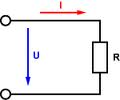
\includegraphics{images/ohmsche.jpeg}
		  	}
		  	\caption{Schaltplan einer einfachen U-I-Messung}
		  \end{figure}
		  
		
	Das Ohmsche Gesetz liefert hierfür:
	\begin{gather*}
		U=R\cdot I
	\end{gather*}
	Gesucht ist der zugehörige Widerstand $R$.\\
	
			  \begin{figure}
			  	\parbox{\linewidth}{
			  		\centering
			  		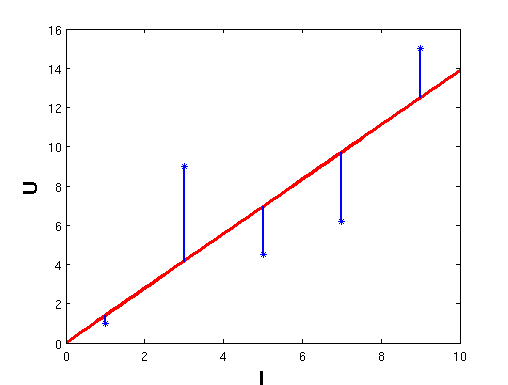
\includegraphics[width=0.5\linewidth]{images/linausgl2.png}
			  	}
			  	\caption{Linearausgleich einer U-I-Messung mit Ursprungsgerade als Modellfunktion}
			  \end{figure}
	
	
	Wird jetzt davon ausgegangen dass die $I_i$ exakt sind, wird das $R$ gesucht, 
	für das $RI_i$ im Mitttel den minimalen Abstand zu $U_i$ hat.
	Genauer gesagt berechne
	\begin{gather*}
		\min_{r\in\R} \sum_{i=1}^{m}(U_i-rI_i)^2
	\end{gather*}
	\textbf{Vorsicht: } Es wird \textbf{nicht} die Gerade (bzw. der lineare Untervektorraum) mit 
	minimalem euklidischem Abstand zu $(I_i,U_i)$ gesucht! \\
	Dieses Problem ist nichtlinear und aufwendig zu lösen.\\
	

	
	\subsection{Lineares Ausgleichsproblem} \index{Ausgleichsproblem!linear}
	Gegeben seien Messdaten $(t_i, b_i)$ mit $t_i, b_i\in \R$ für $i=1, \dots, m$ 
	und die Abhängigkeit $b(t)$ werde beschrieben durch eine Modellfunktion,
	 welche linear von den unbekannten Parametern $x_1, \cdots, x_n$ des Modells abhängt,
	 d.h.
	 \begin{gather*}
	 	b(t) = a_1(t)x_1 + \dots + a_n(t) x_n
	 \end{gather*}
	Für exakte Messdaten $b_i$ würde 
	\begin{gather*}
		b(t_i) = b_i \quad \forall i\in\{1,\cdots , m\}
	\end{gather*}
	gelten.\\
	Im Allgemeinen werden jedoch $m\geq n $ Messwerte $b_i$ bestimmt,
	und hiermit die $n$ Parameter $x_i$ so gewählt, dass die kleinsten
	\textbf{Fehlerquadrate auftreten}:
	\begin{gather}
		\min_{x_1, \dots x_n} \sum_{i=1}^{m} (b_i-b(t_i))^2 \label{IV.3.1}
	\end{gather}
	(Nach Gauß kann \eqref{IV.3.1} auch aus der Maximum-Likelihood-Methode\index{Maximum-Likelihood-Methode}
	für einen stochastischen Ansatz hergeleitet werden.)\\
		
	Definiere:
	\begin{align*}
		b &= (b_i)_{i=1,\dots, m}\in \R^m \\
		x &= (x_j)_{j=1,\dots, n}\in \R^n \\
		A &= (a_j(t_i)) _{\substack{i=1,\dots, m \\ j= 1, \dots, n}} \in \R^{m\times n}
	\end{align*}
	Damit ist \eqref{IV.3.1} äquivalent zum \textbf{linearen Ausgleichsproblem}:\\
	Zu gegebenem $b\in\R^m$ und $A\in\R^{m\times n}$ mit $m\geq n$
	ist das $\overline{x} \in \R^n$ gesucht mit 
	\begin{gather}
		\nn{b-A\overline{x}}_2 = \min_{x\in\R^n} \nn{b-Ax}_2
		\label{IV.3.2}
	\end{gather}
	Das entspricht der \enquote{Lösung} eines überbestimmten, i.A. nicht erfüllbaren
	GLS $Ax=b$.\\
	Aufgrund der $l_2$-Norm ist $\overline{x}$ gegeben durch die 
	orthogonale Projektion von $b$ auf den Bildraum $R(A) $ \index{Bildraum}, wie gleich gezeigt wird. \\
	
	IMAGE~MISSING\\
	
	\subsection{Projektionssatz} \index{Projektionssatz} \label{4.3.3}
	Sei $V$ ein reeller Vektorraum mit einem Skalarprodukt $\scp{\cdot}{\cdot}$
	und der induzierten Norm $\nn{v}\coloneqq \sqrt{\scp{v}{v}}$.
	Sei $U\subset V$ ein endlich dimensionaler Untervektorraum und sei
	\begin{gather*}
		U^\bot \coloneqq \left\{ v\in V  \, \middle\vert \, \scp{v}{u} = 0 ~~ \forall u\in U \right\}
	\end{gather*}
	Dann gilt:
	\begin{enumerate}[1)]
		\item Zu jedem $v\in V$ existiert genau ein $\overline{u}\in U$, 
		so dass $v-\overline{u}\in U^\bot$, d.h.
				\begin{gather*}
					\scp{v-\overline{u}}{u} = 0 \quad \forall u \in U
				\end{gather*}
		Dies definiert die \textbf{orthogonale Projektion} \index{orthogonale Projektion}
		\begin{gather*}
			P:V\rightarrow U, \quad v\mapsto \overline{u}= Pv
		\end{gather*}
		\item Zu jedem $v\in V $ bestimmt $P\cdot v$ die eindeutige Lösung
		\begin{gather*}
			\nn{v-Pv}= \min_{u\in U} \nn{v-u}
		\end{gather*}
		Also gilt mit einem eindeutigen $\overline{u}= Pv$, dass 
		\begin{gather}
			\nn{v-\overline{u}} = \min_{u\in U} \nn{v-u} 
			\Longleftrightarrow \scp{v-\overline{u}}{u} = 0 \quad \forall u\in U
			\label{IV.3.3}
		\end{gather}
	\end{enumerate}
	
	\begin{proof}
	\begin{enumerate}[1)]
		\item Sei $\{u_1, \dots , u_n \}$ eine Orthonormalbasis von $U$ 
		und $\overline{u}\in U $. \\
		Daraus folgt:
		\begin{gather*}
			\exists ! \, (\alpha_i)_{i=1,\dotsc,n} \subset \R: \overline{u} = \sum_{i=1}^{n} \alpha_i u_i
		\end{gather*}
		Damit gilt:
		\begin{alignat*}{3}
			&&0 &= \scp{v-\overline{u}}{u} &\quad& \forall u \in U \\
			&\Longleftrightarrow \quad& 0 &= \scp{v- \sum_{i=1}^{n} \alpha_i u_i}{u_i} &\quad &\forall j=1, \dots , n\\
			&\Longleftrightarrow  & \scp{v}{u_j} &= \sum_{i=1}^{n} \alpha_i \scp{u_i}{u_j} = \alpha_j
		\end{alignat*}
		Setze also 
		\begin{align}
		\nonumber
			P\cdot v &= \overline{u} \\
						& = \sum_{i=1}^{n} \scp{v}{u_i} u_i \in U
						\label{IV.3.4}
		\end{align}
		dann ist $\overline{u}$ die eindeutig bestimmte Lösung für $ v-\overline{u} \in U^\bot$
		
	 IMAGE~MISSING \\
		
			Sei  $u\in U$. Dann gilt:
			\begin{align}
			\nonumber
				\nn{v-u}^2 &= \nn{v-\overline{u}+\overline{u} -u}^2 \\ \nonumber
								   &= \nn{v-\overline{u}}^2 +
								          \underbrace{\scp{v-\overline{u}}{\overbrace{\overline{u}-u}^{~~\in U}}}_{=0}
								          + \nn{u-\overline{u}}^2 \\
								   &= \nn{v-\overline{u}}^2 + \nn{u-\overline{u}}^2
								   \label{IV.3.5}
			\end{align}
			(Dies ist anschaulich der Satz des Pythagoras.)
	\end{enumerate}
	\end{proof}
	
	\subsection{Satz} 
	Der Vektor $\overline{x} \in\R^n$ ist genau dann Lösung des linearen Ausgleichsproblems
	\begin{gather*}
		\min_{x\in\Ren} \nn{b-Ax}_2 \, ,
	\end{gather*}
	falls er die Normalengleichung
	\begin{gather}
		A^TA\overline{x} = A^Tb
		\label{IV.3.6}
	\end{gather}
	erfüllt. \\
	Insbesondere ist $\overline{x}$ eindeutig,
	falls $A\in \R^{m\times n}$ maximalen Rang $n\leq m$ hat.
	
	\begin{proof} Bezeichne
	 $V= \R^m, U= R(A) = \left\{Ax \, \middle|  \, x \in\Ren \right\}, b \in \R^m$.\\
	 Nach \eqref{IV.3.3} gilt:
	 \begin{alignat*}{2}
	 	&&\nn{b-A\overline{x}}_2 &= \min_{x\in\Ren} \nn{b-Ax}_2 \\
	 	&\Leftrightarrow \quad & \scp{b-A \overline{x}}{Ax} &= 0 \quad \forall x\in \Ren \\
	 	&\Leftrightarrow & \scp{A^T(b-A\overline{x})}{x} &= 0 \quad  \forall x\in\Ren \\
	 	&\Leftrightarrow & A^T(b-A\overline{x}) &= 0 \\
	 	&\Leftrightarrow & A^TA\overline{x} &= A^Tb
	 \end{alignat*}
	 Nach dem Projektionssatz \ref{4.3.3} existiert mindestens ein eindeutiges
	 $\overline{y} = P b$.
	 Für dieses $\overline{y}$ ist $\overline{x}\in \Ren $ mit $\overline{y} = A\overline{x}$
	 eindeutig bestimmt, falls $A$ injektiv ist, d.h. falls $rang(A) = n$. \end{proof}
	 
	 
	 Ähnlich zum Skalarprodukt ist die relative Kondition von $(P,b) $ schlecht, 
	 falls $b$ fast senkrecht zu $U$ steht.
	 Die relative Kondition des linearen Ausgleichsproblems hängt zusätzlich von $cond(A)$ ab.
	 
	 
	 \subsection{Lösung der Normalgleichung}
	 Falls $rang(A) = n$, ist $A^TA$ spd und das Cholesky-Verfahren ist anwendbar. \\
	 Dafür ist
	 \begin{enumerate}[1.]
	 	\item $A^TA$ zu berechnen:
		 	\begin{description}
		 		\item[Aufwand] ca. $\frac{1}{2}n^2m$ Multiplikationen 
		 		\item[Kondition] häufig schlecht, da $\frac{1}{2}n^2$ Skalarprodukte berechnet werden
		 	\end{description}
	 	\item die Cholesky-Zerlegung von $A^TA $ durchzuführen:
		 	\begin{description}
		 		\item[Aufwand] ca. $\frac{1}{6}n^3$ Multiplikationen 
		 		\item[Kondition] Für $A\in\R^{m\times n}$ mit $m\geq n$ und $rang(A)=n$ gilt:
		 								\begin{gather}
		 									cond_2(A^TA) = cond_2(A)^2 \label{IV.3.7}
		 								\end{gather}
		 								(siehe Übungsaufgabe 19)
		 	\end{description}
	 \end{enumerate}
	 			Also überwiegt für $m\gg n$ der Aufwand $A^tA$ zu berechnen.
	 			Die auftretenden Konditionen entsprechen i.d.R. nicht dem des Ausgangsproblems.\\
	 			Damit ist die 
	 			\textbf{Cholesky-Zerlegung \index{Cholesky-Zerlegung} für Normalgleichungen ungeeignet}.
	 
	 
	 \subsection{Satz}
	 Sei $A\in \R^{m\times n} $ mit $m\geq n$ und $rang(A) = n$,
	 sei $b\in\R^m$ und besitze $A$ eine Zerlegung
	 \begin{gather*}
	 	A= Q\begin{pmatrix}R\\0\end{pmatrix}
	 \end{gather*}
	 mit einer orthogonalen Matrix $Q\in R^{m\times m}$ und 
	 einer oberen Dreiecksmatrix $R\in \R^{n\times n}$. \\
	 Dann ist $R$ invertierbar. \\
	 Bezeichne 
	 \begin{gather}
	 	\begin{pmatrix} \overline{b}_1 \\ \overline{b}_2\end{pmatrix}
	 	\coloneqq Q^T\cdot b
	 	\label{IV.3.9}
	 \end{gather}
	 dann ist
	 \begin{gather}
	 	\overline{x} = R^{-1} \overline{b}_1 
	 	\label{IV.3.10}
	 \end{gather}
	 die Lösung des linearen Ausgleichsproblems und
	 \begin{align*}
	 	\nn{\overline{b}_2} &= \nn{b-A\overline{x}} \\
	 									& = \min_{x\in \Ren }\nn{b-Ax}
	 \end{align*}
	 Zur Erinnerung:
	 \begin{align*}
	 	Q \text{ orthogonal} &:\Leftrightarrow QQ^T = I \\
	 									&\, \Leftrightarrow Q^{-1} = Q^T
	 \end{align*}
	 Weiterhin ist $Q$ längenerhaltend\index{längenerhaltend}, d.h. $\nn{Qv}_2 = \nn{v}_2$ 
	 und somit folgt
	 \begin{gather}
	 \nonumber
	 	\nn{Q}_2 = \nn{Q^{-1}}_2 = 1 \quad \text{und} \\
	 	cond_2(Q) = 1
	 	\label{IV.3.11}
	 \end{gather}
	 
	 \begin{proof} $R$ ist invertierbar, da 
	 \begin{align*}
	 	rang(R) &= rang(Q^{-1}\cdot A) \\	
	 				& = rang(A) \\
	 				&= n
	 \end{align*}
	 Außerdem gilt:
	 \begin{align*}
	 	\nn{b-Ax}_2^2 & = \nn{Q(Q^Tb-\begin{pmatrix}R\\0\end{pmatrix}x)}_2^2 \\
	 							&=  \nn{Q^Tb-\begin{pmatrix}Rx\\0\end{pmatrix}}_2^2  \\
	 							&\overset{\mathllap{\text{$Q$ längenerhaltend}}}{=}
	 							   \nn{\overline{b}_1 - Rx}_2^2  + \nn{\overline{b}_2^2}
	 \end{align*}
	 wird minimal für $R\overline{x} = \overline{b}_1$
	\end{proof}
	 
	 Da $Q$ längenerhaltend ist, folgt mit \ref{3.2.13} b)
	 ($cond_A \coloneqq \frac{\max \nn{Ax}}{\min \nn{Ax}}$)
	 sofort:
	 \begin{gather*}
	 	cond_2(A) = cond_2(R)
	 \end{gather*}
	Die auftretende Kondition entspricht also der des Ausgleichsproblems.
	
	
	\subsection{Bemerkung}
	Sei $A\in \Renn$ invertierbar und habe ein QR-Zerlegung, d.h. es existiert
	eine orthogonale Matrix $Q$ und eine obere Dreiecksmatrix $R$, so dass:
	\begin{gather*}
		A= Q\cdot R
	\end{gather*}
	Dann kann das Gleichungssystem $Ax=b$ wie folgt gelöst werden:
	\begin{enumerate}[1.]
		\item Setze $z=Q^Tb$, was Kondition 1 hat.
		\item Löse durch Rückwärtssubstitution $Rx=z$.
	\end{enumerate}
	
		
\marginpar{12.11.2014}

\sectione{Orthogonalisierungsverfahren}		\index{Orthogonalisierung}
Konsturiere eine QR-Zerlegung
\begin{gather}
	A= Q\cdot \begin{pmatrix} R\\0 \end{pmatrix}
	\label{IV.4.1}
\end{gather}
	durch einen Eliminationsprozess:
	\begin{gather}
		A \rightarrow Q^{(1)}A \rightarrow Q^{(2)} Q^{(1)}A \rightarrow Q^{(p)}\cdot \dotsc \cdot Q^{(1)}A
		= \begin{pmatrix} R\\0 \end{pmatrix}\, .
		\label{IV.4.2}
	\end{gather}
	mit orthogonalen Matrizen $Q^{(i)}$.
	Dann gilt
	\begin{gather}
		Q= Q^{(1)T}\cdot \dotsc \cdots {Q^{(p)T}}
		\label{IV.4.3}
	\end{gather}
	Dies ist im Gegensatz zur $LR$-Zerlegung aufgrund von $cond(Q^{(i)})= 1$ immer stabil.\\
	
	Für $Q\in\R^{2\times 2}$ gibt es zwei mögliche Anschauungen, nämlich:
	\begin{enumerate}[a)]
		\item Drehung ~~~ IMAGE~MISSING
		\item Spiegelung ~~~ IMAGE~MISSING
	\end{enumerate}
	
	\extrasection{a)}{Givens-Rotation}
	Es wird eine Drehung auf den 1. Einheitsvektor durchgeführt:\\
	
	IMAGE~MISSING\\
	
	\begin{gather*}
		a=\begin{pmatrix}a_1 \\ a_2\end{pmatrix} \rightarrow \begin{pmatrix}\alpha \\ 0 \end{pmatrix}
		= \alpha e_1
	\end{gather*}
	d.h. Elimination von $a_2$ mit
	\begin{gather*}
		\nn{\alpha e_1}_2 = \nn{a}_2
	\end{gather*}
	Also gilt für $\alpha$
	\begin{gather*}
		\alpha=\pm \nn{a}_2
	\end{gather*}
	Drehuungen werden beschrieben durch
	\begin{gather*}
		Q = \begin{pmatrix}
					cos(\theta) & sin(\theta)\\
					-sin(\theta) & cos(\theta)
				\end{pmatrix}
		\eqqcolon \begin{pmatrix}
								c & s\\
								-s & c
						\end{pmatrix}\qquad \theta \in[0,2\pi)
	\end{gather*}
	und es muss gelten
	\begin{gather*}
		Qa = \begin{pmatrix}\alpha \\ 0 \end{pmatrix}
	\end{gather*}
	Hiermit folgt für $\nn{a}= 0$
	\begin{align}
	\nonumber
		c&=1, s=0\\ \nonumber
		c&=\frac{a_1}{\alpha},  s= \frac{a_2}{\alpha}\quad \text{mit}\\
		\alpha & = \pm \sqrt{a_1^2+a_2^2}
		\label{IV.4.4}
	\end{align}
	für $\nn{a}\neq 0$.\\
	Im Folgenden wird dies kurz mit
	\begin{gather*}
		[c,s] = givens(a_1, a_2)
	\end{gather*}
	bezeichnet. \\
	Als \textbf{Givens-Rotation}\index{Givens-Rotation} wird eine Matrix der Form
	\begin{gather}
		\Omega _{k,l} = \begin{pmatrix}
										1 &&&&&&&&& \\
										& \ddots\\
										&& 1\\
										&&& \mathbf{c} &&&& \mathbf{s} \\
										&&&& 1\\
										&&&&& \ddots \\
										&&&&&& 1\\
										&&& -\mathbf{s} &&&& \mathbf{c} \\
										&&&&&&&& \ddots \\
										&&&&&&&&& 1\\
									\end{pmatrix}
									 \begin{array}{l}
									 \\   \leftarrow \text{$k$-te Zeile}
									 \\ \\ \\ \\ \leftarrow \text{$l$-te Zeile}
									 \end{array}
									 \label{VI.4.5}
	\end{gather}
	mit $c^2+s^2=1$ und $k<l$ bezeichnet.\\
	Es folgt:
	\begin{align*}
		\Omega_{kl} A &= \widetilde{A} \quad \text{mit} \\
		\widetilde{a}_{ij}  &= a_{ij} \quad \text{ für } i\neq k,l \\
		\widetilde{a}_{kj} & = ca_{kj}+sa_{lj} \\
		\widetilde{a}_{lj} & = -sa_{kj} + ca_{lj}
	\end{align*}
	Demnach werden nur die $k$-te und $l$-te Zeile werden verändert. \\
	Falls nun $[c,s] = givens(x_k, x_l)$ gilt
	\begin{gather*}
		\Omega_{k,l}\cdot x = \begin{pmatrix}
		x_1 \\ \vdots \\x_{k-1} \\\alpha \\ x_{k+1}
		\\\vdots \\
		x_{l-1} \\ 0 \\x_{l+1} \\\vdots \\x_n
		\end{pmatrix}
		\qquad
		\quad \text{mit~~}
		\alpha = \pm \nn{  \begin{pmatrix} x_k \\ x_l\end{pmatrix}}_2
	\end{gather*}
	d.h. eine Givens-Rotation erzeugt eine Null.\\
	Da nun
	\begin{gather*}
		\R^{m\times n}\ni \begin{pmatrix}
		* & * &* & \dots   \\
		0 & * &     \\
		0 & 0 & \ddots \\
		\vdots \\
		0 & 0 & 0 & \dots & *		
		\end{pmatrix}
		= \begin{pmatrix} R\\0\end{pmatrix}
	\end{gather*}
	gilt, sind
	\begin{gather*}
		p=\sum_{j=1}^{n}(m-j)
	\end{gather*}
	Givens-Rotationen nötig, um eine QR-Zerlegung nach \eqref{IV.4.1} zu erzeugen.
	Und eine Rotation, welche $a_{ij} $ auf 0 setzt, ist durch zugehörige 
	$(c_{ij}, s_{ij}) $ gegeben.\\
	
	Für eine 3x4-Matrix sieht das Verfahren folgendermaßen aus:
	
	\begin{align*}
		A= &
		\left(\begin{array}{lccc}
			*~ &&&\\
			* &&* \\
			* \rcurvearrownw \\ * \lcurvearrowsw
		\end{array}\right)
		\quad \overset{\Omega_{3,4}}{\longrightarrow} \quad
		\left(\begin{array}{lccc}
			*~ &&&\\
			* \rcurvearrownw && *\\
			* \lcurvearrowsw \\
			0
		\end{array}\right)
		\quad \overset{\Omega_{1,2}}{\longrightarrow} \quad
		\left(\begin{array}{lccc}
		* \rcurvearrownw\\
		* \lcurvearrowsw && *& \\
		0 \\
		0
		\end{array}\right)\\
		\quad \overset{\Omega_{2,3}}{\longrightarrow} \quad
		&\left(\begin{array}{lccc}
			*~~ \\
			0 && *&~ \\
			0 \\
			0
		\end{array}\right)
		\quad \overset{\Omega_{3,4}}{\longrightarrow} \quad	
		\left(\begin{array}{clcc}
			* & *\\
			0 & *  \rcurvearrownw  & *& \\
			0 & * \lcurvearrowsw \\
			0 & 0
		\end{array}\right)
		\quad \overset{\Omega_{2,3}}{\longrightarrow} \quad	
		\left(\begin{array}{cccl}
			* & *  & * \\
			0 & *  & * \\ 
			0 & 0 & * \rcurvearrownw\\
			0 & 0 & *  \lcurvearrowsw 
		\end{array}\right) \\
		\quad \overset{\Omega_{3,4}}{\longrightarrow} \quad	
		& \left(\begin{array}{cccc}
		* & *  & *  \\
		0 & *  & * \\ 
		0 & 0 & * \\
		0 & 0 & 0
		\end{array}\right)
		= \begin{pmatrix}
			R \\ 0 
		\end{pmatrix}
	\end{align*}

	
	Es ergibt sich:
	
	\subsection{Givens-QR-Algorithmus} \index{Givens-QR-Algorithmus}
	
	\begin{pseudocode}{0.7\linewidth}
		\textbf{for} $j=1, \dotsc , n$ \\
		|~	\>	\textbf{for} $i=m, m-1, \dotsc , j+1$ \\
		|~	\>		|~	\>\% \textit{setze $a_{ij}$ auf 0} \\
		|~	\>		|~	\>$[c,s] = givens(a_{i-1,j}, \dotsc, a_{ij}) $\\
		|~	\>		|~	\>speichere $c$ und $s$ für $a_{ij}$ \\
		|~	\>		|~	\>$A(i-1:j, j:h) =\left( \begin{smallmatrix}c & s\\ -s & c	\end{smallmatrix}\right) * A(i-1:j, j:n)$ \\
		|~	\> \textbf{end}\\
		\textbf{end}							
	\end{pseudocode}
	
	\subsection{Bemerkungen} 
	\begin{enumerate}[a)]
		\item $A(i-1 : i, 1 : j-1) = 0$ und ist daher nicht zu berechnen oder
					zu speichern. Der Speicherplatz kann für die Speicherung der
					Givensrotationen benutzt werden.
		\item  $R$ steht anschließend in $A$.
		\item Die Bestimmung der Länge $|\alpha|$ wird so ausgeführt, dass over- ¨
				oder underflow vermieden wird. Weiterhin wird das Vorzeichen
				von $c$ oder $s$ festgelegt, so dass aufgrund von $c^2+s^2=1$ nur
				ein Wert $\rho$ gespeichert werden muss. Hiermit wird auch das
				Vorzeichen von $\alpha$ festgelegt:\\
				\begin{description}
					\item[$a_2=0$:] Setze $c=1, s=0, \alpha = a_1$, merke $\rho=1$.
					\item[$|a_2|>|a_1|$:] Setze $\tau= \frac{a_1}{a_2}, s=\frac{1}{\sqrt{1+\tau^2}}, c=s\cdot\tau, \alpha =a_2\sqrt{1+\tau^2}$, merke $\rho=\frac{c}{2}$.
					\item[$|a_1|\geq|a_2|$:] Setze $\tau= \frac{a_2}{a_1}, c=\frac{1}{\sqrt{1+\tau^2}}, s=c\cdot\tau, \alpha =a_1\sqrt{1+\tau^2}$, merke $\rho=\frac{2}{s}$.
				\end{description}
		\item Aufgrund von c) muss nur $\rho$ gespeichert werden:
		\begin{description}
			\item[$\rho=1$:] Setze $c=1, s=0$.
			\item[$|\rho|<1$:] Setze $c=2\rho , s= \sqrt{1-c^2}$.
			\item[$|\rho|>1$:] Setze $s=\frac{2}{\rho}, c=\sqrt{1-s^2}$.
		\end{description}
	\end{enumerate}
	Hiermit können alle notwendigen Givens-Rotationen als untere
	Dreiecksmatrix zusammen mit $R$ in $A$ gespeichert werden.
	
	
	
	\subsection{Aufand des Givens-QR-Algorithmus}
	\begin{enumerate}[a)]
		\item $m\approx n$\\ $\rightarrow $  ca. $\frac{4}{3}n^3$ Multiplikationen
				und $\frac{1}{2}n^2$ Quadratwurzeln nötig \\
				Die Givens-QR-Zerlegung ist somit ungefähr viermal so aufwändig
				wie die Gauß-Elimination, dafür jedoch stabil.
		\item $m\gg n$\\ $\rightarrow $ ca. $2n^2m$ Multiplikationen und 
				$mn$ Quadratwurzeln nötig \\
				Das Verfahren ist daher zwei- bis viermal so aufwändig wie das
				Cholesky-Verfahren für die Normalgleichungen, aber stabil.
		\item Bei Hessenberg-Matrizen, d.h. Matrizen mit der Gestalt
				\begin{gather}
					A= \begin{pmatrix}
						* & \dots&& * \\
						*&* \\
					    &\ddots& \ddots \\
					     \\
					    0 &&& * 
					\end{pmatrix}
					\label{IV.4.7} \, ,
				\end{gather}
				also $a_{ik} = 0 \forall i<k+1$,
				sind nur $(n-1)$ Givens-Rotationen auszuführen. \\
				Diese Matrizen tauchen z.B. bei Eigenwertberechungen auf
				 und sind dort ein wichtiger Bestandteil der Verfahren.
	\end{enumerate}
	
	
	\extrasection{b)}{Householder-Reflexion}
	
	Es sei $H$ eine Hyperebene im $\R^m$ und zusätzlich ein Vektor $a\in\R^m$ gegeben. \\
	
	IMAGE~MISSING \\
	
	Gesucht ist nun die Reflexion $Q$, so dass
	\begin{gather*}
		Qa = \alpha e_1 = \begin{pmatrix} \alpha \\ 0\\\vdots\\0\end{pmatrix}
		\qquad \text{mit } \alpha = \pm \nn{a}
	\end{gather*}
	Mit \begin{gather}
		v=a-\alpha e_1 
		\label{IV.4.8}
	\end{gather}
	gegeben, welches senkrecht zu $H$ steht.\\
	Damit Stellenauslöschungen in $v$, d.h. in $v_1$, vermieden werden,
	wähle ein entsprechendes Vorzeichen für $\alpha$, also 
	\begin{gather}
		\alpha = -sign(a_1)\nn{a}_2 
		\label{IV.4.9}
	\end{gather}
	Die zugehörige Reflexion $Q$ ist  gegeben durch \\
	
	IMAGE~MISSING \\
	
	wobei
	\begin{align}
	\nonumber
		w &= \scp{\frac{v}{\nn{v}}}{x} \cdot \frac{v}{\nn{v}} \\ %\nonumber
		Qx &= x-2w = x-2\frac{v^Tx}{v^Tv}v 
			 = (I-2\frac{vv^T}{v^Tv})x 
			 \label{VI.4.10}\\
	    Q  &= I-2\frac{vv^T}{v^Tv}&& vv^T \in \Renn,\,\, v^Tv\in\R
	    	\label{VI.4.11}
	\end{align}
	und heißt \textbf{Householder Reflexion} \index{Householder Reflexion}
	 (wurde  1958 von Householder eingeführt).  \\
	 Für die spezielle Wahl \eqref{IV.4.8} mit \eqref{IV.4.9} vom Vektor $v$ folgt
	 \begin{align}\nonumber
	 	vv^T = \nn{v}^2 &= \nn{a}^2 - 2\alpha\scp{a}{e_1} + \alpha^2 \\ \nonumber
	 	&= -2\alpha(a_1-\alpha) \\
	 	& = -2\alpha v
	 	\label{IV.4.12}
	 \end{align}
	
	
	 \subsection{Bemerkung}\label{4.4.4}
	 \begin{enumerate}[a)]
	 	\item Q ist symmetrisch
	 	\item Q ist orthogonal
	 	\item Q ist involutorisch, d.h. $Q^2 = I$ ~~(bzw. gilt $Q^{-1}= Q^T=Q$)
	 \end{enumerate}
	 Die Householder Reflexion setzt nicht nur eine Null,
	  sondern im Vektor gleich alle gewünschten Nullen
	  \begin{align*}
	  	\text{\textbf{Rotation: }}&
	  	\quad \begin{pmatrix} * \\ * \\ *	\end{pmatrix}
	  	\rightarrow \begin{pmatrix} * \\ * \\0	\end{pmatrix}
	  	\rightarrow \begin{pmatrix} * \\0\\0	\end{pmatrix} \\
	  	\text{\textbf{Reflexion: }}&
	  	\quad \begin{pmatrix} * \\ * \\ *	\end{pmatrix}
	  	\rightarrow \begin{pmatrix} *\\0\\0	\end{pmatrix}
	  \end{align*}
	  Um die erste Spalte in $A$ auf die gewünschte Gestalt zu bringen,
	  bestimme $Q^{(1)}$ wie oben, indem die erste Spalte als $a$ gewählt wird:
	  \begin{gather*}
	  	A\rightarrow A^{(1)} = Q^{(1)} A =
	  	\begin{pmatrix}
	  		\alpha^{(1)} \\
	  		0 &*&~~\\
	  		\vdots \\
	  		0
	  	\end{pmatrix}
	  \end{gather*}
	  In der $k$-ten Spalte sollen nun die $(k-1)$-ten Zeilen und die $(k-1)$-ten Spalten
	  bleiben und die Restmatrix verändert werden.\\
	  
	 \begin{align*}
	 A^{(k-1)} &=
	 \begin{pmatrix}
	 *  &&&&&\\
	 &\ddots &&&& * \\
	 &&*&&\_&\_&\_ \\
	 &&0&|&\\
	 &0&\vdots&| &&T^{(k-1)}\\
	 &&\vdots&  |\\
	 &&0&  |
	 \end{pmatrix}
	 \begin{array}{l}
	 \\
	 \shortleftarrow (k-1) \text{-te Zeile} \\
	 \\\\\\\\
	 \end{array}\\
	 &\phantom{= \, (} \begin{array}{ccl}
	 	~&~&~ \uparrow (k-1)\text{-te Spalte}
	 \end{array}
	 \end{align*}
	  
	  Setze also
	  \begin{gather}
	  	Q^{(k)} = \begin{pmatrix}
	  	 I_{k-1} & 0 \\
	  	 0 & \overline{Q}^{(k)} \, ,
	  	 \label{IV.4.13}
	  	\end{pmatrix}
	  \end{gather}
	  wobei $\overline{Q}^{(k)} $ durch die erste Spalte von $T^{(k)}$, d.h.
	  \begin{gather}
	  	a= (a_{i,k}^{k-1})_{i=k,\dotsc, m} \subset \R^{m+1-k}
	  	\label{IV.4.14}
	  \end{gather}
	  bestimmt wird. Dann gilt
	  \begin{gather*}
	  	Q^{(k)}A^{(k-1)} =
	  	 \begin{pmatrix}
	  	*  &&&&&\\
	  	&\ddots &&&& * \\
	  	&&*&&\_&\_&\_&\_ \\
	  	&&0&|&* \\
	  	&0&\vdots&|&0&* \\
	  	&&\vdots&  |&\vdots &&\ddots\\
	  	&&0&  |&0&&&*
	  	\end{pmatrix}
	  \end{gather*}
	  Nach insgesamt 
	  \begin{gather}
	  	p=\min (m-1, n)
	  	\label{IV.4.15}
	  \end{gather}
	  Schritten erhalten wir für $A\in \R^{m\times n}$
	  \begin{gather}
	  Q^TA = Q^{(p)}\cdot \dotsc \cdot Q^{(1)}A 
	  			= \begin{pmatrix} R\\0\end{pmatrix}\, ,
	  \end{gather}
	  wobei Bemerkung \ref{4.4.4} auch für 
	  $Q^T= Q^{(p)}\cdot \dotsc \cdot Q^{(1)} $ und somit auch für
	  \begin{gather}
	  	Q = Q^{(1)}\cdot \dotsc \cdot Q^{(p)}
	  	\label{IV.4.16}
	  \end{gather}
	  gilt.
	  
	  
	  
\marginpar{17.11.2014}

	\subsection{Speicherung}
	Gespeichert werden müssen die obere Dreiecksmatrix $R$ und die 
	\textbf{Householdervektoren} \index{Householdervektoren}
	$v^{(i)}\in \R{m+1-i}$.
	Die Diagonalelemente von $R$ sind $r_{ii} = \alpha^{(i)}$. \\
	Folgende Speicheraufteilung ist möglich:
	\begin{gather*}
		A \longrightarrow \left(
		\begin{array}{rrrrr}
			|&&& R \\
			|&| \\
			v^{(1)}| & v^{(2)}|&\ddots ~~\\
			| &|&\phantom{v^{(i)}}|& v^{(p)}			
		\end{array}
		\right)
		\quad \text{und} \quad 
		\begin{pmatrix}
			\alpha^{(1)} \\ \vdots \\ \\ \alpha^{(p)}
		\end{pmatrix}
	\end{gather*}
	  
	  Wohlgemerkt kann so auch $A\in \R{m\times n}$ mit $m<n$ bearbeitet werden,
	  dann wird $A$ zu:
	  
	  \imagemissing{Zerlegung einer mxn-Matrix für $m<n$}
	  
	  Falls zusätzlich $v^{(i)}$ so normiert ist,
	  dass $v_1^{(i)} = 1$ ist, braucht diese Komponente nicht gespeichert werden 
	  und $R$ kann komplett in $A$ gespeichert werden.
	  
	  \subsection{Aufwand für den Householder-QR-Algorithmus}
	  \begin{enumerate}[a)]
	  	\item Falls $m\approx n$ sind ungefähr $\frac{2}{3}n^3$ Multiplikationen notwendig
	  	und ist somit ungefähr doppelt so teuer wie die LR-Zerlegung, ist aber stabil.
	  	\item Falls $m\gg n$ sind ungefähr $2mn^2$ Multiplikationen notwendig.
	  	Der Aufwand ist daher ungefähr so hoch wie beim Cholesky-Verfahren für Normalgleichungen,
	  	aber stabil.
	  \end{enumerate}
	  
	  
	  \chapter{Numerische Lösung nichtlinearer Gleichungssysteme}
	  Beispiel:\\
	  linear: $Ax=b$ \\
	  nichtlinear: $f(x) = \sin(x) +x^3-4=0$
	  
	  \sectione{Einführung}
	  \subsection{Beispiele}
	  \begin{enumerate}[1)]
	  	\item $f(x) = x^2-c = 0 \Leftrightarrow x= \pm \sqrt{c}$: \\Berechnung der Wurzel
	  	\item Sei $p$ ein Polynom:\\ Nullstellenbestimmung
	  	\item Löse das nichtlineare Randwertproblem
	  			\begin{gather*}
	  				-\Delta u = f(u)
	  			\end{gather*}
	  			in $\Omega=(0,1)^2$ mit $u=0$ auf $\partial \Omega$. \\
	  			Mit dem Differenzenverfahren\footnote{s. Übungsaufgabe 2)}
	  			ergibt sich
	  			\begin{gather*}
	  				A\vec{u} = h^2 \vec{f}(\vec{u})
	  			\end{gather*}
	  			ein System nichtlinearer Gleichungen.
	  \end{enumerate}
	  
	  \subsubsection{Nullstellenbestimmung}\index{Nullstellenbestimmung}
	  \begin{description}
	  	\item[Gegeben]   $D\subseteq \R^n, f: D\rightarrow \R^m$ stetig
	  	\item[Gesucht]    $x^{*}\in D $ mit $f(x^{*}) = 0$
	  \end{description}
	
	\subsubsection{Fixpunktgleichung}\index{Fixpunktiteration}
	  	  \begin{description}
	  	  	\item[Gegeben]   $D\subseteq \R^n, g: D\rightarrow \R^n$ stetig
	  	  	\item[Gesucht]      $x^{*}\in D $ mit $g(x^{*}) = x^{*}$
	  	  \end{description}
	  	  Falls m=n ist dies äquivalent zur Nullstellenbestimmung.
	  	  
	  \subsection{Das Bisektionsverfahren}\index{Bisektionsverfahren}
	  Sei $f:[a,b]\rightarrow \R $ stetig udn$f(a) \cdot f(b) <0$.\\
	  Dann folgt aus dem Zwischenwertsatz die Existenz
	  mindestens einer Nullstelle $x^{*}\in (a,b)$.
	  
	  \imagemissing{Beispiel zur Nullstellenexistenz}
	  
	  Generiere eine Folge von Intervallen
	  $[a^{(i)}, b^{(i)}]\in  [a^{(i-1)}, b^{(i-1)}] $,
	  die eine Nullstelle enthalten und mit $b^{(i)}-a^{(i)} \longrightarrow 0$.
	  Definiere
	  \begin{gather}
	  	x^{(i+1)}= \frac{1}{2}(b^{(i)}+a^{(i)})
	  	\label{V.1.1}
	  \end{gather}
	  und
	  \begin{gather}
	  	[a^{(i+1)}, b^{(i+1)}] \coloneqq \begin{cases}
	  		 [x^{(i+1)}, b^{(i)}] & \text{für } f(a^{(i)})\cdot f(x^{(i+1)}) > 0 \\
	  		 [a^{(i)}, x^{(i+1)}] & \text{für } f(a^{(i)})\cdot f(x^{(i+1)}) < 0
	  	\end{cases}
	  	\label{V.1.2}
	  \end{gather}
	  Für jedes $i\geq 1$ gilt somit
	  \begin{gather*}
	  	b^{(i)}-a^{(i)} = \frac{1}{2^i}(b-a)
	  \end{gather*}
	  und es existiert eine Nullstelle $x^{*}$ in $[a^{(i)}, b^{(i)}]\in  [a^{(i-1)}, b^{(i-1)}] $
	  für alle $i$. \\
	  Damit folgt
	  \begin{align*}
	  	|x^{(i-1)}-x^{*}| &\leq \frac{1}{2}(b^{(i)}-a^{(i)}) \\
	  								&=  2^{-(i+1)} (b-a) \longrightarrow 0
	  \end{align*}
	  Also $\lim_{i\rightarrow \infty}x^{(i)} = x^{*}$.
	  
	  
	\subsection{Korollar}
	Das oben angegebene Bisektionsverfahren konvergiert, falls
	$f:[a,b]\rightarrow \R $ stetig ist und 
	$f(a)\cdot f(b) <0$ gilt.
	
	\subsection{Bemerkungen}
	\begin{enumerate}[a)]
		\item $x^{(i)} $ wird als Intervallmitte, also unabhängig von $f(x^{(i)})$
		gewählt. die Konvergenzgeschwindigkeit hängt von der Länge des Intervalls $[a,b]$ ab
		und der Lage von $x^{*}$ bezüglich der Intervallhalbierung ab. \\
		Die Konvergenz kann demnach sehr langsam sein.
		\item Ein Vorteil ist, dass keine Differenzierbarkeitsvoraussetzungen nötig sind.
		\item Das Verfahren ist nicht für $f:D\longrightarrow \R^n$ anwendbar.
	\end{enumerate}
	
	
	\sectione{Fixpunktiteration}\index{Fixpunktiteration}
	Gesucht sei ein Fixpunkt $x^{*}\in D\subseteq \R^n$ der stetigen Funktion
	$g:D\rightarrow\R^n$, d.h.
	\begin{gather}
		x^{*} = g(x^{*}) \label{V.2.1}
	\end{gather}
	\textit{Idee:}
	Nutze \eqref{V.2.1} zur Iteration, d.h. wähle $x^{(0)}\in D$,
	setze 
	\begin{gather}
		x^{(k+1)} = g(x^{(k)})  \quad \text{für } k\in 0, 1, \dotsc
		\label{V.2.2}
	\end{gather}
	Es bedarf noch der Voraussetzung, dass $x^{(k)}\in D~~ \forall k$ \\
	Falls $x^{(k)}$ konvergiert, ist der Grenzwert $x^{*}$ ein Fixpunkt,
	denn für stetiges $g$ gilt:
	\begin{align} \nonumber
		x^{*} = \lim_{k\rightarrow \infty}x^{(k+1)} &= \lim_{k\rightarrow \infty}g(x^{(k)}) \\
		     & \overset{\mathclap{g \text{ stetig}} }{=}\quad g(\lim_{k\rightarrow \infty}x^{(k)}) = g(x^{*})
		     \label{V.2.3}
	\end{align}
	
	\subsection{Beispiel}
	Löse $x-e^{-x}-1 = 0$.
	\begin{enumerate}[a)]
		\item $x=1+e^{-x} \eqqcolon g_1(x)$
		\imagemissing{Konvergenz der Fixpunktiteration für $x=1+e^{-x}$}\\
		$\longrightarrow$ Konvergenz
		\item $e^{-x} = x-1   \Leftrightarrow x= -ln(x-1) \eqqcolon g_2(x)$
		\imagemissing{Versagen der Fixpunktiteration für $x=-ln(x-1)$}\\
		$\longrightarrow$ $g(x^{(2)}) $ nicht definiert!
	\end{enumerate}
	
	\subsection{Definition: Kontraktion} \index{Kontraktion}
	Sei $D\subseteq  \R^n $ abgeschlossen und $\nn{\,\cdot\,}$ eine Norm auf dem $\R^n$.
	Eine Abbildung $g:D\rightarrow \R^n $ heißt \textbf{Kontraktion} bezüglich  $\nn{\,\cdot\,}$,
	falls es ein $\kappa \in [0,1)$ gibt mit
	\begin{gather*}
		\nn{g(u)-g(v)} \leq \kappa \nn{u-v} \quad \forall u,v\in D
	\end{gather*}
	Die kleinste solche Zahl $\kappa$ heißt Kontraktionszahl von g.
	
	\imagemissing{Grafische Veranschaulichung einer Kontraktion}
	
	Offensichtlich ist jede auf $D$ kontrahierende Abbildung stetig.
	
	\subsection{Lemma} \label{5.2.3}
	Sei $D=\overline{\Omega} $ mit $\Omega \subseteq \R^n$ offen und konvex
	und $\nn{\,\cdot\,}$ eine Norm auf dem $R^n$.\\
	Falls $g:D\longrightarrow \R^n$ eine stetig differenzierbare Funktion ist und
	bezüglich der zugeordneten Matrixnorm $\sup_{x\in \Omega}\nn{Dg(x)}<1$ gelte,
	so ist $g$ kontrahierend bezüglich  $\nn{\,\cdot\,}$.
	
	\begin{proof}
		Mit $u,v \in D$ gilt $u+t(v-u)\in D$, da $D$ konvex ist. \\
		Somit ist $h:[0,1]\rightarrow \R^n $ mit $h(t) \coloneqq g(u+t(v-u))$ wohldefiniert
		und stetig differenzierbar. Mit dem Hauptsatz der Differenzial- und Integralrechnung
		folgt:
		\begin{align}\nonumber
			\nn{g(u)-g(v)} & = \nn{h(1)-h(0)}  \\ \nonumber
										& = \nn{\int_{0}^{1} h'(t) dt} \\ \nonumber
										& = \nn{\int_{0}^{1} Dg(u+t(v-u))\cdot (v-u)dt} \\ \nonumber
										& \leq \int_{0}^{1} \nn{Dg(u+t(v-u))}dt \cdot \nn{v-u} \\
										& \leq \underbrace{\sup_{x\in\Omega}\nn{Dg(x)}}_{\eqqcolon \kappa} 
										    \cdot \nn{v-u}
										    \label{V.2.4}
		\end{align}
	\end{proof}
	
	
	\subsection{Banachscher Fixpunktsatz} \index{Banachscher Fixpunktsatz}
	\label{5.2.4}
	Sei $D\subset \R^n$ abgeschlossen und die Abbildung $g:D\longrightarrow \R^n$  eine Kontraktion. \\
	Dann gilt:
	\begin{enumerate}[1)]
		\item Es existiert genau ein Fixpunkt $x^{*}$ von $g$.
		\item Für jeden Startwert $x^{(0)}\in D$ konvergiert die Folge der Fixpunktiterierten
		\begin{gather}
			x^{(k+1)} \coloneqq g(x^{(k)})  ~
			\overset{\mathclap{k\rightarrow \infty}}{\longrightarrow}~ x^{*}
			\label{V.2.5}
		\end{gather}
		\item Es gelte die a posteriori Fehlerabschätzung
		\begin{gather}
			\nn{x^{(k)}-x^{*}} \leq \frac{\kappa}{1-\kappa} \nn{x^{(k)}-x^{(k-1)}}
				\label{V.2.6}
		\end{gather}
		und die a priori Fehlerabschätzung
		\begin{gather}
			\nn{x^{(k)}-x^{*}} \leq \frac{\kappa^k}{1-\kappa} \nn{x^{(1)}-x^{(0)} }
				\label{V.2.7}
		\end{gather}
	\end{enumerate}
	
	
\marginpar{19.11.2014}
	\begin{proof}
	\begin{description}
		\item[zu 2)] Sei $x_0\in D$ beliebig. \eqref{V.2.5} ist wohldefiniert, da $g(D)\subset D$.
		$(x^{(k)})_{k\in\N}$ bilden eine Cauchyfolge, da 
		\begin{align*}
			\nn{x^{(k+1)}-x^{(k)}} &= \nn{g(x^{(k)})-g(x^{(k-1)})} \\
									&\leq \kappa \nn{x^{(k)}-x^{(k-1)}} \\
									&\leq \kappa^k\nn{x^{(1)}-x^{(0)}} \\
			\Longrightarrow~~ \nn{x^{(k+l)}-x^{(k)}} &\leq \sum_{i=0}^{l}\nn{x^{(k+i+1)}-x^{(k+i)}} \\
									&\leq \sum_{i=0}^{l}\kappa^{k+1}\nn{x^{(1)}-x^{(0)}}\\
									&\leq \frac{\kappa^k}{1-\kappa}\nn{x^{(1)}-x^{(0)}}
										&&\forall l\in\N 
		\end{align*}
		Daraus folgt, dass $\lim\limits_{k\rightarrow \infty} x^{(k)}=x^{*} $ existiert 
		und $x^{*}\in D$, da $D$ abgeschlossen ist und somit vollständig.
		
		\item[zu 1)] Da $g$ stetig ist, ist $g(x^{*})=x^{*}$ (siehe hierzu \eqref{V.2.3}). \\
		$x^{*}	$ ist eindeutiger Fixpunkt, da für einen weiteren Fixpunkt $y^{*}$ gilt
		\begin{gather*}
			0\leq \nn{x^{*}-y^{*}} = \nn{g(x^{*})-g()y^{*})}\leq \kappa \nn{x^{*}-y^{*}}
		\end{gather*}
		Da $\kappa<1$, muss $ \nn{x^{*}-y^{*}}=0$ sein und damit $x^{*}=y^{*}$.
		
		\item[zu 3)] Betrachte 
		\begin{align*}
			\nn{x^{*}-x^{(k)}} &= \lim\limits_{l\rightarrow \infty} \nn{x^{(k+l)}-x^{(k)}} \\
			\leq  \frac{\kappa^k}{1-\kappa} \nn{x^{(1)}- x^{(0)}}
		\end{align*}
		bzw.
		\begin{align*}
			\lim\limits_{l\rightarrow \infty} \nn{x^{(k+l)}-x^{(k)}}
				 &\leq \lim\limits_{l\rightarrow \infty} \sum_{i=0}^{l-1}\nn{x^{(k+i+1)}-x^{(k+i)}} \\
				 &\leq \lim\limits_{l\rightarrow \infty}\sum_{i=0}^{l-1}\kappa^{i+1} \nn{x^{(k)}-x^{(k-1)}} \\
				 &\leq \frac{\kappa}{1-\kappa} \nn{x^{(k)}-x^{(k-1)}} 
		\end{align*}
	\end{description}
	\end{proof}
	
		\subsection{Bemerkung}\label{5.2.5}
		\begin{enumerate}[1)]
			\item Als Voraussetzung wäre bereits ausreichend:\\
			$D$ ist vollständiger metrischer Raum mit Metrik $d$. \\
			Dann ersetze die Norm durch die Metrik $d$.
			\item Im Allgemeinen ist der Nachweis $g(D)\subset D$ schwierig.
		\end{enumerate}
		
		
	
	\subsection{Folgerungen}\label{5.2.6}
	Sei $x^{*}\in \R^n$, so dass $g(x^{*})=x^{*}$ und sei $g$ in einer Umgebung von 
	$\overline{B_\varepsilon(x^{*})}=\left\{ x\in \R^n \middle\vert \nn{x-x^{*}}\leq \varepsilon \right\}$ stetig differenzierbar und es gelte $\nn{g'(x)}<1$ für $x\in \overline{B_\varepsilon(x^{*})}$,
	so ist Satz \ref{5.2.4} mit $D=\overline{B_\varepsilon(x^{*})}$ anwendbar.
	
	\begin{proof}
		Nutze \eqref{V.2.4} und Lemma \ref{5.2.3}.
	\end{proof}
	
	\sectione{Konvergenzordnung und Fehlerabschätzungen}
	
	\subsection{Definition: lineare Konvergenz}\label{5.3.1}
	Eine Folge $(x^{(k)})_{k\in\N} $ mit $x^{(k)}\in\R^n$ \textbf{konvergiert} mit (mindestens)
	der \textbf{Ordnung}\index{Konvergenz!Ordnung} $p\geq 1$ gegen $x^{*}$, falls
	\begin{gather*}
		\lim\limits_{k\rightarrow \infty}x^{(k)}=x^{*}
	\end{gather*}
	und falls es ein $C>0$ sowie $N\in\N$ gibt, so dass
	\begin{gather*}
		\nn{x^{(k+1)}-x^{*}} \leq C \nn{x^{(k)}-x^{*}}^p\qquad \forall k\geq N 
	\end{gather*}
	Im Fall $p=1$ ist zusätzlich $C<1$ und man spricht von \textbf{linearer Konvergenz}\index{Konvergen!linear}. \\
	Für $p=2$ heißt es \textbf{quadratische Konvergenz}\index{Konvergenz!quadratisch}.
	\\Gilt 
	\begin{gather*} 
		\lim\limits_{k\rightarrow \infty}\frac{\nn{x^{(k+1)}-x^{*}}}{\nn{x^{(k)}-x^{*}}} = 0\, ,
	\end{gather*} so konvergiert die Folge \textbf{superlinear}\index{Konvergenz!superlinear}.

	
	\subsection{Bemerkung}
	Die Fixpunktiteration konvergiert unter der Voraussetzung in \ref{5.2.4} mindestens linear.
	
	\subsection{Bemerkung}
	\begin{enumerate}[a)]
		\item  lineare Konvergenz hängt von der gewählten Norm ab.
		\item Hat die Folge bzgl. einer Vektornorm auf dem $\R^n$ die Konvergenzordnung $p>1$,
		hat sie diese bzgl. jeder Norm.
	\end{enumerate}
	
	\subsection{Definition: lokale und globale Konvergenz} \label{5.3.4}
	\begin{enumerate}[a)]
		\item Ein iteratives Verfahren zur Bestimmung eines Wertes $x^{*}$ hat 
		die Konvergenzordnung $p$, falls es eine Umgebung $U$ um $x^{*}$ gibt, 
		so dass für alle Startwerte aus $U\backslash \{x^{*}\}$ die erzeugte Folge mit Ordnung $p$ konvergiert.
		\item Das Verfahren heißt \textbf{lokal konvergent}\index{Konvergenz!lokal},
		falls es für alle Startwerte in einer Umbegung von $x^{*}$ konvergiert.
		\item Das Verfahren heißt \textbf{global konvergent}\index{Konvergenz!global},
		falls es im gesamten Definitionsbereich des zugehörigen Problems konvergiert.
	\end{enumerate}
	
	
	\subsection{Lemma} \label{5.3.5}
	Sei $(x^{(k)})_{k\in\N}$ eine konvergente Folge in $\R$ mit Grenzwert $x^{*}$.
	\begin{enumerate}[a)]
		\item Falls 
		\begin{gather}
			\lim\limits_{k\rightarrow \infty}\frac{\nn{x^{(k+1)}-x^{*}}}{\nn{x^{(k)}-x^{*}}}=
			A\in (-1,1)\, ,~ A\neq 0
			\label{V.3.1}
		\end{gather}
		hat die Folge genau die Konvergenzordnung 1.
		Weiter gilt mit $A_k=\frac{x^{(k)}-x^{(k-1)}}{x^{(k-1)}-x^{(k-2)}}$
				\begin{gather}
					\lim\limits_{k\rightarrow \infty}\frac{A_k}{1-A_k}\cdot 
					\frac{x^{(k)}-x^{(k-1)}}{x^{*}-x^{(k)}}=1 
					\label{V.3.2}
					\\ \nonumber
					\lim\limits_{k\rightarrow\infty}A_k=A
				\end{gather}
		\item Falls die Folge Konvergenzordnung $p>1$ hat, gilt
		\begin{gather}
			\lim\limits_{k\rightarrow\infty}\frac{x^{(k)}-x^{(k-1)}}{x^{*}-x^{(k)}}=1
			\label{V.3.3}
		\end{gather}
		\item[\textbf{zu}]\textbf{Def.} \ref{5.3.1}:  Im Fall $p=1$ ist zusätzlich $c<1 $ verlangt.
	\end{enumerate}
	
	\begin{proof}
		\textit{(skizzenhaft, siehe Übungsaufgaben)}\\
		 Sei $e^{(k)}\coloneqq x^{*}-x^{(k)}$.\\
		 Nutze $x^{(k+1)}-x^{(k)} = e^{(k)}-e^{(k+1)}$:
		 \begin{enumerate}[a)]
		 	\item Zeige 
			 	\begin{gather*} 
				 	\lim\limits_{k\rightarrow\infty}\frac{x^{(k)}-x^{(k-1)}}{e^{(k)}} = \frac{1-A}{A}\, ,
				 \end{gather*}
				 sowie
				 \begin{gather*}
				 	\lim\limits{k\rightarrow \infty}A_k = A \, ,
				 \end{gather*}
				 so folgt die Behauptung.
			\item Folgt aus $\lim\limits_{k\rightarrow\infty} \frac{e^{(k+1)}}{e^{(k)}} =0$.
		 \end{enumerate}
	\end{proof}

	\subsection{Folgerung: a posteriori Fehlerabschätzung}
	\begin{enumerate}[a)]
		\item Für $p=1$ gilt
		\begin{gather}
			x^{*}-x^{(k)} \approx \frac{a_k}{1-A_k}(x^{(k)}-x^{(k-1)})
			\label{V.3.4}
		\end{gather}
		für große $k$ und $A_k$ in etwa konstant. \\
		$|x^{(k)}-x^{(k-1)}|$ ist im Allgemeinen \textbf{keine} sinnvolle Schätzung
		des Fehlers $|x^{*}-x^{(k)}|$!
		\item Für $p>1$ gilt:
		\begin{gather}
			x^{*}-x^{(k)} \approx x^{(k+1)}-x^{(k)}
			\label{V.3.5}
		\end{gather}
		für große $k$.
	\end{enumerate}
		
	\subsection{Bemerkung}
	Für Folgen im $\R^n$ gibt es für $p=1$ kein Analogon zu \eqref{V.3.4}.
	Falls $p>1$, lässt sich \eqref{V.3.3} für die Normen der Differenzen zeigen,
	d.h.
	\begin{gather}
		\nn{x^{*}-x^{(k)}} \approx \nn{x^{(k+1)}-x^{(k)}}
		\label{V.3.6}
	\end{gather}
	
	\begin{proof}
		Nutze $\lim\limits_{k\rightarrow\infty} \frac{\nn{e^{(k+1)}}}{\nn{e^{(k)}}} =0$
		und 
		\begin{gather*}
			\nn{e^{(k)}}-\nn{e^{(k+1)}}\leq \nn{x^{(k+1)}-x^{(k)}} \leq \nn{e^{(k)}}+\nn{e^{(k+1)}} \, .
		\end{gather*}
	\end{proof}
	
	\subsection{Folgerung}
	Falls $p>1$ ist, kann $p$ folgendermaßen approximiert werden:
	\begin{gather*}
		p \approx \frac{\log(\nn{x^{(k+2)}-x^{(k+1)}})}{\log(\nn{x^{(k+1)}-x^{(k)}})}
	\end{gather*}
	
	\begin{proof}
		siehe Übungsaufgabe.
	\end{proof}
	
	\sectione{Newton-Verfahren für skalare Gleichung} \index{Newton-Verfahren}
	Sei $f:[a,b]\longrightarrow \R$ differenzierbar. Dann gilt
	\begin{gather*}
		f(x^{*}) = f(x) + f'(x)(x^{*}-x)+o(\nn{x-x^{*}}) \, ,
	\end{gather*} 
	d.h. $f$ kann lokal gut durch die Tangente approximiert werden. \\
	Betrachte die Nullstellengleichung $f(x^{*}) = 0$ \\
	\imagemissing{Veranschaulichung des Newton-Verfahrens an einem Funktionsgraphen}\\
	und bestimme iterativ die Nullstelle der Tangentengleichung
	\begin{gather*}
		0=f(x) + f'(x)(\overline{x}-x) \Leftrightarrow \overline{x}= x-\frac{f(x)}{f'(x)}
	\end{gather*}
	Notwendig ist hier die Bedingung $f'(x) \neq 0$.
	
	
	\subsection{Iterationsschritt des Newton(-Kantorowitsch)-Verfahrens}
	\begin{gather}
		x^{(k+1)} = x^{(k)} - \frac{f(x^{(k)})}{f'(x^{(k)})}
		\label{V.4.1}
	\end{gather}
	wird auch Tangentenverfahren\index{Tangentenverfahren} genannt und stammt von
	J. Raphson (1630). Newton hat eine ähnliche Technik früher angewendet.
	
	\subsection{Satz}\label{5.4.2}
	Sei $f\in C^1(a,b)$ und $x^{*}\in (a,b)$ eine einfache Nullstelle von $f$, d.h. $f'(x^{*})\neq 0$. \\
	Dann gibt es ein  $\varepsilon >0$, s.d. für jedes $x^{(0)}\in\overline{B_\varepsilon(x^{*})}$
	das Newton-Verfahren \eqref{V.4.1} superlinear gegen $x^{*}$ konvergiert.\\
	Falls $f\in C^2(a,b) $ tritt mindestens quadratische Konvergenz ein, d.h. das Verfahren
	konvergiert lokal quadratisch.
	
	\begin{proof}
	Gleichung \eqref{V.4.1} definiert eine Fixpunktiteration mit $g(x) = x-\frac{f(x)}{f'(x)}$.\\
	Für $f\in C^2(a,b)$ gilt 
	\begin{gather*}
		g'(x) = 1- \frac{f'f'-ff''}{(f')^2}(x)= \frac{f(x)f''(x)}{(f'(x))^2}\, .
	\end{gather*}
	Da $f(x^{*})= 0$ und $f'(x^{*})\neq 0$ gilt $g'(x^{*})=0$ .\\
	Weiterhin gibt es eine Umgebung $U_0$ von $x^{*}$, in der $f(x)\neq 0~\forall x\in U_0$,
	da $f$ stetig ist.\\
	In $U_0$ ist somit $g' $ stetig. Da $g'(x^{*})=0$ ist, existiert ein $\varepsilon>0$ mit
	\begin{gather*}
		g'(x)\leq \kappa<1 \quad \forall x\in \overline{B_\varepsilon(x^{*})}\, .
	\end{gather*}
	Da $g(x^{*})=x^{*}$ ist, ist die Folgerung \ref{5.2.6} anwendbar,
	also ist $g$ eine Kontraktion. und $g(\overline{B_\varepsilon(x^{*})}) \subset \overline{B_\varepsilon(x^{*})}$.
	Der Banachsche Fixpunktsatz liefert Konvergenz für alle $x^{(0)}\in\overline{B_\varepsilon(x^{*})}$. \\
	
	Die quadratische Konvergenz folgt aus 
	\begin{align*}
		|x^{(k-1)}-x^{*}| &= |x^{(k)}-\frac{f(x^{(k)})}{f'(x^{(k)})}-x^{*}+\frac{f(x^{*})}{f'(x^{*})}| \\
		&= \frac{|f(x^{(*)})-f(x^{(k)})+f'(x^{(k)})(x^{(k)}-x^{*})|}{|f'(x^{(k)})|}\\
		&\leq \sup_{x\in\overline{B_\varepsilon(x^{*})}}\frac{1}{|f'(x^{*}|)}
		\cdot \sup_{x\in\overline{B_\varepsilon(x^{*})}}|f''(x)\cdot\frac{1}{2}|x^{(k)}-x^{*}|^2
	\end{align*}
	aufgrund der Taylorentwicklung und da
	 $x^{(k-)}\in\overline{B_\varepsilon(x^{*})}~\forall k\in\N$ (da $g$ Kontraktion).
	 
	 Für $f\in C^1$ siehe Hämmerlin\cite{haemmerlinhoffmann}.
	\end{proof}
	
	\subsection{Bemerkung}
	\begin{enumerate}[a)]
		\item Mehrfache Nullstellen könne im Allgemeinen
				nicht mit \eqref{V.4.1} bestimmt werden.
		\item Die Ableitung $f'$ muss analytisch (als Funktion) gegeben sein.
		\item Die Lage und Größe des Konvergenzinterfalls ist a priori unbekannt.\\
				(Hierfür könnte z.B. das Bisektionsverfahren Anwendung finden.)
	\end{enumerate}
		
	
		
		
	\nocite{*} %include all books in numerik_script.bib into bibliography

		
%----------------------------------------------------------------------------------------------
%BACKMATTER
%----------------------------------------------------------------------------------------------
%\backmatter		%for book only, part for index etc.


\printindex		%only with package makeidx
%\listoffigures		
%\listoftables

\printbibliography	%only with package biblatex


\end{document}
%**********************************************************************************************









